\documentclass[12pt,oneside]{memoir} 

% Paket koji definiše sve specifičnosti master rada Matematičkog fakulteta
\usepackage[latinica,biblatex]{matfmaster} 
\usepackage{listings}
\usepackage[compatibility=false]{caption}
\usepackage{subcaption}
\usepackage[cache=false]{minted}
\usemintedstyle{friendly}
\AtEndEnvironment{listing}{\vspace{-15pt}}
\usepackage{xcolor}

\renewcommand\listingscaption{Primer koda}

% Datoteka sa literaturom u BibTex tj. BibLaTeX/Biber formatu
\bib{MasterRadNemanjaSubotic} 

% Ime kandidata na srpskom jeziku (u odabranom pismu)
\autor{Nemanja Subotić} 
% Naslov teze na srpskom jeziku (u odabranom pismu)
\naslov{Programski jezici Elm i Elixir u razvoju studentskog veb portala}
% Godina u kojoj je teza predana komisiji
\godina{2022}
% Ime i afilijacija mentora (u odabranom pismu)
\mentor{dr Milena \textsc{Vujošević Janičić}, vanredni profesor\\ Univerzitet u Beogradu, Matematički fakultet}
% Ime i afilijacija prvog člana komisije (u odabranom pismu)
\komisijaA{dr Filip \textsc{Marić}, vanredni profesor\\ Univerzitet u Beogradu, Matematički fakultet}
% Ime i afilijacija drugog člana komisije (u odabranom pismu)
\komisijaB{dr Ivan \textsc{Čukić}, docent\\ Univerzitet u Beogradu, Matematički fakultet}
% Ime i afilijacija trećeg člana komisije (opciono)
% \komisijaC{}
% Ime i afilijacija četvrtog člana komisije (opciono)
% \komisijaD{}
% Datum odbrane (odkomentarisati narednu liniju i upisati datum odbrane ako je poznat)
% \datumodbrane{}

% Apstrakt na srpskom jeziku (u odabranom pismu)
\apstr{%
Funkcionalni programski jezici \emph{Elm} i \emph{Elixir} pripadaju novoj generaciji
programskih jezika koji sve više dobijaju na popularnosti.
\emph{Elm} je statički tipiziran funkcionalni programski
jezik namenjen isključivo za izradu korisničkog interfejsa veb aplikacija. Sa druge strane,
\emph{Elixir} je dinamički tipiziran funkcionalni programski jezik opšte namene i
zajedno sa razvojnim okvirom \emph{Phoenix} zauzima značajno mesto u razvoju veb aplikacija.
Cilj rada je prikaz najbitnijih karakteristika i koncepata navedenih programskih jezika, kao i
mogućnosti razvojnog okvira \emph{Phoenix}, kroz razvoj studentskog veb portala
koji prati aktivnosti kursa \emph{Metodologija stručnog i naučnog rada}.
}

% Ključne reči na srpskom jeziku (u odabranom pismu)
\kljucnereci{programski jezici, funkcionalno programiranje, programski jezik \emph{Elm}, programski jezik \emph{Elixir}, razvojni okvir \emph{Phoenix}}

\begin{document}
% ==============================================================================
% Uvodni deo teze
\frontmatter
% ==============================================================================
% Naslovna strana
\naslovna
% Strana sa podacima o mentoru i članovima komisije
\komisija
% Strana sa podacima o disertaciji na srpskom jeziku
\apstrakt
% Sadržaj teze
\tableofcontents*

% ==============================================================================
% Glavni deo teze
\mainmatter
% ==============================================================================

% ------------------------------------------------------------------------------
\chapter{Uvod}
% ------------------------------------------------------------------------------
Savremen razvoj programskih jezika i odgovarajućih razvojnih okvira za rad sa njima
usmeren je ka ubrzanom procesu implementacije složenih programskih rešenja. Posebno
napreduje razvoj podrške funkcionalnim konceptima, kao i razvoj novih funkcionalnih
programskih jezika među kojima se nalaze i \emph{Elm} i \emph{Elixir}. 

Programski jezik \emph{Elm} odlikuje laka upotrebljivost, visoke performanse,
robusnost i otpornost na greške. Kao jezik specifične namene za klijentsko (eng. \emph{frontend}) veb programiranje uvodi poseban
način izvršavanja aplikacije, poznat kao \emph{arhitektura Elm}, koja je
poslužila kao inspiracija mnogim \emph{JavaScript} bibliotekama.
Programski jezik \emph{Elixir} nastaje kao moderan funkcionalni programski jezik
sa osnovnom idejom da se izvršava na \emph{Erlang} \cite{erlang} virtuelnoj mašini. Kao takav je veoma zastupljen u razvoju distribuiranih sistema,
ali je svoju upotrebu našao gotovo u svim oblastima računarstva.
Za razvoj veb aplikacija najpopularniji razvojni okvir je \emph{Phoenix}, koji
nastaje i razvija se uporedo sa samim programskim jezikom.

Kurs \emph{Metodologija stručnog i naučnog rada} (skraćeno MSNR) se održava na master studijama
studijskog programa \emph{Informatika} Matematičkog fakulteta Univerziteta u Beogradu.
Osnovni cilj kursa jeste da studente uvede u metode stručnog i naučnog rada u oblasti računarstva
i informatike. Tok kursa prati veliki broj studentskih aktivnosti koje kroz timski rad
obrađuju teme pisanja, recenziranja i prezentovanja radova, kao i razvoj "mekih" veština.
Dosadašnje izvršavanje aktivnosti zasnivalo se na komunikaciji putem mejlova i otpremanju datoteka na
privremenim veb stranicama.

Cilj ovog rada je implemetacija portala MSNR.
Ovaj portal treba da bude centralno mesto organizacije kursa i izvršavanja aktivnosti.
Nastavnik će na jednom mestu dodavati nove aktivnosti, dodeljivati ih studentima i ocenjivati
njihovo izvršavanje, dok će studenti sve aktivnosti izvršavati unutar portala i imati celokupan
pregled aktivnosti, zajedno sa ocenama i komentarima nastavnika, na jednom mestu.

Detaljni opis programskog jezika \emph{Elm} dat je u drugom poglavlju dok je u trećem poglavlju predstavljen programski jezik \emph{Elixir}.
Četvrto poglavlje sadrži opis funkcionalnosti portala MSNR i arhitekturu rešenja.
U poglavlju pet prikazuje se implementacija serverskog dela upotrebom razvojnog
okvira \emph{Phoenix}. U poglavlju šest predstavljena je implementacija korisničkog interfejsa
portala korišćenjem programskog jezika \emph{Elm}. Sedmo poglavlje sadrži zaključak celog rada sa
mogućim daljim unapređenjima.

\chapter{Programski jezik i okruženje Elm}
Evan Čapliki (\emph{Evan Czaplicki}) je 2012. godine objavio svoju tezu "\emph{Elm}: Konkurentno FRP
\footnote{FRP je skraćenica za funkcionalno reaktivno programiranje (eng. \emph{Functional Reactive Programming})} za funkcionalne \emph{GUI}-je
\footnote{GUI je skraćenica za grafički korisnički interfejs (eng. \emph{Graphical User Interface})}" (eng. \emph{"Elm: Concurrent
FRP for Functional GUIs"}) \cite{elm:2012} i, s ciljem da \emph{GUI} programiranje učini
prijatnijim, dizajnirao novi programski jezik --- \emph{Elm}. Na slici \ref{fig:elm-logo} prikazan
je logo jezika.
\emph{Elm} je statički tipiziran, čisto funkcionalni programski jezik koji se
kompilira, tačnije transpilira u \emph{JavaScript} i namenjen je isključivo za kreiranje veb aplikacija.
\begin{figure}[!ht]
  \centering
  
\includegraphics[width=0.3\textwidth]{elm.png}
  \caption{Logo programskog jezika \emph{Elm}}
  \label{fig:elm-logo}
\end{figure}
Takođe, \emph{Elm} nije samo programski jezik već i platforma za razvoj aplikacija.
Zahvaljujući funkcionalnoj prirodi i karakterističnom kompilatoru, \emph{Elm} pruža programerima
poseban osećaj sigurnosti i samouverenosti tokom refaktorisanja postojećih i
dodavanja novih funkcionalnosti. Za \emph{Elm} aplikacije važi
da, u praksi, ne izbacuju neplanirane greške tokom izvršavanja (eng. \emph{No 
Runtime Exceptions}).

\section{Uputstvo za instalaciju}
Pored želje da klijentsko (eng. \emph{frontend}) programiranje učini prijatnijim, kreator jezika nastoji 
da ono bude i pristupačnije. Stoga, da bi se počelo sa korišćenjem programskog jezika \emph{Elm}, instalacija
nije potrebna, dovoljno je otići na zvaničnu veb stranicu i pokrenuti dostupan 
interaktivni kompilator \cite{tryelm}, gde se može naći dosta primera, kao i vodič kroz \emph{Elm}.

Za zahtevnije projekte neophodna je instalacija, koja je vrlo
jednostavna. Potrebno je pratiti instrukcije sa zvanične stranice
\cite{installelm}. Takođe, moguća je instalacija pomoću alata \textbf{npm} \cite{npm}
\footnote{npm --- \emph{Node Package Manager} predstavlja alat za upravljanje paketima u 
\emph{JavaScript} programskom jeziku}.
Na slici \ref{fig:elm-cmd} prikazana je provera uspešne instalacije, koja se može izvršiti
pokretanjem komande \textbf{elm} u komandnoj liniji, gde će se prikazati poruka
dobrodošlice i spisak mogućih komandi o kojima će biti reč u sledećim poglavljima.
\begin{figure}[!ht]
  \centering
  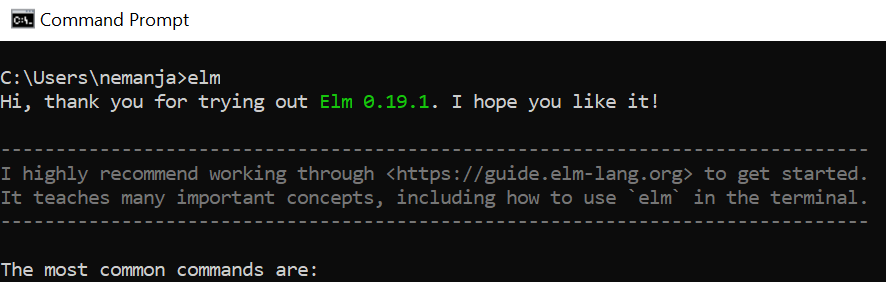
\includegraphics[width=0.95\textwidth]{elm-cmd.png}
  \caption{Provera uspešne instalacije \emph{Elm}-a}
  \label{fig:elm-cmd}
\end{figure}

\section{Osnovne odlike}
Pored \emph{No Runtime Exceptions}, jedna od glavnih odlika ovog jezika jeste
kompilator, koji je izuzetno ugodan za rad. Mnogi programeri smatraju da \emph{Elm}
kompilator proizvodi najbolje poruke o greškama. Za razliku od drugih, \emph{Elm}
kompilator objašnjava zašto je došlo do greške i daje predloge za njihovo rešavanje,
a takođe nema kaskadnih poruka. Kreator se vodio razmišljanjem da kompilator treba
da bude asistent, ne samo alat.

\emph{Elm} koristi svoju verziju \emph{virtuelnog DOM\footnote{DOM --- Obejektni model
dokumenta (eng. \emph{Document Object Model})\cite{dom}}-a}, koncepta koji se koristi u mnogim
razvojnim okvirima klijentskog programiranje. Ideja je da se u memoriji čuva "virtuelna" reprezentacija
korisničkog interfejsa na osnovu koje se ažurira "stvarni" \emph{DOM}. Još jedna bitna
karakteristika je nepromenljivost podataka, što znači da se jednom definisani
podaci ne mogu više menjati. Direktna posledica nepromenljivosti podataka je veoma
brzo iscrtavanje \emph{HTML}-a, jer se poređenja u virtuelnom \emph{DOM}-u mogu vršiti po referenci. 
Verzija \emph{Elm 0.17} imala je najbrže iscrtavanje u poređenju sa tadašnjim aktuelnim verzijama 
popularnih okvira\cite{elm-html}.

\emph{Elm} se može integrisati i u postojeće \emph{JavaScript} projekte za implementaciju pojedinačnih 
komponenti. Takođe, moguća je i komunikacija između ova dva programska jezika. 

\section{Elm kao platforma}
\emph{Elm} sa sobom donosi alat (tabela \ref{table:elmTools}) i okruženje \emph{Elm} (eng. \emph{Elm 
Runtime}), koji su neophodni za razvoj i izvršavanje aplikacija. \emph{Elm} k\^{o}d se nalazi u 
datotekama sa ekstenzijom \emph{.elm} i prilikom kompilacije kreira se jedna izlazna 
\emph{.js} datoteka. U izlaznoj datoteci se pored prevedenog koda iz ulaznih \emph{.elm} 
datoteka nalaze i funkcije iz okruženja \emph{Elm} potrebne za izvršavanje programa.

\begin{table}[h!]
\centering
\begin{tabular}{|l l|} 
 \hline 
 Alat & Kratak opis  \\ [0.5ex] 
 \hline
  \textbf{repl} & Pokretanje interaktivne sesije (eng. \emph{Read-Eval-Print-Loop}) \\ 
  \textbf{init} & Inicijalizacija projekta \\
  \textbf{reactor} & Pokretanje lokalnog servera \\
  \textbf{make} & Upotreba kompilatora \\
  \textbf{install}  & Preuzimanje paketa \\ 
  \textbf{diff} & Prikazivanje razlika između različitih verzija istog paketa \\
  \textbf{bump} & Određivanje broja naredne verzije paketa  \\
  \textbf{publish} & Objavljivanje paketa \\[1ex] 
 \hline
\end{tabular}
\caption{\emph{Elm} alatke komandne linije}
\label{table:elmTools}
\end{table}

 
Kao zaseban jezik \emph{Elm} ima i zaseban sistem za upravljanje paketima.
Pokretanjem komande \textbf{elm init} kreira se prazan direktorijum \emph{src} i 
datoteka \emph{elm.json}, u kojoj se pored informacije o tipu projekta (aplikacija ili 
paket), \emph{Elm} verzije i liste direktorijuma sa kodom, nalazi i spisak paketa koji se 
koriste u projektu. Dodavanje novog paketa se vrši pomoću komande \textbf{elm install} 
\emph{naziv-paketa}. Svi paketi su javno dostupni (\url{https://package.elm-lang.org/}),
nazivi paketa su oblika \emph{autor/ime-paketa}.

Kompilacija se vrši naredbom \textbf{elm make} \emph{<jedna-ili-više-elm-datoteka>},
ukoliko se ne navede izlazna datoteka pomoću argumenta \emph{-{}-output} generisaće 
se datoteka \emph{index.html} sa prevedenim \emph{JavaScript} kodom. Ostali argumenti kao i
više informacija o drugim alatkama mogu se videti pomoću naredbe \textbf{elm}
\emph{naziv-alata} \textbf{-{}-help}.

\section{Uticaj drugih progamskih jezika na Elm}
Kao i većina statički tipiziranih funkcionalnih programskih jezika, \emph{Elm} se zasniva na
programskom jeziku \emph{ML}, a budući da su u programskom jeziku \emph{Haskell} napisani \emph{Elm} kompilator
i ostale alatke, \emph{Haskell} je ostavio veliki uticaj i na sam jezik. Autor \emph{Elm}-a smatra:
\begin{displayquote}
"Rekao bih da \emph{Elm} pripada porodici \emph{ML} jezika, sa sintaksom poput \emph{Haskell}-a. Ako poredimo semantiku,
\emph{Elm} je dosta sličniji \emph{OCaml}-u i \emph{SML}-u." \cite{eczaplicki:2015}
\end{displayquote}

\textbf{ML} (eng. \emph{Meta Language})\cite{ml} je statički tipiziran programski jezik opšte 
namene koji je nastao 1973. godine na Univerzitetu u Edinburgu. Vođa grupe koja je radila
na dizajniranju programskog jezika ML bio je Robin Milner, dobitnik Tjuringove nagrade.
Nastao je pod uticajem programskog jezika LISP, a razvijan je za implementiranje automatskog
dokazivača teorema. Osnovna karakteristika jeste uvođenje automatskog zaključivanja tipova, a
odlikuje ga i poklapanje obrazaca, Karijeve funkcije i posedovanje sakupljača otpadaka. ML
nije čist funkcionalan jezik i nema ugrađenu podršku za lenjo izračunavanje. U porodicu ML 
jezika, između ostalih, spadaju i \textbf{Standard ML}, \textbf{OCaml} i \textbf{F{\#}}.


\textbf{Haskell}\cite{haskell} je čist funkcionalni programski, naziv je dobio po matematičaru i 
logičaru Haskelu Bruks Kariju (eng. \emph{Haskell Brooks Curry}). \emph{Haskell} je strogo 
tipiziran, poseduje automatsko zaključivanje tipova i lenjo izračunavanje. Jezik je 
opšte namene, pruža podršku za paralelno i distribuirano programiranje. \emph{Haskell} 
omogućava manje grešaka i veću pouzdanost kroz kraći i čistiji k\^{o}d, koji je lakši za
održavanje. 

\section{Elm kao jezik}
U ovom poglavlju predstavljene su osnovne programskog jezika Elm --- osnovni tipovi i strukture podataka,
operatori, način definisanja i grupisanja funkcija, navođenje komentara, kontrola toka i obrada grešaka.

\subsection{Komentari}
Komentari u \emph{Elm}-u se mogu navoditi na dva načina: \begin{itemize}
  \item Korišćenjem \texttt{-{}-} za linijske komentare
  \item Navođenjem teksta između znakova \texttt{\{-} i \texttt{-\}} za komentare u više redova.    
\end{itemize}

\subsection{Osnovni tipovi podataka}
\begin{listing}[h]
\begin{minted}{haskell}
> 'Z'
'Z' : Char
> "Zdravo!"
"Zdravo!" : String
> True
True : Bool
>42
42 : number
> 42 / 10 
4.2 : Float
> 42 // 10 --celobrojno deljenje
4 : Int
\end{minted}
\caption{Osnovni tipovi podataka prikazani u interpretatoru}
\label{listing:tipovi}
\end{listing}
Osnovni tipovi podataka programskog jezika \emph{Elm} su \textbf{Char}, \textbf{String}, \textbf{Bool},
\textbf{Int} i \textbf{Float}. U primeru koda \ref{listing:tipovi} prikazani su osnovni
tipovi korišćenjem interpretatora (\texttt{\textbf{elm repl}}). Budući da i \emph{Elm} poseduje zaključivanje tipova, nakon
izračunate vrednosti unetog izraza ispisuje se tip. U konkretnom primeru broj 42 se
može posmatrati i kao tip \textbf{Int} i kao tip \textbf{Float}, pa interpretator vraća
\texttt{number} kao tip, iako \texttt{number} nije konkretan tip podataka već poseban oblik tipske promenljive.
Tipske promenljive objašnjene su dalje u posebnom poglavlju.


Tip \textbf{Char} služi za predstavljanje junikod (eng. \emph{unicode}) karaktera.
Karakteri se navode između dva apostorfa (\texttt{'a', '0', '\textbackslash t'}...), a
moguće je koristiti i junikod zapis \texttt{'\textbackslash u\{0000\}}' -
\texttt{'\textbackslash u\{10FFFF\}'}.

Za razliku od programskog jezika \emph{Haskell}, gde je niska (\textbf{String}) zapravo lista karaktera, u \emph{Elm}-u je
poseban tip i predstavlja sekvencu junikod karaktera. Sekvenca se navodi između
jednostrukih ili trostrukih navodnika (primer koda \ref{listing:string}).

\begin{listing}[ht]
\begin{minted}{haskell}
> "\t Niska u jednom redu: escape navodnici \"Zdravo!\""
"\t Niska u jednom redu: escape navodnici \"Zdravo!\"" : String
>
> """Niska u više redova
 sa "navodnicima"! """
"Niska u više redova\n  sa \"navodnicima\"! " : String
\end{minted}
\caption{Primeri niski}
\label{listing:string}
\end{listing}

Tip \textbf{Bool} predstavlja logički tip i može imati vrednost \texttt{True} ili
\texttt{False}. 

Tip \textbf{Int} se koristi za prikazivanje celih brojeva. U trenutnoj verziji (\emph{0.19.1}) opseg vrednosti je
od \(-2^{53}\) do \(2^{53} - 1\). Vrednosti se mogu navoditi i u heksadecimalnom obliku (\texttt{0x2A, -0x2b}).

Tip \textbf{Float} služi za predstavljanje brojeva u pokretnom zarezu po strandardu
\emph{IEEE 754}. Vrednosti se mogu navoditi i pomoću eksponencijalnog zapisa, a decimalna 
tačka se mora nalaziti između dve cifre. Takođe, u skup vrednosti spadaju \texttt{NaN} i
\texttt{Infinity} (primer koda \ref{listing:brojevi}).

\begin{listing}[ht]
\begin{minted}{haskell}
> 1e3
1000 : Float
> 0/0 
NaN : Float
> 1/0 
Infinity : Float
\end{minted}
\caption{Prikaz brojeva u pokretnom zarezu}
\label{listing:brojevi}
\end{listing}


\subsection{Osnovni operatori}
Kod aritmetičkih operacija, operatori \texttt{+, -, *} se mogu koristiti sa realnim i 
celim brojevima, dok imamo posebne operatore za deljenje (\texttt{{/}} i \texttt{{//}} koji
su i ranije prikazani u primeru koda \ref{listing:tipovi}). \emph{Elm} ne podržava implicitne konverzije
tipova, pa prilikom sabiranja celog broja sa realnim, bez eksplicitne konverzije, kompilator
prijavljuje grešku (primer koda \ref{listing:konverzija}). Postoji još i eksponencijalni operator \^{},
a za celobrojno deljenje sa ostatkom koriste se funkcije \texttt{modBy} i \texttt{remainderBy}.
\begin{listing}[h]
\begin{minted}{haskell}
> toFloat (9 // 3) + 3.2
6.2 : Float
> 9 // 3 + round 3.2
6 : Int
> 9 // 3 + 3.2 -- TYPE MISMATCH error
\end{minted}
\caption{Upotreba eksplicitne konverzije tipova}
\label{listing:konverzija}
\end{listing}

Od relacijskih operatora \texttt{==, /=, <, >, >= i <=}, jedino operator različitosti (\texttt{/=}) ima drugačiju
sintaksu od uobičajene. Prioriteti između relacijskih operatora nisu definisani i prilikom njihovog kombinovanja
izrazi se moraju odvojiti zagradama.
\emph{Elm} pruža logičke operatore \emph{i} \texttt{\&\&} i \emph{ili} \texttt{||} kao i funkcije za negaciju 
\texttt{not} i ekskluzivno ili \texttt{xor}. Operator \texttt{\&\&} ima viši prioritet 
od operatora \texttt{||}, oba su levo asocijativna i lenjo izračunljiva. Pored navednih, \emph{Elm} podržava i operator \texttt{++} koji se koristi za
konkatenaciju niski i listi. Primer koda \ref{listing:operatori} prikazuje upotrebe 
navedenih operatora.

\begin{listing}[h]
\begin{minted}{haskell}
> 2 > 3 == 3 > 4 
-- INFIX PROBLEM - You cannot mix (>) and (==) without parentheses.
> (2 > 3) == (3 > 4)
True : Bool
> not (1 + 1 /= 2) && 2 + 2 <= 5 || 1^0 == 0^1 
True : Bool
> 2^6 - 0x100 / 4  * (1 + 2)
-128 : Float
> "Spojena " ++ "niska!" == "Spojena niska!"
True : Bool
\end{minted}
\caption{Primeri upotrebe osnovnih operatora}
\label{listing:operatori}
\end{listing}

\subsection{Funkcije}  
Sintaksa za definisanje funkcija je veoma jednostavna i prikazana je u primeru koda 
\ref{listing:funkcije}.
\begin{listing}[h]
\begin{minted}{haskell}
{-
  nazivFunkcije param1 param2 ... =
    izraz  
-}
deljivSa x y =
  modBy x y == 0

dobarDan x = "Dobar dan, " ++ x ++ "!"  
\end{minted}
\caption{Primeri definisanja funkcija}
\label{listing:funkcije}
\end{listing}

Ime funkcije obavezno počinje malim slovom, nakon čega sledi niz slova (velikih i malih),
simbola \texttt{\textbf{\textunderscore}} i brojeva. Po konvenciji, sva slova se navode u
neprekidnoj sekvenci, stoga je preporučena kamilja notacija (\texttt{camelCase}).
Parametri se odvajaju razmakom, dok se zagrade ne navode ni prilikom definisanja, ni
pozivanja funkcije. Ipak, primena funkcije je levo asocijativna, pa je česta upotreba
zagrada za ograđivanje izraza. Telo funkcije predstavlja jedan jedini izraz koji se izvršava
prilikom pozivanja, a izračunata vrednost predstavlja povratnu vrednost funkcije.
Izraz se, po konvenciji, piše u novom redu, ali je moguće i u istom.

Funkcije u \emph{Elm}-u mogu prihvatati funkcije kao parametre i vraćati funkcije kao 
povratne vrednosti, što ih čini funkcijama višeg reda. Nije moguće navoditi
podrazumevane vrednosti parametara, kao ni preopterećivanje funkcija.


\subsubsection{Konstante}
U programskom jeziku \emph{Elm} ne postoje promenljive, jednom definisani podaci se ne mogu promeniti, ali je 
moguće definisati konstante. Često se u literaturi definisanje konstanti naziva 
\emph{imenovanjem vrednosti izraza} i ne dovodi se u vezu sa funkcijama, ali se konstante 
mogu posmatrati kao \emph{konstantne funkcije}, koje se izvrše tokom kompilacije. Definišu se
kao i funkcije, ali bez parametara (primer koda \ref{listing:lambda}).

\subsubsection{Anonimne funkcije}
Anonimne funkcije se definišu slično kao i regularne, umesto imena navodi se simbol 
\texttt{\textbf{\textbackslash}} koji predstavlja grčko slovo lambda - \(\lambda\),
dok se simboli \texttt{\textbf{->}} koristi umesto znaka pridruživanja (primer koda \ref{listing:lambda}).
\begin{listing}[h]
\begin{minted}{haskell}
> broj3 = 3
3 : number
> (\x y -> x + y) broj3 4
7 : number
\end{minted}
\caption{Primer anonimne funkcije}
\label{listing:lambda}
\end{listing}

\subsubsection{Tip funkcije}
Prilikom definisanja funkcije u interpretatoru ili
poziva funkcije bez parametara, kao vrednost izraza vraća se \texttt{\textbf{<function>}} 
i tip funkcije. U primeru koda \ref{listing:tipoviFunkcije} prikazano je nekoliko 
tipova funkcija u interpretatoru.
\begin{listing}[h]
\begin{minted}{haskell}
> not
<function> : Bool -> Bool
> deljivSa
<function> : Int -> Int -> Bool
> \x y z -> x + y + z
<function> : number -> number -> number -> number
> deljivSa 3 --parcijalna primena
<function> : Int -> Bool
\end{minted}
\caption{Tipovi funkcija}
\label{listing:tipoviFunkcije}
\end{listing} 
  
U primeru funkcije \texttt{\textbf{not}} vidimo da je njen tip \emph{Bool -> Bool},
što je na prvi pogled jasno i znači da se radi o funkciji jednog argumenta koja
prihvata vrednost tipa \emph{Bool} i vraća vrednost tipa \emph{Bool}. 
U slučaju funkcije \texttt{\textbf{deljivSa}} i anonimne funkcije koja sabira tri broja,
tip funkcije se može posmatrati tako da poslednji tip u nizu koji je razdvojen strelicama
(\texttt{\textbf{->}}) predstavlja povratni tip funkcije, dok tipovi pre njega 
predstavljaju tipove argumenata funkcije. Tipovi argumenata su takođe odvojeni strelicama
jer su sve funkcije u programskom jeziku \emph{Elm} zapravo Karijeve (\emph{Curried}) funkcije (slika \ref{fig:currying}),
što znači da su funkcije jednog argumenta koje kao povratnu vrednost imaju funkciju.
\begin{figure}[!h]
  \centering
  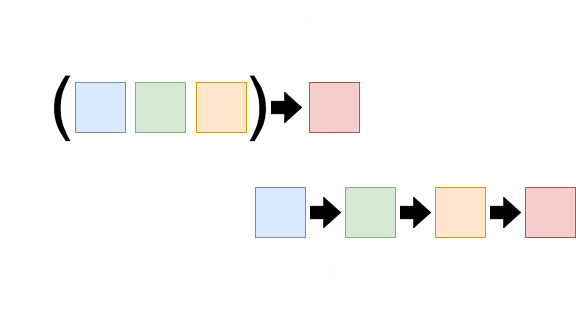
\includegraphics[width=0.5\textwidth]{currying.png}
  \caption{Regularne i Karijeve funkcije}
  \label{fig:currying}
\end{figure}
Strelica (\texttt{\textbf{->}}) je desno asocijativna, a zagrade se izostavljaju zbog
jednostavnosti. Na primer, funkcija \texttt{deljivSa} ima tip \emph{Int -> (Int -> Bool)},
što znači da prihvata vrednost tipa \emph{Int} i vraća funkciju tipa \emph{Int -> Bool}.
Karijeve funkcije nam omogućavaju veću fleksibilnost i parcijalnu primenu funkcija, 
odnosno vezivanje argumenata za konkretne vrednosti (primer koda \ref{listing:tipoviFunkcije}).

\subsubsection{Anotacija tipa funkcije}
Kao što je prethodno prikazano, \emph{Elm} sam zaključuje tip funkcije, ali dozvoljava i korisniku
da sam navede tip u liniji iznad definicije (primer koda \ref{listing:anotacija}).
\begin{listing}[!h]
\begin{minted}{haskell}
> deljivSa: Int -> Int -> Bool
| deljivSa x y =
|   modBy x y == 0
|
<function> : Int -> Int -> Bool
\end{minted}
\caption{Anotacija tipa funkcije}
\label{listing:anotacija}
\end{listing}

Korišćenje anotacije tipova nije obavezno, ali je vrlo preporučljivo iz više razloga.
Prilikom kompilacije proverava se poklapanje anotacije sa stvarnim tipom funkcije, što
dovodi do lakšeg uočavanja i otklanjanja grešaka. Pored toga, anotacije predsavljaju veoma
dobar vid dokumentacije, a činjenica da kompilator uvek poredi navedeni i stvarni tip nam
garantuje da je dokumentacija uvek važeća.

\subsubsection{Funkcijski operatori}
Operatore nad funkcijama možemo podeliti prema tipu, na operatore prosleđivanja i operatore
kompozicije funkcija, i prema smeru u kom se primenjuju, unapred ili unazad.

Operatori prosleđivanja ili \textbf{pipe} operatori su zapravo operatori primene funkcije
i omogućavaju pisanje čitljivijeg koda sa manje zagrada.
\begin{itemize}
  \item \texttt{\textbf{<|}} - pipe operator unazad radi isto što i primena funkcije, 
  s tim što nas oslobađa pisanja zagrada. Preciznije, \texttt{\textbf{f <| x}} je drugi zapis
  za \texttt{\textbf{f (x)}}
  \item \texttt{\textbf{|>}} - pipe operator inspirisan je Unix pipe-om, odatle i
  naziv, i služi za prosleđivanje argumenta funkciji. Preciznije, \texttt{\textbf{x |> f}}
  je drugi zapis za \texttt{\textbf{f (x)}}
\end{itemize}

Operator kompozicije unazad \texttt{\textbf{<\smallskip<}} predstavlja operator matematičke 
kompozicije funkcija \(\circ\). Tako da se definicija kompozicije dve funkcije, \((g \circ f)(x) = g(f(x))\),
u programskom jeziku \emph{Elm} može posmatrati kao: \texttt{\textbf{(g <\smallskip< f) x == (\textbackslash x\textunderscore ->
g ( f x\textunderscore)) x}}. Operator kompozicije \texttt{\textbf{>\smallskip>}} je
simetričan operatoru \texttt{\textbf{<\smallskip<}}, stoga važi: \texttt{\textbf{(f <\smallskip< g) x == (g >\smallskip> f) x}}.


\subsubsection{Moduli}
Moduli se koriste za grupisanje funkcija u logičke jedinice i kreiranje imenskih 
prostora (eng. \emph{namespace}). Osnovni tipovi, kao i funkcije i operatori nad njima 
definisani su u modulu \texttt{\textbf{Basics}}, koji je podrazumevano uvezen i nalazi se 
unutar paketa \texttt{\textbf{elm/core}}. Svaki modul predstavlja jednu \emph{.elm} datoteku,
koja se mora zvati isto kao i modul, dok ime modula mora počinjati velikim slovom.
Za definisanje modula koristi se ključna reč \texttt{\textbf{module}} nakon koje sledi
ime modula, ključna reč \texttt{\textbf{exposing}} i lista funkcija kojima se može 
pristupiti van modula.
\begin{listing}[h]
\begin{minted}{haskell}
module Krug exposing (povrsina, obim) 
-- module Krug exposing (..) - otrkivanje svega iz modula 
pi = 3.14

povrsina r =
    naKvadrat r * pi

obim r =
    2 * r * pi

naKvadrat x =
    x * x
\end{minted}
\caption{Primer modula}
\label{listing:modul}
\end{listing}

Da bi se modul iz primera koda \ref{listing:modul} koristio u interpretatoru (\texttt{\textbf{elm repl}}),
prvo je potrebno inicijalizovati \emph{Elm} projekat (\texttt{\textbf{elm init}}) i u direktorijumu \texttt{src} napraviti 
datoteku \emph{Krug.elm} sa prikazanim sadržajem. Zatim, u interpretatoru naredbom 
\texttt{\textbf{import}} treba uvesti modul. Načini korišćenja funkcija iz modula
\emph{Krug} prikazani su u primeru koda \ref{listing:import}.
\begin{listing}[h]
\begin{minted}{haskell}
import Krug                           -- Krug.obim Krug.povrsina
import Krug as K                      -- K.obim K.povrsina

import Krug exposing (obim)           -- obim, Krug.povrsina
import Krug exposing (..)             -- obim, povrsina
import Krug as K exposing (povrsina)  -- K.obim, povrsina
\end{minted}
\caption{Primer korišćenja modula}
\label{listing:import}
\end{listing}

\subsection{Osnovne strukture podataka}
Osnovne strukture podatka programskog jezika \emph{Elm} čine liste, torke i slogovi. 
\subsubsection{Liste}
Lista predstavlja kolekciju u obliku jednostruko povezane liste. Elementi se navode
unutar uglastih zagrada---\textbf{\texttt{[\smallskip ]}} i moraju biti istog tipa. Funkcije za rad
sa listama nalaze se unutar modula \texttt{List}, među kojim su i tri veoma važne funkcije višeg reda
u funkcionalnoj paradigmi --- \textbf{\texttt{map, filter}} i \textbf{\texttt{fold}} (
\textbf{\texttt{reduce}} ili \textbf{\texttt{accumulate}} u drugim programskim jezicima). 

Funkcija \textbf{\texttt{map}} prihvata funkciju i listu i primenjuje datu funkciju na svaki elemenat
liste čime se kreira nova lista. Funkcija \textbf{\texttt{filter}} prihvata predikat (funkciju koja
vraća logičku vrednost) i listu, a vraća novu listu koja sadži samo elemente koji zadovoljavaju dati predikat.
Funkcije \textbf{\texttt{fold}} koriste se za "savijanje" liste u jednu vrednost koja se često naziva akumulator.
U zavisnosit od smera "savijanja" --- da li se ide sa početka ili kraja liste koriste se leva (\textbf{\texttt{foldl}}),
odnosno desna (\textbf{\texttt{foldr}}) funkcija. Funkcije (\textbf{\texttt{fold}}) prihvataju binarnu funkciju,
početnu vrednost akumulatora i listu i prilikom prolaska kroz elemnte liste primenjuje se data funkcija
nad trenutnim elementom i akumulatorom čime se kreira nova vrednost akumulatora. Tipovi navedenih funkcija prikazani su u
primeru koda \ref{listing:listFnTypes}, a njihova upotreba u primeru koda \ref{listing:liste}.
\begin{listing}[h]
\begin{minted}{haskell}
> List.map
<function> : (a -> b) -> List a -> List b
> List.filter
<function> : (a -> Bool) -> List a -> List a
> List.foldl
<function> : (a -> b -> b) -> b -> List a -> b
\end{minted}
\caption{Tipovi funkcija \texttt{map, filter} i \texttt{foldl}}
\label{listing:listFnTypes}
\end{listing}

Pored operatora za nadovezivanje \textbf{\texttt{++}}, postoji i operator \textbf{\texttt{::}} koji
dodaje element na početak liste, iz istorijskih razloga ovaj operator naziva se kons
(eng. \emph{cons}). 
\begin{listing}[h]
\begin{minted}{haskell}
> "aaa" :: ["bbb","ccc"]
["aaa","bbb","ccc"] : List String
> List.map (List.member 2) [[1,2,3],[2,2],[42]]
[True,True,False] : List Bool
> [1,2]++[3,4,5] |> List.filter (\x -> modBy 2 x == 0) |> List.length
2 : Int
> List.foldl (\acc x -> acc + x) 0 <| List.range 1 5 
15 : Int
\end{minted}
\caption{Primeri lista različitih tipova i funkcija za rad sa njima}
\label{listing:liste}
\end{listing}
\subsubsection{Torke}
Za razliku od listi koje mogu imati promenljivi broj elemenata istog tipa, torke
predstavljaju kolekcije fiksne dužine čiji elementi ne moraju biti istog tipa.
Mogu sadržati samo dva ili tri elementa, navode se unutar običnih zagrada---
\textbf{\texttt{()}}. U torke se ne mogu ubacivati elementi niti se iz torke mogu
uklanjati elementi. Funkcije nad torkama koje imaju dva elementa nalaze se u modulu
\texttt{Tuple}, dok se za rad sa tokrama od tri elementa koristi poklapanje obrazaca
o kojem će biti više reči kasnije.
\begin{listing}[h]
\begin{minted}{haskell}
> (1,"2",'3')
(1,"2",'3') : ( number, String, Char )
> (1,2) == Tuple.pair 1 2
True : Bool
> Tuple.second ("nebitan", "drugi")
"drugi" : String
> Tuple.mapFirst String.length ("mapiran", 1)
(7,1) : ( Int, number )
\end{minted}
\caption{Primeri torki i upotreba funkcija iz modula \texttt{Tuple}}
\label{listing:torke}
\end{listing}
\subsubsection{Slogovi} 
Slog (eng. \emph{Record}) predstavlja strukturu podataka koja može sadržati više vrednosti različitih tipova, 
pri čemu je svakoj vrednosti dodeljen naziv. Liče na \emph{JavaScript} objekte, čak je i 
sintaksa veoma slična, umesto dvotačke slog koristi znak jednakosti za dodelu naziva.
Prilikom definisanja sloga, \emph{Elm} kreira funkcije za pristup njegovim svojstvima. Nije 
moguće dodavanje, ni uklanjanje svojstava, ali je dozvoljena promena njihovih vrednosti.
Zbog imutabilnosti, ne vrši se promena nad postojećim slogom već se pravi novi.
\begin{listing}[h]
\begin{minted}{haskell}
> pera = {ime = "Pera", prezime = "Perić", godine = 23}
{ godine = 23, ime = "Pera", prezime = "Perić" } 
  : { godine : number, ime : String, prezime : String }
> {pera | prezime = "Petrović", godine = 24}
{ godine = 24, ime = "Pera", prezime = "Petrović" }
  : { godine : number, ime : String, prezime : String }
> pera.ime
"Pera" : String
> .godine pera
23 : number
> .prezime
<function> : { b | prezime : a } -> a
\end{minted}
\caption{Primeri pristupa i promene svojstava sloga}
\label{listing:rekord}
\end{listing}

Pored navedenih struktura podataka, \emph{Elm} pruža podršku za rad sa nizovima (\texttt{Array}),
skupovima (\texttt{Set}) i rečnicima (\texttt{Dict}).

\subsection{Tipske promenljive} 
U primeru koda \ref{listing:rekord} vidimo da funkcija za pristup prezimenu ima tip:\\ 
\texttt{\textbf{\{ b | prezime : a \} -> a}}. Ovo znači da funkcija kao argument
prima slog, koji može biti bilo kog tipa, ali mora imati svojstvo\texttt{\textbf{
prezime}}, koje takođe može biti bilo kog tipa, i čiji tip je ujedno povratni tip 
funkcije. Promenljive \texttt{\textbf{a}} i \texttt{\textbf{b}} nazivaju se 
\emph{tipske promenljive}, a prisustvo dve tipske promenljive nam govori da one mogu, 
ali ne moraju, predstavljati različite tipove. U konkretnom primeru \texttt{\textbf{a}}
i \texttt{\textbf{b}} su uvek različitog tipa, dok u slučaju funkcije \texttt{Tuple.pair
: a -> b -> ( a, b )} mogu biti istog tipa. Prilikom anotacije tipova mogu se koristi i
duža imena tipskih promenljivih, a pravlia imenovanja su ista kao i za funkcije.

Tipske promenljive u programskom jeziku \emph{Elm} ukazuju na prisustvo \textbf{parametarskog polimorfizma},
jedine vrste polimorfizma u ovom jeziku.

\subsubsection{Uslovne tipske promenljive}
Za razliku od programskog jezika \emph{Haskell}, \emph{Elm} nema toliko složen sistem tipova i umesto tipskih 
klasa (eng. \emph{typeclasses})\cite{typeclasses} poseduje jednostavniji koncept
---\emph{uslovne tipske promenljive}. 

Uslovne tipske promenljive omogućavaju da se na određni način ograniči skup tipova
koji se može koristiti u izrazima. Najčešći primer je \texttt{number}, koji dozvoljava 
isključivo \texttt{Int} ili \texttt{Float} tipve. 

U trenutnoj verziji (\emph{0.19.1}) postoje četiri uslovne tipske promenljive:
\begin{enumerate}
  \item \texttt{number} --- dozvoljava tipove \texttt{Int} i \texttt{Float}
  \item \texttt{appendable} --- dozvoljava tipove \texttt{String} i \texttt{List a}
  \item \texttt{comparable} --- dozvoljava tipove \texttt{Int}, \texttt{Float}, \texttt{Char},
  \texttt{String}, liste i torke koje sadrže \texttt{comparable} vrednosti
  \item \texttt{compappend} --- dozvoljava tipove \texttt{String} i \texttt{List comparable}
\end{enumerate}
\subsubsection{Operatori i tipske promenljive}

\begin{listing}[h]
\begin{minted}{haskell}
> (+) 1 2
3 : number
> (*)
<function> : number -> number -> number
> (++)
<function> : appendable -> appendable -> appendable
> (==)
<function> : a -> a -> Bool
> (>=)
<function> : comparable -> comparable -> Bool
\end{minted}
\caption{Upotreba operatora u prefiksnoj notaciji}
\label{listing:tipskePromenljive}
\end{listing}
Operatori predstavljaju funkcije koje se mogu pozivati u infiksnoj notaciji. Takođe, 
mogu se pozivati i u prefiksnoj ukoliko ih navedemo unutar zagrada: \texttt{\textbf{(+),
(++), (>=)}}... , dok pozivanjem bez argumenata možemo videti i kog su tipa (primer koda \ref{listing:tipskePromenljive}).

U ranijim verzijama jezika bilo je moguće definisati korisničke operatore, ali je ta
opcija izbačena u verziji \emph{0.19.0}, a od verzije \emph{0.18.0} nije moguće pozivanje 
binarnih funkcija u infiksnoj notaciji.

\subsection{Alijasi tipova}
Prilikom definisanja funkcija koje rade nad istim strukturama podataka višestruko navodimo
iste anotacije tipova, pritom anotacije podataka mogu biti predugačke, samim tim i
teško čitljive. Alijasi tipova nam omogućavaju ponovnu upotrebu anotacija i bolju čitljivost.
Definišu se pomoću ključnih reči \texttt{\textbf{type alias}}, nakon kojih sledi ime koje
mora počinjati velikim slovom. 
\begin{listing}[h]
\begin{minted}{haskell}
>type alias MatricaInt3 = List (List (List Int))
>
>type alias Osoba = {ime : String, prezime : String, godine : Int }
> Osoba
<function> : String -> String -> Int -> Osoba
> Osoba "Pera" "Perić" 23
{ godine = 23, ime = "Pera", prezime = "Perić" } : Osoba
\end{minted}
\caption{Primeri definisanja alijasa tipova}
\label{listing:alias}
\end{listing}

Prilikom kreiranja alijasa za slog kreira se i konstruktor za slog, što se može videti
u primeru koda \ref{listing:alias}. Redosled argumenata funkcije za konstrukciju identičan je
redosledu u alijasu.
\subsection{Korisnički definisani tipovi}
Pored korišćenja alijasa za postojeće tipove podataka, \emph{Elm} pruža mogućnost kreiranja novih 
tipova. Korisnički definisani tipovi se često nazivaju algebarskim tipovima (eng. \emph{algebraic datatype}),
kao i \emph{unijskim} tipovi, jer mogu predstavljati uniju više varijanti definisanog tipa. Definišu se ključnom reči 
\textbf{\texttt{type}}, a varijante se odvajaju simbolom \texttt{\textbf{|}}.

Slično kao kod alijasa tipova za slogove i ovde se kreiraju konstruktori za definisani tip.
Bitna razlika u odnosu na alijase tipova je ta što algebarski tipovi mogu biti rekurzivni, tj.
tip koji se definiše se može navoditi unutar svoje definicije. U primeru koda \ref{listing:algebraic}
se mogu videti primeri definisanja algebarskih tipova i tipovi njihovih konstruktora. Takođe je prikazana
i definicija binarnog stabla kao primer rekurzivne strukutre.
\begin{listing}[h]
\begin{minted}{haskell}
> type VectorF4 = Vector4F Float Float Float Float
> Vector4F
<function> : Float -> Float -> Float -> Float -> VectorF4
>
>type StatusPrijave 
  = NaCekanju 
  | Greska String 
  | Uspesno {id : Int, token : String}
> NaCekanju
NaCekanju : StatusPrijave
> Greska
<function> : String -> StatusPrijave
> Uspesno
<function> : { id : Int, token : String } -> StatusPrijave
> type BinarnoStablo a 
  = PraznoStablo 
  | CvorStabla a (BinarnoStablo a) (BinarnoStablo a)
\end{minted}
\caption{ Primeri korisnički definisanih tipova}
\label{listing:algebraic}
\end{listing}

\subsection{Kontrola toka}
\emph{Elm} ne izvršava naredbe, već evaluira izraze, tako da umesto naredbi grananja
imamo izraze \texttt{\textbf{if}} i \texttt{\textbf{case}}, a funkcije višeg reda ili rekurziju umesto petlji.
\subsubsection{Izraz \texttt{\textbf{if}}}
Izraz \texttt{\textbf{if}} se može posmatrati kao ternarni operator u programskim jezicima \emph{JavaScript}, \emph{C++} i 
mnogim drugim.
\begin{listing}[h]
\begin{minted}{haskell}
{-    uslov   ?  izraz1   :  izraz2   - ternarni operator
   if uslov then izraz1 else izraz2   - if izraz
-}
if x >= 0 then "pozitivan" else "negativan"
if x == 1 then x * 2 else if x == 2 then x / 2 else x
\end{minted}
\caption{Sintaksa izraz \texttt{\textbf{if}} i primer upotrebe}
\label{listing:if}
\end{listing}

Ključna reč \texttt{\textbf{else}} je sastavni deo izraza \texttt{\textbf{if}} tako
da \texttt{\textbf{else}} "grana" uvek postoji. Mogu se navoditi i ugnježdeni
izrazi \texttt{\textbf{if}}, pa \texttt{\textbf{else if}} grana predstavlja korišćenje
izraza \texttt{\textbf{if}} nakon ključne reči \texttt{\textbf{else}}.

\subsubsection{Izraz \texttt{\textbf{case}}}
Za raliku od izraza \texttt{\textbf{if}}, izraz \texttt{\textbf{case}} omogućava grananje na
osnovu šireg raspona vrednosti, umesto samo sa \emph{tačno} ili \emph{netačno}. Takođe, pruža mogućnost navođenja više grana.
Primer upotrebe izaraza \texttt{\textbf{case}} prikazan je u primeru koda \ref{listing:case}. Vrednost navedena nakon ključne reči
\texttt{\textbf{case}} se redom upoređuje sa navedenim opcijama i prvim poklpanjem se određuje vrednost izraza.
\begin{listing}[h]
\begin{minted}{haskell}
case mesto of
  1 -> "zlato"
  2 -> "srebro"
  3 -> "bronza"
  _ -> "zahvalnica"
\end{minted}
\caption{Primer upotrebe izraza \texttt{\textbf{case}}}
\label{listing:case}
\end{listing}

Prilikom korišćenja izraza \texttt{\textbf{case}} moraju se pokriti sve
mogućnosti, ukoliko to nije slučaj kompilator prijavljuje grešku. Za podrazumevani slučaj
može se korisiti simbol \texttt{\textbf{\textunderscore}}. Izraz \texttt{\textbf{case}}
zauzima značajno mesto u programskom jeziku \emph{Elm}, jer se koristi u \textbf{poklapanju obrazaca}.

\subsubsection{Izraz \texttt{\textbf{let}}}
Budući da ne postoje blokovi naredbi, izrazi \texttt{\textbf{let}} nam omogućavaju da 
ograničimo oblast važenja --- dosega (eng. \emph{scope}) funkcija i konstanti u okviru
jedne funkcije. Doprinose boljoj čitljivosti koda, a moguće je koristiti anotacije tipova
unutar njih.
\begin{listing}[h]
\begin{minted}{haskell}
let
  nula: Int
  nula = 0
  
  pozitivan: Int -> Bool
  pozitivan =
    \x -> x > nula
in pozitivan 10
\end{minted}
\caption{Primer upotrebe izraza \texttt{\textbf{let}}}
\end{listing}
\subsubsection{Rekurzija}
Rekurzivno definisana funkcija poziva samu sebe, čime se postiže ponavljanje izvršavanja
koje se u imperativnom programiranju ostvaruje korišćenjem petlji (ili takođe rekurzijom).
U mnogim slučajevima, umesto rekurzije mogu se koristiti funkcije višeg reda i treba ih
upotrebiti kad god je to moguće.
\begin{listing}[h]
\begin{minted}{haskell}
factorial n = 
  if n <= 1 then 1 
  else  n * factorial (n - 1)

factorialFold n = 
  List.foldl (*) 1 (List.range 1 n) 
\end{minted}
\caption{Upotreba rekurzije i funkcije \texttt{foldl} za iteraciju kroz listu}
\end{listing}

\subsection{Poklapanje obrazaca}
Poklapanje obrazaca (eng. \emph{pattern matching}) može se posmatrati kao pokušavanje usklađivanja (poklapanja) ulaznog
podatka sa unapred definisanim obrascem. Ukoliko dođe do usklađivanja, poklopljenim
vrednostima se može prisupiti putem identifikatora definisanim u obrascu. Pored spomenutih
\texttt{\textbf{case}} izraza, poklapanje obrazaca može se korisiti u vidu 
razlaganja slogova ili torki prilikom definisanja funkcija ili korišćenja \texttt{\textbf{let}} izraza.
\begin{listing}[h]
\begin{minted}{haskell}
-- liste 
case lista of
  [] -> "prazna lista"
  [_] -> "jedan element"
  [a,b] -> "dva elementa: " ++ a ++ " i " ++ b
  a :: _ -> "više od dva elemenata, prvi je: " ++ a

-- unijski tipovi
case prijava of
  NaCekanju -> "Molimo za strpljejne"
  Greska poruka -> "Došlo je do grške: " ++ poruka
  Uspesno {id} -> "Uspešna prijava, id: " ++ String.fromInt id

-- torke
case tacka3D of
  (0, 0, 0) -> "centar"
  (0, _, _) -> "na x-osi"
  _ -> "van x-ose"

-- razlaganje
let
  (x,_,_) = tacka3D
in "x koordinata je " ++ String.fromFloat x

--nije moguće poklapanje ugnježdenih slogova
prikaziPodatke ({ime, adresa} as osoba) =
  ime ++ " " ++ osoba.prezime ++ " " ++ adresa.ulica
\end{minted}
\caption{Primeri poklapanja obrazaca}
\label{listing:poklapanjeObrazaca}
\end{listing}

Unutar case izraza sekvencijalno se vrši poklapanje obrazaca. Kada dođe do poklapanja
izračunava se izraz dodeljen datom obrascu, ne nastavlja se sa poklapanjem. Kompilator
prepoznaje ukoliko može doći do nepoklapanja nijednog obrasca i prijavljuje grešku.
Takođe, greška se prijavljuje i ukoliko se navede redudantan obrazac, tj. obrazac čiji se
skup vrednosti preklapa sa skupom vrednosti prethodno definisanog obrasca.
Simbol \texttt{\textbf{\textunderscore}} služi za poklapanje vrednosti koje se ne koriste,
a ključna reč \texttt{\textbf{as}} se može koristiti ukoliko je potrebno pristupiti celom
ulaznom podatku. U primeru koda \ref{listing:poklapanjeObrazaca} mogu se videti primeri
poklapanja obrazaca.

\subsection{Obrada grešaka pomoću \texttt{\textbf{Maybe}} i \texttt{\textbf{Result}}}
Unutar programskog jezika \emph{Elm} ne postoje \texttt{\textbf{try catch}} blokovi, kao ni \texttt{\textbf{undefined, null, nil}}
i ostale slične vrednost prisutne u drugim programskim jezicima.
Umesto njih koriste se \texttt{\textbf{Maybe}} i \texttt{\textbf{Result}} koji potiču iz programskog jezika \emph{Haskell},
gde imamo \texttt{\textbf{Maybe}} i \texttt{\textbf{Either}}.

\subsubsection{Maybe}
U slučaju da je potrebno napisati funkciju koja vraća prvi element liste, ukoliko on
postoji, rezultat bi bio \textbf{baš} prvi element. Dok u slučaju prazne liste, funkcija ne
bi vratila \textbf{ništa}. Upravo tako radi funkcija \texttt{List.head : List a -> Maybe a}, 
ukoliko se pozove \textbf{možda} vrati prvi element.

\texttt{\textbf{Maybe}} se definiše kao \texttt{\textbf{type Maybe a = Just a | Nothing}}
i može se koristiti za opcione argumente, obradu grešaka i u slogovima sa opcionim svojstvima.
Zapravo svuda gde očekivani podatak može, ali ne mora, postojati.

\subsubsection{Result}
Za razliku od \texttt{\textbf{Maybe}}, koji bi u slučaju greške vratio \texttt{
\textbf{Nothing}}, \texttt{\textbf{Result}} nam daje mogućnost pružanja dodatnih 
informacija o grešci. Definiše se na sledeći način: \begin{tabbing}
\texttt{\textbf{type}} \= \texttt{\textbf{ Result error value}} \\
\> \=  \texttt{\textbf{= Ok value}} \\\>
\> \texttt{\textbf{| Err error }}
\end{tabbing}

\section{Arhitektura Elm}
\emph{Arhitektura Elm} je veoma jednostavan obrazac projektovanja veb aplikacija koji se pojavljuje
ubrzo nakon nastanka samog jezika. Nastaje prirodno, tako što se već u prvim \emph{Elm} programima
uočavaju tri osnovne celine:
\begin{enumerate}
  \item Model - stanje aplikacije
  \item Pogled (eng. \emph{View}) - transormacija stanja u \emph{HTML}
  \item Ažuriranje (eng. \emph{Update}) - promena stanja
\end{enumerate}
\begin{figure}[!ht]
\centering
\begin{subfigure}{.5\textwidth}
  \centering
  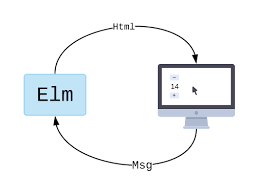
\includegraphics[width=.8\linewidth]{elm-arch-site}
\end{subfigure}%
\begin{subfigure}{.5\textwidth}
  \centering
  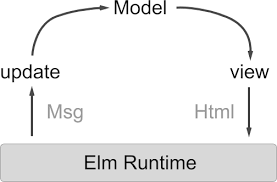
\includegraphics[width=.7\linewidth]{elm-arch-book}
\end{subfigure}
\caption{Arhitektura \emph{Elm}}
\label{fig:elm-arh}
\end{figure}

U levom delu slike \ref{fig:elm-arh} prikazano je kako radi svaki \emph{Elm} program: generiše
se \emph{HTML} koji se prikazuje u pretraživaču, nakon čega pretraživač šalje poruku programu
ukoliko se nešto dogodilo. U desnom delu slike vidimo šta se dešava unutar programa,
na osnovu primljene poruke funkcija \texttt{\textbf{update}} kreira novi\texttt{
\textbf{model}}, koji se prosleđuje funkciji \texttt{\textbf{view}}, na osnovu koje
se generiše \emph{HTML}.

Ovaj obrazac projektovanja ce često naziva i \emph{MVU} (eng. \emph{Model-View-Update}). Za 
razliku od obrazaca \emph{MVC} \cite{jsPatterns} (eng.\emph{Model-View-Controller}) i \emph{MVVM} \cite{jsPatterns}
(eng. \emph{Model-View-ViewModel}), koji stanje aplikacije dele na više manjih modela,
u arhitekturi \emph{Elm} celokupno stanje apikacije se nalazi na jednom mestu, tj. modelu, a
protok podataka kroz aplikaciju je uvek u jednom smeru. 

\emph{Arhitektura Elm} uticala je na nastajanje velikog broja biblioteka za upravljanje
stanjem veb aplikacije, među kojima su najpoznatije \emph{Redux}\cite{redux} i \emph{Vuex}\cite{vuex}.
Takođe, podrška za rad sa obrascem \emph{MVU} počinje da se pojavljuje i u drugim tehnologijama,
jedna od njih je i \emph{.NET 5} \cite{net5}.

\subsection{Generisanje HTML sadržaja}
Za razliku od drugih razvojnih okvira koji uglavnom koriste \emph{HTML} šablone (eng. \emph{templates}), \emph{Elm} za 
opisivanje izgleda stranice koristi funkcije. Stoga imamo funkcije za kreiranje \emph{HTML}
čvorova i atributa.
\begin{listing}[h]
  \begin{minted}{haskell}
  --   <button   id="btn-ok"  class="btn-default">    Ok      <\button>
  node "button" [id "btn-ok", class "btn-default"] [text "Ok"]
  -- korišćenje pomoćne funkcije button umesto node "button"
        button  [id "btn-ok", class "btn-default"] [text "Ok"]
  \end{minted}
  \caption{Primeri kreiranja \emph{HTML} čvorova}
  \label{listing:nodeHtml}
  \end{listing}
  
Funkcija \texttt{\textbf{node}} iz modula \texttt{\textbf{Html}} predstavlja generičku
funkciju za kreiranje \emph{HTML} čvorova, koja kao argumente prima \emph{HTML} oznaku, listu atributa
i listu čvorova (deca čvora). U primeru koda \ref{listing:nodeHtml} predstavljena je analogija
kreiranja \emph{HTML} čvora funkcijom \texttt{\textbf{node}} i \emph{HTML} sintakse.
Modul \texttt{\textbf{Html}} pruža veliki broj pomoćnih funkcija, koje imaju nazive po
\emph{HTML} oznakama (npr. \texttt{\textbf{button}} --- primer koda \ref{listing:nodeHtml}) i omogućavaju bolju čitljivost. Stoga se 
funkcija \texttt{\textbf{node}} koristi prilikom upotrebe korisnički definisanih elemenata
ili ukoliko ne postoji pomoćna funkcija za željeni element. Funkcija \texttt{\textbf{text}}
služi za postavljanje teksta u DOM, dok su \texttt{\textbf{id}} i \texttt{\textbf{class}}
funkcije za kreiranje atributa iz modula \texttt{\textbf{Html.Attributes}}.

\subsection{Elm program}
Prilikom inicijalizacije \emph{Elm} projekta se, pored paketa \texttt{\textbf{elm/core}} sa
osnovnim funkcionalnostima i strukturama podataka i paketa \texttt{\textbf{elm/html}} za
generisanje \emph{HTML} stranica, nalazi paket \texttt{\textbf{elm/browser}} za kreiranje \emph{Elm}
programa u pretraživaču. Unutar ovog paketa, u modulu \texttt{\textbf{Browser}} se nalaze
funkcije koje nam omogučavaju kreiranje različitih tipova programa, među kojima je i
funkcija \texttt{\textbf{sandbox}} namenjena za učenje osnova arhitekture \emph{Elm} i
omogućava bazičnu interakciju sa korisnicima, bez komunikacije sa spoljnim svetom.
Primer jednostavnog \emph{Elm} programa upotrebom funkcije \texttt{\textbf{sandbox}} prikazan
je u primer koda \ref{listing:elmProgram}.
\begin{listing}[h!]
\begin{minted}{haskell}
  module Main exposing (main)

  import Browser
  import Html exposing (Html, button, div, text)
  import Html.Events exposing (onClick)
  
  main =
    Browser.sandbox { init = init, update = update, view = view }

  --MODEL
  type alias Model = Int
  
  init : Model
  init =
    0
  
  -- UPDATE
  type Msg
    = Increment
    | Decrement
  
  update : Msg -> Model -> Model
  update msg model =
    case msg of
      Increment ->
        model + 1
  
      Decrement ->
        model - 1
  
  -- VIEW
  view : Model -> Html Msg
  view model =
    div []
      [ button [ onClick Decrement ] [ text "-" ]
      , div [] [ text (String.fromInt model) ]
      , button [ onClick Increment ] [ text "+" ]
      ]
\end{minted}
\caption{Primer \emph{Elm} programa}
\label{listing:elmProgram}
\end{listing}

Da bi okruženje \emph{Elm} znalo koja je polazna tačka programa potrebno je da se u glavnom
modulu definiše i izloži konstanta \textbf{\texttt{main}}, dok naziv modula nije bitan.
Pored funkcija iz modula \texttt{\textbf{Browser}}, u slučaju statičkih stranica, konstanta 
\textbf{\texttt{main}} se može definistati funkcijama iz modula \texttt{\textbf{Html}},
na primer: \mint{haskell}|main = text "Zdravo svete!"|

Da bi se pokrenuo program potrebno je pozicionirati se u komandnoj liniji na inicijalizovani
\emph{Elm} projekat i pokrenuti \texttt{\textbf{elm reactor}}. Nakon toga, potrebno je otvoriti pretraživač na
adresi \emph{http://localhost:8000} i unutar direktorijuma \texttt{\textbf{src}} kliknuti na 
\texttt{\textbf{Main.elm}} čime se vrši kompilacija i pokretanje programa. Takođe, primer se
može naći i na zvaničnom \emph{Elm} vodiču\cite{elm-program}. Na slici \ref{fig:brojac}
prikazan je izgled programa u pregledaču.
\begin{figure}[!ht]
  \centering
  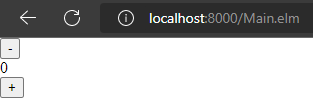
\includegraphics[width=0.5\textwidth]{brojac.png}
  \caption{Izgled programa u pregledaču}
  \label{fig:brojac}
\end{figure}

U primeru jednostavnog brojača iz primera koda \ref{listing:elmProgram} vidimo da funkcija
\textbf{\texttt{sandbox}} kao argument prima slog sa inicijalnom vrednošću modela i 
funkcijama za ažuriranje i prikazivanje modela. Program počinje pozivanjem funkcije
\texttt{\textbf{view}} sa parametrom \texttt{\textbf{init}}. Unutar funkcije
\texttt{\textbf{view}} se pomoću funkcije za kreiranje atributa iz modula
\texttt{\textbf{Html.Events}} mogu definisati načini slanja poruka, a kao rezultat 
izvršavanja nastaje virtuelni \emph{DOM}, na osnovu kog okruženje \emph{Elm} izmenjuje stvarni \emph{DOM}.
Ukoliko dođe do odgovarajuće akcije korisnika, u ovom sličaju klikom na dugme, okruženje \emph{Elm}
generiše poruku i prosleđuje je zajedno sa modelom funkciji \texttt{\textbf{update}} koja
kreira novi model nad kojim se poziva ponovo funkcija \texttt{\textbf{view}}.
Okruženje \emph{Elm} poredi prethodni virtuelni \emph{DOM} sa novim i vrši minimalan broj izmena.  

\chapter{Programski jezik Elixir}
Osnovne odlike jezika \emph{Elixir} sažete su u okviru njegove zvanične strane \cite{elixir}:
\begin{displayquote}
\emph{Elixir} je dinamički tipiziran, funkcionlni programski jezik dizajniran za izgradnju skalabilnih
aplikacija, lakih za održavanje.

\emph{Elixir} koristi virtuelnu mašinu programskog jezika \emph{Erlang}, poznatu po podršci za rad sistema sa malim kašnjenjem,
distribuiranih sistema i sistemima koji su otporni na greške, ali se uspešno koristi i u razvoju
veba, u sistemima sa ugrađenim računarom (eng. \emph{embedded sotfware}), učitavanju podataka
(eng. \emph{data ingestion}) i u domenima za obradu mulitmedije.
\end{displayquote}

Prva verzija programskog jezika \emph{Elixir} objavljena je 2011. godine. Autor jezika, Žozé Valim
(José Valim), prethodno je radio kao programer u programskom jeziku \emph{Ruby} i uvideo je probleme rada
razvojnog okvira \emph{Ruby on Rails} na višejezgarnim sistemima. Rešenje problema video je u novom funkcionalnom
programskom jeziku koji će koristiti prednosti virtuelne mašine jezika \emph{Erlang}. Stoga, najveći
uticaj na razvoj programskog jezika \emph{Elixir} imali su \emph{Erlang}, sa kojim je semantički vrlo sličan,
i \emph{Ruby} u smislu sintakse. 

\emph{Ruby} je dinamički tipiziran programski jezik opšte namene koji pruža mogućnost rada u više
programskih paradigmi. Nastao je sredinom devedesetih godina prošlog veka, a razvio ga je 
japanski naučnik i programer Jukihiro Macumoto (\emph{Yukihiro Matsumoto}). \emph{Ruby} je dizajniran
kao programski jezik fokusiran na programera, tako da svojom lakoćom korišćenja, jednostavnošću i 
fleksibilnošću učini programiranje prijatnijim. Sam autor kaže da pokušava da napravi \emph{Ruby} 
što prirodnijim.

Budući da je \emph{Elixir} nastao na ideji upotrebe virtuelne mašine jezika \emph{Erlang}, više o programskom jeziku \emph{Erlang} biće rečeno
u sledećem poglavlju. Takođe, pored dva navedena programska jezika, uticaj na razvoj \emph{Elixir}-a 
imali su \emph{Clojure} \cite{clojure}, \emph{Haskell}\cite{haskell} i \emph{Python}\cite{python}.

\section{Programski jezik i razvojna platforma Erlang}
\emph{Erlang} nije samo programski jezik, već i razvojna platforma za izgradnju skalabilnih i pouzdanih
sistema koji gotovo neprestano pružaju usluge. Švedska telekomunikaciona kompanija Erikson (eng.
\emph{Ericsson}) osmislila je ovu platformu sredinom osamdesetih godina prošlog veka. 
Da bi \emph{Erlang} mogao da upravlja telekomunikacionim sistemima kompanije, morao
je da bude pouzdan, skalabilan, da ima brz odziv i bude konstantno dostupan, jer telefonska mreža
mora da funkcioniše bez obzira na broj istovremenih poziva i neočekivane greške.

Iako je prvobitno izgrađen za telekomunikacione sisteme, \emph{Erlang} ni na koji način nije 
specijalizovan za ovaj domen, ne sadrži podršku za programiranje telefona i drugih 
telekomunikacionih uređaja. \emph{Erlang} predstavlja razvojnu platformu koja pruža posebnu podršku
tehničkim zahtevima kao što su: paralelnost, skalabilnost, tolerancija na
greške, distribuiranost i velika dostupnost. U vreme njegovog nastajanja, programi su se uglavnom
koristili bez komunikacije sa nekim veb servisom (eng. \emph{desktop-based sotfware}), pa je 
upotreba \emph{Erlang} jezika bila ograničena na telekomunikacione sisteme. Međutim, zahtevi modernih 
sistema i aplikacija poklapaju se sa tehničkim zahtevima za koje \emph{Erlang} pruža podršku, tako
da je u poslednje vreme privukao veliku pažnju. \emph{Erlang} pokreće razne velike sisteme, među kojima
su aplikacije \emph{WhatsApp}\cite{whatsapp} i \emph{WeChat}\cite{wechat},
distribuirana baza podataka \emph{Riak}\cite{riak} i \emph{Heroku Cloud}\cite{heroku}.

Kao razvojna platforma, \emph{Erlang} se sastoji od jezika, virtuelne mašine, razvojnog okvira (eng.
\emph{framework}) i alata.
\subsection{ Virtuelna mašina Erlang --- BEAM}
Jezik \emph{Erlang} predstavlja primaran način pisanja koda koji se izvršava na sopstvenoj virtuelnoj
mašini koja se naziva \emph{BEAM}. \emph{BEAM} je skraćenica za \emph{Bogdan’s Erlang Abstract Machine}, po
Bogumilu Bogdanu Hausmanu koji je kreirao originalnu verziju, ali se može posmatrati i kao
\emph{Björn’s Erlang Abstract Machine}, po Bjornu Gustavsonu koji održava trenutnu verziju 
virtuelne mašine. 

K\^{o}d napisan u programskom jeziku \emph{Erlang} se prevodi u binarni k\^{o}d (eng. \emph{bytecode})
koji se unutar \emph{BEAM}-a izvršava paralelno u vidu veoma lakih \emph{Erlang procesa}. \emph{BEAM}, umesto 
da se oslanja na procese i niti operativnog sistema, samostalno raspoređuje konkurentne
\emph{Erlang procese} na dostupna procesorska jezgra, što je prikazano na slici \ref{fig:beam}.
\begin{figure}[h]
  \centering
  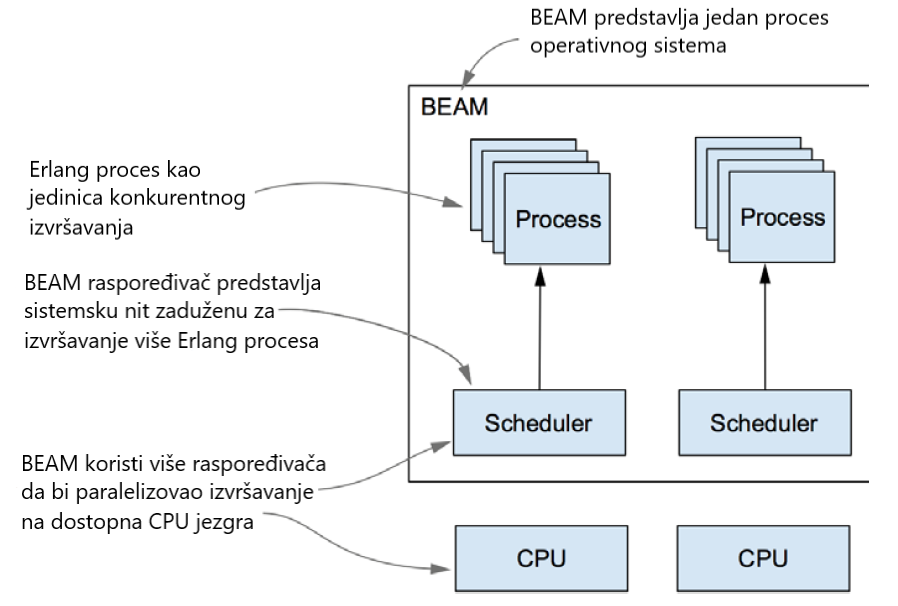
\includegraphics[width=0.6\textwidth]{beam.png}
  \caption{Način izvršavanja Erlang procesa unutar BEAM-a \cite{elixirInAction}}
  \label{fig:beam}
\end{figure}
Ovi laki procesi su međusobno potpuno izolovani, ne dele memoriju i komuniciraju preko
asinhronih poruka, što pruža mogućnost \emph{Erlang} sistemima da budu skalabilni, distribuirani i 
otporni na greške.  

\subsection{Razvojni okvir OTP}
\emph{OTP} je skraćenica za \emph{Open Telecom Platform}, što je donekle pogrešan naziv za ovaj razvojni
okvir. On nije vezan za telekomunikacione sisteme, već predstavlja razvojni okvir opšte namene koji
apstrahuje tipične zadatke \emph{Erlang} sistema:
\begin{itemize}
  \item Obrasce konkurentnosti i distribuiranosti
  \item Detekciju i oporavak od grešaka u konkurentnim sistemima
  \item Pravljenje biblioteka
  \item Postavljanje (eng. \emph{deployment}) sistema
  \item Uživo ažuriranje softvera 
\end{itemize}
\emph{OTP} predstavlja sastavni deo \emph{Erlang}-a, stoga i zvanična distribucija nosi naziv \emph{Erlang/OTP}.
\subsection{Odnos programskih jezika Erlang i Elixir}
\emph{Elixir} predstavlja alternativni način pisanja programa koji se izvršava na virtuelnoj
mašini BEAM i samim tim preuzima sve osobine platforme Erlang. Za razliku od Erlang-a pruža dodatne
koncepte koji omogućavaju značajno smanjenje ponavljajućeg i šablonskog (eng.
\emph{boilerplate}) koda. \emph{Elixir} i \emph{Erlang} su kompatibilni, pa \emph{Elixir} može direktno da koristi
\emph{Erlang} biblioteke i module. Važi i obrnuto, a sve što je moguće implementirati u programskom jeziku \emph{Erlang},
moguće je u programskom jeziku \emph{Elixir} bez razlike u performansama. Takođe, važno je napomenuti da oba jezika
odlikuje nepromenljivost podataka (imutabilnost).
\section{Uputstvo za instalaciju}
Proces instalacije je vrlo jednostavan, potrebno je pratiti uputstva sa zvanične \emph{Elixir}
stranice \cite{elixir} za odgovarajući operativni sistem. Podržani su gotovo svi operativni
sistemi. Provera usprešne instalacije može se izvršiti pokretanjem komande
\textbf{\texttt{elixir -{}-version}} u komandnoj liniji ili pokretanjem interaktivnog \emph{Elixir}-a
komandom \textbf{\texttt{iex}}.
\section{Osnovne odlike}
Za razliku od programskog jezika \emph{Elm}, \emph{Elixir} nije čist funkcionalni programski jezik, jer dozvoljava bočne efekte.
Pored prethodno spomenutih karakteristika preuzetih od \emph{Erlang}-a, dinamičke tipiziranosti i 
sintakse slične \emph{Ruby}-ju, \emph{Elixir} odlikuju izraženo poklapanje obrazaca, polimorfizam, makroi
i metaprogramiranje, kao i podrška za lenjo izračunavanje.
\section{Osnove jezika Elixir}
U ovoj glavi predstavljeni su osnovni operatori i tipovi podataka, poklapanje obrazaca,
definisanje i grupisanje funkcija u module. 
\subsubsection{Osnovni tipovi podataka}
Osnovne tipove podataka predstavljaju brojevi (celobrojni i realni), logičke
vrednosti, atomi i niske. Takođe, u osnovne tipove podataka jezika \emph{Elixir} ubrajaju se liste, torke i mape, ali će one biti objašnjene u poglavlju o strukturama podataka. Pregled
osnovnih tipova dat je u primeru koda \ref{listing:tipoviElixir}, gde se može videti i način pisanja
komentara. \emph{Elixir} podržava samo linijske komentare koji se označavaju simbolom \texttt{\textbf{\#}}.
\begin{listing}[!h]
\begin{minted}{elixir}
iex> 1          # integer
iex> 1.0        # float
iex> true       # boolean 
iex> :atom      # atom
iex> "elixir"   # string
\end{minted}
\caption{Pregled osnovnih tipova podataka u \emph{Elixir}-u}
\label{listing:tipoviElixir}
\end{listing}

\subsubsection{Celi brojevi}
Celi brojevi su još jedna razlika programskog jezika \emph{Elixir} u odnosu na \emph{Elm}
u smislu da nemaju ograničen opseg vrednosti. Takođe, pored
heksadecimalnog zapisa, \emph{Elixir} pruža mogućnost navođenja celobrojnih vrednosti u binarnom i 
oktalnom obliku. Simbol \texttt{\textbf{\textunderscore}} može se koristiti za odvajanje 
cifara i kod celih i kod brojeva u pokretnom zarezu (primer koda \ref{listing:brojeviElixir}).
\subsubsection{Brojevi u pokretnom zarezu}
Brojevi u pokretnom zarezu su dvostruke preciznosti (64 bita) i delimično prate
standard \emph{IEEE-754}, jer ne postoji podrška za vrednosti \texttt{NaN} i \texttt{Infinity}.
Vrednosti brojeva se mogu navoditi i u eksponencijalnom zapisu.
\begin{listing}[!h]
\begin{minted}{elixir}
iex> 10_000
10000
iex> 0o77
63
iex> 0b111_111
63
iex> 0xFF
255
iex> 1_000_000.000_123
1000000.000123
iex> 1.23e-3
0.00123
\end{minted}
\caption{Primeri celih i realnih brojeva u \emph{Elixir}-u}
\label{listing:brojeviElixir}
\end{listing}
\subsubsection{Atomi}
Atom je konstanta čiju vrednost predstavlja njeno ime. Definiše se dvotačkom (\texttt{\textbf{:}}),
nakon koje slede alfanumerički karakteri, simboli \texttt{\textbf{@}} ili 
\texttt{\textbf{\textunderscore}}, a može se završavati znakom pitanja ili uzvika. Takođe, moguće
je koristite i razmake, tada se sadržaj posle dvotačke mora navesti unutar navodnika.
Postoji i notacija atoma bez početne dvotačke, ali u tom slučaju moraju počinjati velikim
slovom, takvi atomi se nazivaju \emph{alijasi} i tokom kompilacije se transformišu u atome oblika
\texttt{:''Elixir.<naziv aliasa>''}. Upotreba atoma prikazana je u primeru koda \ref{listing:atomi}.

Atom se sastoji od teksta i vrednosti. U toku izvršavanja tekst se čuva u \emph{tabeli atoma},
dok vrednost predstavlja referencu na tekst u tabeli atoma, što omogućava brže poređenje atoma
kao i veću uštedu memorije. Obzirom da predstavljaju efikasan način za imenovanje konstanti,
atomi su svuda prisutni.
\begin{listing}[!h]
\begin{minted}{elixir}
iex> :neka_vrednost
:neka_vrednost
iex> :"atom sa razmacima"
:"atom sa razmacima"
iex> AliasAtom # kompilacijom se transformiše u :"Elixir.AliasAtom"
AliasAtom
iex> AliasAtom == :"Elixir.AliasAtom"
true
\end{minted}
\caption{Primeri atoma u \emph{Elixir}-u}
\label{listing:atomi}
\end{listing}
\paragraph{Logičke vrednosti kao atomi}
\emph{Elixir} zapravo nema poseban tip za logičke vrednosti, već koristi atome
\texttt{\textbf{:true}} i \texttt{\textbf{:false}}, i pruža mogućnost njihovog navođenja
bez početne dvotačke, tj. samo sa \texttt{\textbf{true}} i \texttt{\textbf{false}}.
\emph{Elixir} pruža funkcije za proveru tipa podataka, među kojima su \texttt{\textbf{is{\textunderscore}atom}} i \texttt{\textbf{is{\textunderscore}boolean}}
i čija upotreba je predstavljena u primeru koda \ref{listing:boolAtomi}.
\begin{listing}[!h]
\begin{minted}{elixir}
iex> is_atom(true)
true
iex> is_boolean(:true)
true
iex> false == :false
true
\end{minted}
\caption{Predstavljanje logičkih vrednosti preko atoma}
\label{listing:boolAtomi}
\end{listing}

Pored logičkih vrednosti, jos jedna specifična vrednost predstavljena atomom jeste
\texttt{\textbf{:nil}}, slična vrednosti \texttt{\textbf{null}} u drugim programskim jezicima.
Ona se takođe može navoditi bez početne dvotačke (sa \texttt{\textbf{nil}}).
\subsubsection{Niske}
Niske (\texttt{\textbf{string}}) se navode slično kao u \emph{Elm}-u, unutar jednostrukih ili trostrukih navodnika, s tim da se u slučaju trostrukih navodnika oni moraju navesti u posebnim redovima.
U \emph{Elixir}-u, niske koriste \emph{UTF-8} kodiranje i pružaju mogućnost ugrađivanja izraza --- interpolaciju
niski, što se može videti u primeru koda \ref{listing:elixirString}.
\begin{listing}[!h]
\begin{minted}{elixir}
iex> "Ćao!"
"Ćao!"
iex(1)> """
...(1)> Niska u više
...(1)> redova.
...(1)> """
"Niska u vise\nredova.\n"
iex> "1+1=#{1+1}"
"1+1=2"
\end{minted}
\caption{Primeri stringova u \emph{Elixir}-u}
\label{listing:elixirString}
\end{listing}
\paragraph{Niske bitova i sekvence bajtova}
Kao i kod logičkih vrednosti, \emph{Elixir} nema poseban tip za niske, već za njihovo
predstavljanje koristi sekvencu bajtova (eng. \emph{binary}) i \emph{UTF-8} kodiranje.
Zapravo fundamentalni tip za njihovo predstavljanje jeste niska bitova --- \textbf{bitstring}, kojoj odgovara neprekidni niz bitova u memoriji. Niske bitova mogu biti proizvoljne dužine, a sekvenca
bajtova ---\emph{binary} predstavlja posebnu vrstu niske bitova čiji je broj bitova deljiv sa
osam. 

Niske bitova se navode kao sekvenca brojeva unutar znakova
\texttt{\textbf{<\smallskip<}} i \texttt{\textbf{>\smallskip>}}. Podrazumevano se koristi
osam bitova za čuvanje svakog broja u bitstringu, ali je moguće navesti broj bitova pomoću
modifikatora \texttt{\textbf{::n}} da bi se označila veličina od \texttt{\textbf{n}} bitova,
ili u opširnijoj notaciji \texttt{\textbf{::size(n)}}.
\begin{listing}[!h]
\begin{minted}{elixir}
iex> is_binary(<<1,2>>)
true
iex> is_bitstring(<<1::1>>) # 1 bit
true
iex> is_binary(<<1::1,2>>) # 9 bitova
false
iex> <<1::1,0::1,1::1>>
<<5::size(3)>>
iex> is_binary("neki string")
true
iex> byte_size("Ćao") # Ć zauzima 2 bajta
4
iex> ?a # određivanje koda karakter a
97
iex> <<97,98,99>>  
"abc"
\end{minted}
\caption{Predstavljane nisk kao niz bajtova}
\label{listing:elixirBitstring}
\end{listing}
U primeru koda \ref{listing:elixirBitstring} vidimo da ukoliko sadržaj niske bitova čine samo ASCII
karakteri, interaktivni \emph{Elixir} ispisuje nisku. \emph{Elixir} nema tip \texttt{Char} za rad sa
karakterima, ali daje mogućnost određivanja koda pomoću simbola \texttt{\textbf{?}}, nakon 
kog se navodi karakter.

\subsubsection{Drugi ugrađeni tipovi podataka}
Pored navedenih, \emph{Elixir} poseduje i druge ugrađene tipove podataka:
\begin{itemize}
  \item Referenca --- jedinstven podatak u jednoj BEAM instanci i jedinstvenost je
  zagarantovana samo tokom životnog veka te instance
  \item Identifikator procesa (\emph{pid}) --- koristi se za identifikaciju \emph{Erlang} procesa
  \item Identifikator porta --- koristi se za identifikaciju porta, mehanizma koji se
  koristi za komunikaciju sa spoljnim svetom (datotekama, programima...)
\end{itemize} 

\subsection{Osnovni operatori}
Za razliku od \emph{Elm}-a, \emph{Elixir} vrši implicitnu konverziju celih brojeva u realne prilikom
primene aritmetičkih operatora \textbf{\texttt{+}}, \textbf{\texttt{-}} i
\textbf{\texttt{*}} ukoliko operandi nisu istog tipa, dok se u slučaju operatora
\textbf{\texttt{/}} ona uvek vrši, tako da je rezultat deljenja uvek realan broj. Za 
celobrojno deljenje i izračunavanje ostatka pri celobrojnom deljenju koriste se funkcije 
\textbf{\texttt{div}} i \textbf{\texttt{rem}}, koje se mogu koristiti samo nad celim brojevima.

Relacijski operatori u \emph{Elixir}-u slični su kao i u drugim jezicima. S tim što pored operatora 
\texttt{\textbf{==, !=, <=, >=, <}} i \texttt{\textbf{>}}, postoje i operatori 
\texttt{\textbf{===}} i \texttt{\textbf{!==}} koji se od operatora \texttt{\textbf{==}} i
\texttt{\textbf{!=}} razlikuju samo prilikom poređenja brojeva, tako što ne vrše konverziju
tipova, tj. vrše poređenje po tipu i vrednosti. Upotreba operatora poređenja prikazana je u
primeru koda \ref{listing:elixirOp}.
\begin{listing}[!h]
\begin{minted}{elixir}
iex> 1 == 1.0
true
iex> 1 === 1.0
false
iex> 1 == "1"
false
iex> 1 < false and "12" > '123'
true
\end{minted}
\caption{Rad sa operatorima poređenja}
\label{listing:elixirOp}
\end{listing}
Takođe, u primeru koda \ref{listing:elixirOp} vidimo da \emph{Elixir} dozvoljava poređenje vrednosti
različitih tipova i to po sledećem uređenju : \textbf{\texttt{number < atom < reference <
function < port < pid < tuple < map < list < bitstring}}

Logički operatori u \emph{Elixir}-u su specifični po tome što rezultat njihove primene ne mora
biti logička vrednost, već može biti vrednost proizvoljnog tipa. Takođe, \emph{Elixir} ima dvostruke operatore
za logičko \emph{i}, \emph{ili} i \emph{ne}, koji se mogu podeliti u dve grupe:
\begin{enumerate}
  \item \textbf{\texttt{and}}, \textbf{\texttt{or}} i \textbf{\texttt{not}} --- prvi operand
  mora biti logička vrednost
  \item \textbf{\texttt{\&\&}}, \textbf{\texttt{||}} i \textbf{\texttt{!}} --- oba operanda 
  mogu biti proizvoljnog tipa
\end{enumerate}
Operatori čiji operandi mogu biti proizvoljnog tipa zasnivaju se na konceptu istinitosti, gde
se vrednosti \textbf{\texttt{nil}} i \textbf{\texttt{false}} smatraju za lažne, a sve ostale
za istinite. Operatori su lenjo izračunljivi, tako da u slučaju primene operatora konjukcije
rezultat predstavlja drugi operand samo ako je prvi istinit ili se može smatrati istinitim
u slučaju operatora \texttt{\&\&}. Dok prilikom primene operatora disjunkcije rezultat je
prvi operand ukoliko je tačan ili se može smatrati tačnim (operator \texttt{||}), a u suprotnom vraća
se vrednost drugog operanda. Rad sa logičkim operatorima prikazan je u primeru koda
\ref{listing:elixirLogicOp}.
\begin{listing}[!h]
\begin{minted}{elixir}
iex> true and true
true
iex> false or 1
1
iex> not 1
** (ArgumentError) argument error
iex> !1
false
iex> nil && "bilo sta"
nil
iex> :atom || false
:atom
\end{minted}
\caption{Primeri upotrebe logičkih operatora}
\label{listing:elixirLogicOp}
\end{listing}

\subsection{Funkcije i moduli}
\emph{Elixir}, kao i \emph{Elm}, poseduje imenovane i anonimne funkcije. Imenovane funkcije se navode
isključivo unutar modula, a sintaksa je veoma jednostavna i prikazana je u primeru koda
\ref{listing:elixirModul}.
\begin{listing}[!h]
\begin{minted}{elixir}
defmodule Kalkulator do
  def pomnozi(x, y), do: x * y

  #privatna funkcija
  defp saberi(x, y) do 
    x + y
  end

  def saberi_i_ispisi(x, y) do
    IO.puts("#{a} + #{b} = #{a+b}")  #primer bočnog efekta
    saberi(x, y)
  end
end
\end{minted}
\caption{Primeri definisanja funkcija}
\label{listing:elixirModul}
\end{listing}

Za razliku od \emph{Elm}-a, gde funkcija predstavlja izvršavanje jednog izraza, u \emph{Elixir}-u
je moguće izvršiti više njih, a poslednji izraz predstavlja povratnu vrednost. U slučaju
jednog izraza unutar funkcije može se koristiti i skraćena sintaksa --- funkcija
\texttt{pomnozi} u primeru koda \ref{listing:elixirModul}, dok u funkciji
\texttt{saberi\textunderscore{}i\textunderscore{}ispisi} vidimo da je dozvoljeno pisanje
funkcija koje imaju bočne efekte. Ukoliko je predviđeno da se neke funkcije koriste samo
unutar modula, one se definišu kao privatne ključnom rečju \texttt{\textbf{defp}}.

Naziv modula mora počinjati velikim slovom i po konvenciji se pišu u kamiljoj notaciji, dok je 
imenovanje funkcija identično imenovanju promenljivih, s tim što funkcija čiji naziv se 
završava simbolom \texttt{\textbf{?}} po konvenciji vraća vrednosti \texttt{\textbf{true}} ili
\texttt{\textbf{false}}, a simbolom \texttt{\textbf{!}} se označava funkcija koja može izazvati
grešku prilikom izvođenja.
Pozivanje imenovanih funkcija moguće je sa i bez navođenja zagrada, dok su argumenti
razdvojeni zarezima. Na primer, funkciju \texttt{pomnozi} možemo pozvati sa:\\
\texttt{Kalkulator.pomnozi(2, 3)} i \texttt{Kalkulator.pomnozi 2, 3}.

\emph{Elixir}, nasuprot \emph{Elm}-u, nema ugrađene Karijeve funkcije, dozvoljava navođenje
podrazumevanih vrednosti, kao i preopterećivanje funkcija, što je i prikazano u primeru koda
\ref{listing:elixirOverload}. Funkciju potpuno određuje modul u kome se nalazi, naziv i
arnost (broj argumenata), tako da potpun naziv operatora nadovezivanja listi jeste
\emph{Kernel.++/2}. 
\begin{listing}[!h]
\begin{minted}{elixir}
defmodule Pravougaonik do
  def povrsina(a), do: a * a      # Pravougaonik.povrsina/1
  def povrsina(a, b), do: a * b   # Pravougaonik.povrsina/2
end

defmodule Brojac do
  # podrazumevana vrednost za n je 1 
  def uvecaj(x, n \\ 1), do: x + n
end
\end{minted}
\caption{Upotreba preopterećivanja funkcija i podrazumevanih vrednosti }
\label{listing:elixirOverload}
\end{listing}

Pored različitog broja argumenata, preopterećivanje funkcije
može se vršiti korišćenjem čuvara (eng. guards), tj. postavljanjem uslova nad argumentima
prilikom definisanja funkcija. Primer preopterećivanja funkcije upotrebom čuvara dat je u primeru koda
\begin{listing}[!h]
\begin{minted}{elixir}
defmodule Math do
  def sgn(x) when x < 0 do
    -1
  end
  
  def sgn(0), do: 0
  
  def sgn(x) when x > 0 do
    1
  end
end
\end{minted}
\caption{Preopterećivanja funkcija upotrebom čuvara}
\label{listing:elixirOverload}
\end{listing}

\subsubsection{Anonimne funkcije}
Sintaksa navođenja anonimnih funkcija prikazana je u primeru koda \ref{listing:elixirLambda}. Za
razliku od imenovanih funkcija, argumenti se ne navode unutar zagrada po konvenciji, mada je
moguće koristiti zagrade. Takođe, prilikom pozivanja anonimnih funkcija obavezno je korišćenje
zagrada i navođenje tačke (\texttt{\textbf{.}}) pre njih. 
\begin{listing}[!h]
\begin{minted}{elixir}
iex> saberi = fn x, y ->
...>  x + y
...> end
saberi.(1, 2)
3
\end{minted}
\caption{Primer definisanja i pozivanja anonimne funkcije}
\label{listing:elixirLambda}
\end{listing}

Anonimne (lambda) funkcije u \emph{Elixir}-u se razlikuju od imenovanih i ubrajaju se u osnovne tipove
podataka. Imenovane funkcije nije moguće proslediti kao parametar ili vezati za promenljivu,
već se za to mogu korisiti isključivo anonimne funkcije. Ovaj nedostatak imenovanih funkcija se može prevazići upotrebom
operatora \texttt{\textbf{\&}} (eng. \emph{capture}), koji imenovanu funkciju pretvara u
anonimnu. Operator \texttt{\textbf{\&}} se može koristiti i za kraću sintaksu anonimnih funkcija,
što je i prikazano u primeru koda \ref{listing:elixirCapture}.
\begin{listing}[!h]
\begin{minted}{elixir}
iex> saberi1 = &Kernel.+/2
iex> saberi1.(3, 4)
7
iex> saberi2 = &(&1 + &2) # &n je n-ti argument
iex> saberi2.(5, 6)
11
\end{minted}
\caption{Primer upotrebe \texttt{\textbf{\&}} operatora}
\label{listing:elixirCapture}
\end{listing}

Zatvorenja (eng. \emph{closures}) predstavljaju još jednu specifičnost lambda funkcija u
\emph{Elixir}-u. Prilikom definisanja, lambda funkcija ima pristup svim vrednostima unutar opsega u
kom se definiše. Ukoliko koristi vrednosti promenljivih van svog opsega, kreiraju se reference na trenutne
vrednosti promenljivih i ponovno vezivanje promenljivih ne utiče na izvršavanje funkcije. U
primeru koda \ref{listing:elixirClosures} dat je primer zatvorenja.
\begin{listing}[!h]
\begin{minted}{elixir}
iex> x = 3
3
iex> saberi_sa_3 = &(&1 + x)
iex> saberi_sa_3.(3)
6
iex> x = 4
4
iex(35)> saberi_sa_3.(3)
6
\end{minted}
\caption{Primer zatvorenja u \emph{Elixir}-u}
\label{listing:elixirClosures}
\end{listing}
 
\subsubsection{Operator prosleđivanja - \emph{pipe} operator (\texttt{\textbf{|>}})}
Operator \texttt{\textbf{|>}} u \emph{Elixir}-u prosleđuje vrednost sa leve strane kao prvi argument
funkciji sa desne strana, što je različito ponašanje koje isti operator ima u \emph{Elm}-u, gde se
vrednost sa leve strane prosleđuje kao poslednji argument funkciji sa desne
strane. Takođe, \emph{Elixir} ne podržava slične operatore koji postoje u \emph{Elm}-u. Različito ponašanje
operatora \texttt{\textbf{|>}} u oba jezika predstavljeno je u primeru koda \ref{listing:elixirPipe}.
\begin{figure}[!h]
\begin{minipage}{0.5\textwidth}
  \centering
  \begin{minted}{elixir}
    iex> podeli = &(&1 / &2)
    iex> 1 |> podeli.(2)
    0.5
  \end{minted}
\end{minipage}
\begin{minipage}{0.5\textwidth}
  \centering
  \begin{minted}{haskell}
    > podeli x y = x / y
    > 1 |> podeli 2
    2 : Float
  \end{minted}
\end{minipage}
\captionof{listing}{Upotreba \textbf{pipe} operatora u \emph{Elixir}-u (levo) i \emph{Elm}-u (desno)}
\label{listing:elixirPipe}
\end{figure}

\subsubsection{Atributi}
Atributi u modulu se mogu koristiti za definisanje konstanti. Takođe, \emph{Elixir} pruža atribute
za dokumentovanje koda: \texttt{@moduledoc} i \texttt{@doc}, čija je upotreba prikazana u
primeru koda \ref{listing:elixirAtributi}.
\begin{listing}[!h]
\begin{minted}{elixir}
defmodule Krug do
  @moduledoc "Osnovne funkcije za rad sa krugovima"
  #definisanje konstante
  @pi 3.141593 

  @doc "Izračunava obim kruga"
  def obim(r), do: 2*r*@pi

  @doc "Izračunava povrsinu kruga"
  def povrsina(r), do: r*r*@pi
end
\end{minted}
\caption{Definisanje konstante i dokumentovanje koda pomoću atributa}
\label{listing:elixirAtributi}
\end{listing}
Atributi imaju višestruku upotrebu i mnogi bitni koncepti se zasnivaju na njima, među kojima
je i specifikacija tipova (eng. \emph{typespecs}) koja se može koristiti za definisanje
korisničkih tipova, kao i za anotaciju tipova sličnu anotaciji u \emph{Elm}-u. Više o specifikaciji
tipova i samim atributima može se videti na zvaničnoj stranici \cite{elixir}.

\subsubsection{Korišćenje funkcija iz drugog modula}
Funkcije modula mogu se pozivati kao \emph{NazivModula.naziv\textunderscore{}funkcije},
što često nije praktično jer nazivi modula
mogu biti veoma dugački. Stoga \emph{Elixir} nudi dve direktive za kraći i čitljiviji k\^{o}d prilikom
upotrebe funkcija iz drugih modula --- \texttt{import} i \texttt{alias}, koje su prikazane u
primeru koda \ref{listing:elixirAliasImport}.

Upotrebom direktive \texttt{import} sve funkcije navedenog modula uključuju se u trenutni
modul i mogu se pozivati bez navođenja imena modula, a moguće je ograničiti uključivanje samo
određenih funkcija. Sa druge strane, \texttt{alias} omogućava korišćenje određenog imena
(alijasa) za bilo koji modul i prilikom pozivanja funkcija obavezno je njegovo navođenje.
\begin{listing}[h]
\begin{minted}{elixir}
alias Api.Accounts.User, as: AccUser
alias Api.Accounts.User #isto kao alias Api.Accounts.User, as: User

# uključivanje samo authenticate/2 funkcija 
import Api.Accounts, :only [authenticate: 2] 
\end{minted}
\caption{Upotreba direktiva \texttt{import} i \texttt{alias}}
\label{listing:elixirAliasImport}
\end{listing}

\subsection{Osnovne strukture podataka}
Osnovne strukture podataka u programskom jeziku \emph{Elixir} predstavljaju liste, torke i mape.
Pored njih, bitno mesto zauzimaju i liste ključnih reči. Podaci u \emph{Elixir}-u su nepromenljivi (imutabilni) i prilikom izvršavanja operacija nad njima ne menja se trenutna vrednost, već se uvek
kreira nova.

\subsubsection{Liste}
Kao i u \emph{Elm}-u, lista kao tip predstavlja jednostuko povezanu listu, čiji se elementi navode
unutar uglastih zagrada, ali za razliku od \emph{Elm}-a ne moraju biti istog tipa. U modulu \texttt{\textbf{Kernel}} se nalaze operatori za proveru da li element pripada listi
(\texttt{\textbf{in}}), za nadovezivanje listi (\texttt{\textbf{++}}), kao i operator oduzimanja
(\texttt{\textbf{-{}-}}) koji predstavlja razliku elemenata levog i desnog operanda. Tu su i funkcije
za određivanje glave, repa i dužine liste. Umesto operatora \emph{cons}, \emph{Elixir} pruža sintaksu
u obliku \texttt{\textbf{[}glava\textbf{|}rep\textbf{]}} koja se može koristiti u kreiranju nove
liste i poklapanju obrazaca. Za rad sa listama može se koristiti veliki broj funkcija iz modula
\texttt{\textbf{List}}, kao i funkcije iz modula \texttt{\textbf{Enum}} o kom će više rečeno kasnije. Primeri upotrebe nekih od navedenih funkcija prikazani su u primeru koda \ref{listing:elixirList}.
\begin{listing}[h]
\begin{minted}{elixir}
iex> [1,2,3, "123", true] ++ [:atom, ["aaa", "bbb"]]
[1, 2, 3, "123", true, :atom, ["aaa", "bbb"]]
iex> [1, 2, 1, 3, 5] -- [1, 5, 6]
[2, 1, 3]
iex> "abc" in [1, 2, "abc", false]
true
iex> List.insert_at([0,1,2], 1, 3)
[0, 3, 1, 2]
iex> tl([1,2,3,4])
[2, 3, 4]
\end{minted}
\caption{Rad sa listama u \emph{Elixir}-u}
\label{listing:elixirList}
\end{listing}
\paragraph{Liste karaktera }
Lista karaktera (eng. \emph{charlists}) je lista celih brojeva, gde svaki element predstavlja jedan karakter.
Veoma je slična niskama, za navođenje se koriste apostrofi umesto navodnika, 
ali glavna razlika je u internoj reprezentaciji, kao i funkcijama koje se nad njima
izvršavaju. Mogu se navoditi u jednostrukoj i trostrukoj notaciji, a moguća je i 
interpolacija. U primeru koda \ref{listing:elixirCharList} dati su primeri liste karaktera.
\begin{listing}[h]
\begin{minted}{elixir}
iex>'''
Primer u
više redova
'''
'Primer u\nvise redova\n'
iex>'2+2=#{2+2}'
'2+2=4'
iex> [97,98,99]
'abc'
iex> '123' ++ [0] 
[49, 50, 51, 0]
\end{minted}
\caption{Primeri lista karaktera u \emph{Elixir}-u}
\label{listing:elixirCharList}
\end{listing}

\subsubsection{Torke}
I u \emph{Elixir}-u torke mogu sadržati elemente različitih tipova, ali za razliku od \emph{Elm}-a,
navode se unutar vitičastih zagrada, broj elemenata nije ograničen i elementi se mogu uklanjati
i dodavati. Iako dozvoljavaju promenljiv broj elemenata, torke su zamišljene kao kolekcija
podataka fiksne dužine. U modulu \texttt{\textbf{Kernel}}
se nalaze funkcije za pristupanje i ažuriranje elemenata, kao i funkcija za određivanje broja
elemenata torke, dok se ostale funkcije za rad sa torkama nalaze u modulu \texttt{\textbf{Tuple}}.
Prikaz rada navedenih funkcija dat je u primeru koda \ref{listing:elixirTorke}.
\begin{listing}[!h]
\begin{minted}{elixir}
iex> tuple_size({1, "aaa", false})
3
iex> elem({:prvi, :drugi, :treci}, 0)
:prvi
iex> put_elem({1, 2}, 1, 4)
{1, 4}
iex> Tuple.insert_at({1, 2}, 1, 4)
{1, 4, 2}
iex> Tuple.to_list({1, 2, 3})
[1, 2, 3]
\end{minted}
\caption{Rad sa torkama u \emph{Elixir}-u}
\label{listing:elixirTorke}
\end{listing}

\subsubsection{Liste ključnih reči}
Liste ključnih (eng. \emph{keyword list}) reči predstavljaju posebnu vrstu listi gde je svaki element dvočlana torka,
čiji je prvi član (tj. ključna reč) obavezno atom, a drugi može biti bilo kog tipa. Takođe,
jedna ključna reč može se navesti više puta. \emph{Elixir} pruža i jednostavniju sintaksu koja izuzima
pisanje vitičastih zagrada. Za rad sa listama ključnih reči mogu se koristiti sve funkcije i
operatori kao i sa običnim listama i, dodatno, funkcije iz modula \texttt{Keyword} i operator
\texttt{\textbf{[\smallskip]}} za prisup po određenoj ključnoj reči. Prikaz nekih od funkcija i operatora dat je u primeru koda \ref{listing:keywordList}.
\begin{listing}[!h]
\begin{minted}{elixir}
iex> [{:prvi, 1}, {:drugi, 2}, {:treci, 3}]
[prvi: 1, drugi: 2, treci: 3]
iex> Keyword.get([prvi: 1, drugi: 2, treci: 3], :drugi)
2
iex> lista = [prvi: 1, drugi: 2, treci: 3]
[prvi: 1, drugi: 2, treci: 3]
iex> lista[:prvi]
1
iex> [a: 1, b: 2] ++ [c: "3"]
[a: 1, b: 2, c: "3"]
\end{minted}
\caption{Primeri rada sa listama ključnih reči u \emph{Elixir}-u}
\label{listing:keywordList}
\end{listing}

\subsubsection{Mape}
Za razliku od liste ključnih reči, mape predstavljaju kolekciju elemenata u obliku
\emph{ključ-vrednost} gde oba člana mogu biti proizvoljnog tipa. Liste ključnih
reči čuvaju uređenje, što je osobina koju nemaju mape, ali u slučaju većeg broja elemenata
mape pružaju bolju efikasnost. Takođe, ključevi unutar mape moraju biti jedinstveni.
Elementi mape navode se koristeći \texttt{\textbf{\%\{\}}} sintaksu, a ključ i vrednost se
odvajaju znakom \texttt{\textbf{=>}}. U slučaju da su svi ključevi atomi, može se koristiti
jednostavnija sintaksa kao kod liste ključnih reči. Oba slučaja prikazana su u primeru koda 
\ref{listing:elixirMap}.
\begin{listing}[!h]
\begin{minted}{elixir}
iex> %{1 => false, "bb" => [1,2], {1,2} => 3}
%{1 => false, {1, 2} => 3, "bb" => [1, 2]}
iex> %{a: 123, b: 'bbb', c: "c"}
%{a: 123, b: 'bbb', c: "c"}
\end{minted}
\caption{Primeri mapa u \emph{Elixir}-u}
\label{listing:elixirMap}
\end{listing}

Pristup elementima mape moguć je pomoću operatora \texttt{\textbf{[\smallskip]}}, kao i
funkcija iz modula \texttt{Map}, a ukoliko su svi ključevi mape atomi, dostupna je 
sintaksa oblika \emph{mapa.ključ}. Pored funkcija iz modula \texttt{Map}, nad mapama se
mogu koristiti i funkcije iz modula \texttt{Enum}.
Mape predstavljaju dinamičku strukturu u kojoj se mogu dodavati i uklanjati elementi,
a moguće je i ažuriranje elemenata. Pored funkcija iz modula, dostupna je i sintaksa ažuriranja slična sintaksi ažuriranja slogova u \emph{Elm}-u i prikazana je u primeru koda \ref{listing:elixirMap2}.
\begin{listing}[!h]
\begin{minted}{elixir}
iex> mapa = %{a: 1, b: 2, c: 3}
%{a: 1, b: 2, c: 3}
iex>mapa.b
2
iex> mapa[:c]
3
iex> %{mapa | a: 4}
%{a: 4, b: 2, c: 3}
iex>%{ %{"a" => true, :b => 0} | :b => false}
%{:b => false, "a" => true}
\end{minted}
\caption{Pristup i ažuriranje elemenata mape}
\label{listing:elixirMap2}
\end{listing}

\subsubsection{Modul Enum}
\emph{Elixir} pruža koncept nabrojivih podataka (eng. \emph{enumerables}), odnosno tipove podataka
kroz koje je moguće iterirati. Veliki broj funkcija uobičajenih za ovaj tip podataka (pronalazak i transformisanje elemenata, grupisanje, sortiranje, filtriranje...) nalazi se u modulu \texttt{Enum}. Liste i mape spadaju u nabrojive tipove, a pored njih, \emph{Elixir} omogućava i rad sa \emph{opsezima} (eng. \emph{ranges}).
Upotreba  nekih od funkcija iz modula \texttt{Enum} nad listama, opsezima i mapama se može videti u primeru koda \ref{listing:elixirEnum}. Funkcije iz modula \texttt{Enum}
mogu raditi sa bilo kojim tipom koji implementira \texttt{Enumerable} protokol. Više
o protokolima biće rečeno u poglavlju 3.10.
\begin{listing}[!ht]
\begin{minted}{elixir}
iex> Enum.map([1, 2, 3], fn x -> x * 3 end)
[3, 6, 9]
iex> Enum.reduce(%{1 => 2, 3 => 4}, 0, fn {k, v}, s -> s + k + v end)
10
iex> Enum.filter(1..10, fn x -> rem(x, 3) == 0 end)
[3, 6, 9]
\end{minted}
\caption{Upotreba funkcija iz modula \texttt{Enum} nad listama, mapama i opsezima}
\label{listing:elixirEnum}
\end{listing}
\paragraph{Skraćenice}
Filtriranje i mapiranje nad nabrojivim podacima predstavljaju čestu pojavu u \emph{Elixir} programima,
te su uvedene skraćenice (eng. \emph{comprehensions}) kao sintaksička olakšica (eng. \emph{syntactic sugar}), koja
grupiše ovakve operacije u specijalnu formu koja se naziva \texttt{\textbf{for}}. Upotreba skraćenica
prikazana je u primeru koda \ref{listing:elixirComprehensions}, a više o njima može se pronaći na zvaničnoj
\cite{elixir} stranici.
\begin{listing}[!ht]
\begin{minted}{elixir}
for n <- 1..5, do: n * n
[1, 4, 9, 16, 25]
iex> for i <- [:a, :b, :c], j <- [1, 2], do:  {i, j}
[a: 1, a: 2, b: 1, b: 2, c: 1, c: 2]
iex> nije_paran? = &(rem(&1, 2) != 0)
iex> for n <- 1..10, nije_paran?.(n), do: 2 * n
[2, 6, 10, 14, 18]
\end{minted}
\caption{Primeri upotrebe skraćenica}
\label{listing:elixirComprehensions}
\end{listing}
\subsubsection{Tokovi}
Tokovi (eng. \emph{Streams}) predstavljaju posebnu vrstu nabrojivih tipova koji se mogu koristiti za kreiranje
složenih lenjih operacija nad nabrojivim podacima. Tokovi su definisani u modulu
\texttt{Stream} i funkcije unutar ovog modula izgledaju vrlo slično funkcijama u modulu
\texttt{Enum}, s tim da je povratna vrednost ovih funkcija uvek tok, što omogućava
njihovu kompoziciju. Primer lenjog izračunavanja upotrebom tokova dat je u primeru koda
\ref{listing:elixirStream}. 
\begin{listing}[!ht]
\begin{minted}{elixir}
# kompozicija operacija, ne vrši se izračunavanje
iex> stream = 1..1_000_000 |> 
...> Stream.filter(&(rem(&1, 3) == 0)) |> 
...> Stream.map(&(&1 * 2))
# lenjo izračunavanje - samo za prvih 5
iex> stream |> Enum.take(5) 
[6, 12, 18, 24, 30]
\end{minted}
\caption{Kompozicija tokova i lenjo izračunavanje}
\label{listing:elixirStream}
\end{listing}

\subsection{Strukture}
Strukture predstavljaju koncept razvijen na osnovu mapa, s tim što imaju podrazumevane 
vrednosti, a ključevi su isključivo atomi. Sintaksa definisanja struktura data je u primeru koda
\ref{listing:elixirStruct}. Mogu se navoditi samo unutar modula i to najviše jedna.
\begin{listing}[!h]
\begin{minted}{elixir}
defmodule Osoba do
  defstruct ime: "Pera", godine: 25
end

defmodule Osoba1 do
  defstruct [:ime, godine: 25]
end
\end{minted}
\caption{Primeri definisanja struktura}
\label{listing:elixirStruct}
\end{listing}

Ukoliko se postavljaju podrazumevane vrednosti svih ključeva, moguće je izostaviti navođenje
uglastih zagrada. U suprotnom obavezno je njihovo koršćenje, pri čemu se nenavedenim ključevima
podrazumevana vrednost postavlja na \texttt{nil}. U slučaju da se nekim ključevima ne dodeljuje
podrazumevana vrednost, takvi ključevi se obavezno navode na početku liste. Sintaksa kreiranja
modula je slična sintaksi kreiranja mapa --- \texttt{\textbf{\%\emph{NazivModula}\{\}}}. U 
primeru koda \ref{listing:elixirStruct1} može se videti kreiranje stuktura iz primeru koda
\ref{listing:elixirStruct}.
\begin{listing}[!h]
\begin{minted}{elixir}
iex> %Osoba{}
%Osoba{godine: 25, ime: "Pera"}
iex> %Osoba1{}
%Osoba{godine: 25, ime: nil}
#moguće je specifikacija ključeva tokom kreiranja
iex> %Osoba1{godine: 30}
%Osoba1{godine: 30, ime: nil}
\end{minted}
\caption{Primeri kreiranja struktura}
\label{listing:elixirStruct1}
\end{listing}

Nad strukturama se mogu koristiti funkcije iz modula \texttt{Map}, ali ne i funkcije iz
modula \texttt{Enum}, kao ni operator \texttt{\textbf{[\smallskip]}}. Za pristup ključevima
koristi se isključivo sintaksa \emph{struktura.ključ}, a ažuriranje vrednosti može se izvršiti
korišćenjem simbola \texttt{\textbf{|}} kao kod mapa. Svaka struktura ima specijalni ključ 
\texttt{\textunderscore\textunderscore{}struct\textunderscore\textunderscore} koja sadrži 
naziv strukture, odnosno modula. 


\subsection{Poklapanje obrazaca}
U prethodnom poglavlju nije naveden jedan od najvažnijih operatora u programskom jeziku
\emph{Elixir} --- operator uparivanja ili poklapanja (\texttt{\textbf{=}}), koji ima veoma
bitnu ulogu u poklapanju obrazaca. Za razliku od \emph{Elm}-a gde se
poklapanje obrazaca korisiti isključivo unutar izraza \textbf{\texttt{case}} i
\textbf{\texttt{let}}, u \emph{Elixir}-u je ono dosta prisutnije i koristi se prilikom
definisanja promenljivih i funkcija, kao i u kontroli toka.

Operator uparivanja pokušava da izraz sa leve strane upari sa izrazom sa desne strane,
ukoliko ne dođe do uspešnog uparivanja prijavljuje grešku --- \texttt{MatchError}.
U većini drugih programskih jezika, operator \texttt{\textbf{=}} koristi se za dodeljivanje
vrednosti promenljivoj, što se u \emph{Elixir}-u postiže kroz poklapanje obrazaca. Ukoliko
dođe do uspešnog poklapanja, promenljive u levom izrazu \emph{vezuju se} za odgovarajuće
vrednosti u desnom. Imenovanje promenljivih slično je imenovanju atoma, s tim što umesto
dvotačke promenljiva mora počinjati malim slovom, po konvenciji se koristi
\emph{snake\textunderscore{}case} notacija. Moguće je koristiti operator uparivanja bez 
promenljivih, kao i izvršiti ponovno vezivanje promenljive za drugu vrednost, što je 
prikazano u primeru koda \ref{listing:elixirPoklapanjeObrazaca}. Takođe, ukoliko ne želimo
ponovno vezivanje možemo korisiti \emph{pin} operator \textbf{\texttt{ \^{}}}.
\begin{listing}[!h]
\begin{minted}{elixir}
iex> x = 1
1
iex> 1 = 1
1
iex> x = x + 1
2
iex> 1 = x  
** (MatchError) no match of right hand side value: 2
iex> ^x = 1
** (MatchError) no match of right hand side value: 1
\end{minted}
\caption{Vezivanje promenljive za vrednost}
\label{listing:elixirPoklapanjeObrazaca}
\end{listing}

Operator uparivanja se često upotrebljava za pristupanje elementima torki, listi i mapa,
gde se može izvršiti vezivanje više promenljivih odjednom. Kao i u \emph{Elm}-u, simbol 
\texttt{\textbf{\textunderscore}} se može koristiti za poklapanje vrednosti koje se neće
dalje koristiti. Primeri poklapanja obrazaca listi i torki dati su u primeru koda
\ref{listing:elixirPoklapanjeTorki}.
\begin{listing}[!h]
\begin{minted}{elixir}
iex> {a, b} = {1, 2}
{1, 2}
iex> [c, c] = [3, 3]
[3, 3]
iex> {1, 2, 3, d} = {a, b, c, {4}}
{1, 2, 3, {4}}
iex> [ _ | rep ] = 'abcd'
iex> rep
'bcd'
\end{minted}
\caption{Poklapanje obrazaca listi i torki}
\label{listing:elixirPoklapanjeTorki}
\end{listing}

U slučaju mapa moguće je parcijalno poklapanje, tj. leva strana ne mora da sadrži sve
ključeve desne, što omogućava pristupanje samo potrebnim vrednostima iz mape. Parcijalno
poklapanje je prikazano u primeru koda \ref{listing:elixirPoklapanjeMapa}.
\begin{listing}[!h]
\begin{minted}{elixir}
iex> %{ime: ime, godine: godine} = %{ime: "Pera", godine: 25}
%{godine: 25, ime: "Pera"}
iex> "#{ime} ima #{godine} godina."
"Pera ima 25 godina."
iex> %{ime: ime} = %{ime: "Pera", godine: 25}
%{godine: 25, ime: "Pera"}
iex(55)> %{ime: ime, prezime: prezime} = %{ime: "Pera", godine: 25}
** (MatchError) no match of right hand side value: %{godine: 25, ...
\end{minted}
\caption{Poklapanje obrazaca mapa}
\label{listing:elixirPoklapanjeMapa}
\end{listing}

Prilikom definisanja funkcija može se koristi poklapanje obrazaca za razlaganje argumenata,
ali i za preopterećivanje funkcija iste arnosti koršćenjem različitih šablona.
Primer preopterećivanja funkcije upotrebom poklapanja obrazaca dat je u primeru koda
\ref{listing:elixir-fn-pattern-matching}.
\begin{listing}[!h]
\begin{minted}{elixir}
defmodule Oblik do
  def povrsina({:pravougaonik, a, b}), do: a * b
  def povrsina({:kvadrat, a}), do: a * a
  def povrsina({:krug, r}), do: r * r * 3.141593
  # podrazumvani slučaj
  def povrsina(oblik), do: {:error, {:nepoznat_oblik, oblik}}
end
\end{minted}
\caption{Preopterećivanje funkcija upotrebom poklapanja obrazaca}
\label{listing:elixir-fn-pattern-matching}
\end{listing}

\subsection{Makroi}
Makroi predstavljaju jednu od najvažnijih novouvedenih karakteristika \emph{Elixir}-a u odnosu na \emph{Erlang}.
Makroi omogućavaju metaprogramiranje, tj. pisanje koda koji generiše k\^{o}d, što dovodi do 
značajnog smanjenja količine šablonskog (eng. \emph{boilerplate}) koda, a samim tim i do
vrlo čitljivog i elegantnog koda. Upotrebom makroa se tokom kompilacije vrše transformacije
nad kodom, čime se ne utiče na performanse izvršavanja. Makroi i metaprogramiranje nisu predmet
ovog rada, ali je neophodno razumeti kako makroi funkcionišu, jer su mnoge funkcionalnosti
\emph{Elixir}-a implementirane pomoću njih i njihova upotreba je gotovo neizbežna. 

Makroi se definišu unutar modula. Pre upotrebe, budući da se prevode tokom kompilacije, moduli
u kojima su definisani moraju biti dostupni, što se obezbeđuje direktivom \texttt{require}. 

Veoma bitan makro koji se često povezuje sa direktivama jeste makro \texttt{\textbf{use}},
koji omogućava ubacivanje spoljne funkcionalnosti (koda) u trenutni modul. U primeru koda 
\ref{listing:use} prikazan je primer upotrebe makroa \texttt{\textbf{use}} za kreiranje modula
sa jediničnim testovima pomoću biblioteke \emph{ExUnit}, koja je instalirana zajedno sa \emph{Elixir}-om.
\begin{listing}[h]
\begin{minted}{elixir}
defmodule ModulSaTestom do
  use ExUnit.Case

  test "uvek prolazi" do
    assert true
  end
end
\end{minted}
\caption{Upotreba makroa \texttt{use}}
\label{listing:use}
\end{listing}


\subsection{Kontrola toka}
\emph{Elixir} nema izraze ili naredbe za kotrolu toka i prethodno je prikazano kako
se korišćenjem čuvara i poklapanja obrazaca može vršiti kontrola toka izvršavanja.
Ovakva rešenja nisu uvek adekvatna i jednostavna za upotrebu,
jer podrazumevaju kreiranje zasebnih funkcija i prosleđivanje neophodnih
argumenata što dovodi do povećanja šablonskog (eng. \emph{boilerplate}) koda.
Stoga \emph{Elixir} uvodi makroe koji ovo rade tokom kompilacije umesto nas, i to su
\texttt{if, unless, cond} i \texttt{case}.

\subsubsection{Upotreba makroa \texttt{\textbf{if}} i \texttt{\textbf{unless}}}
Makro \texttt{if} se koristi za standardno \emph{if-else} grananje. Makro \texttt{unless} suprotan
je makrou \texttt{if} i može se posmatrati kao \texttt{if not}. Sintaksa upotrebe oba makroa data je
u primeru koda \ref{listing:elixirIf}. 
\begin{figure}[!h]
\begin{minipage}{0.5\textwidth} 
  \raggedleft 
  \begin{minted}{elixir}
    if uslovni_izraz do
        blok_izraza_1
    else
        blok_izraza_2
    end
  \end{minted}
\end{minipage}
\begin{minipage}{0.5\textwidth}
  \raggedright
  \begin{minted}{elixir}
    unless uslovni_izraz do
        blok_izraza_2
    else
        blok_izraza_1
    end
  \end{minted}
\end{minipage}
\captionof{listing}{Sintaksa makroa \texttt{if} i \texttt{unless}}
\label{listing:elixirIf}
\end{figure}
  
Kao kod operatora \texttt{\&\&} i \texttt{||} uslovni izraz se smatra tačnim ukoliko njegova
vrednost nije \texttt{nil} ili \texttt{false}. Za razliku od Elm-a, gde je navođenje \texttt{else}
grane obavezno, u \emph{Elixir}-u to nije slučaj. Vrednost izraza odgovara vrednosti poslednjeg
izraza u bloku, a ukoliko se \texttt{else} grana ne navede i uslov
nije istinit (odnosno nije neistinit u slučaju makroa \texttt{unless}), vrednost izraza je
\texttt{nil}. Postoje i skraćene, jednolinijske verzije sintaksi i prikazane su u primeru koda
\ref{listing:elixirShortIf}.
\begin{listing}[h]
\begin{minted}{elixir}
if uslovni_izraz, do: izraz_1, else: izraz_2

unless uslovni_izraz, do: izraz_2, else: izraz_1
\end{minted}
\caption{Skraćena sintaksa makroa \texttt{if} i \texttt{unless}}
\label{listing:elixirShortIf}
\end{listing}
\subsubsection{Upotreba makroa \texttt{\textbf{cond}} i \texttt{\textbf{case}}}
Makroi \texttt{cond} i \texttt{case} se mogu posmatrati kao grananje oblika \texttt{if...else
if ... else}, pri čemu se u slučaju makroa \texttt{cond} proverava istinitost izraza, a kod
makroa \texttt{case} koristi poklapanje obrazaca. Sintaksa navedenih makroa data je u
primeru koda \ref{listing:elixirCond}.
\begin{figure}[!h]
\begin{minipage}{0.5\textwidth}
  \centering
  \begin{minted}{elixir}
    cond do
      izraz_1 -> blok_1
      izraz_2 -> blok_2
      ...
    end
  \end{minted}
\end{minipage}
\begin{minipage}{0.5\textwidth}
  \centering
  \begin{minted}{elixir}
    case izraz do
      obrazac_1 -> blok_1
      obrazac_2 -> blok_2
      ...
    end
  \end{minted}
\end{minipage}
\captionof{listing}{Sintaksa makroa \texttt{cond} i \texttt{case}}
\label{listing:elixirCond}
\end{figure}

Bitan je redosled navođenja, jer će se izvršiti blok prvog istinitog izraza (\texttt{cond}) ili
poklopljenog obrasca (\texttt{case}). Povratna vrednost predstavlja vrednost izvršenog bloka, a
u slučaju da se ne izvrši nijedan blok izbacuje se greška. 

\subsubsection{Iteracije}
Slično \emph{Elm}-u, \emph{Elixir} umesto petlji koristi funkije višeg reda i rekurziju, s tim
što \emph{Elixir} pruža mogućnost lenjog izračunavanja korišćenjem tokova.

\subsubsection{Upravljanje greškama}
\emph{Elixir} za razliku od \emph{Elm}-a, nema tipove kao \texttt{Maybe} i \texttt{Result}, ali je praksa
da se prilikom pisanja funkcija, koje mogu dovesti do greške, rezultat izvršavanja vraća kao
torka koja podseća na \texttt{Result} ili \texttt{Maybe} u slučaju da nije potrebna poruka o
grešci. U primeru koda \ref{listing:elixirGreske} može se videti primer takve obrade grešaka.
\begin{listing}[!ht]
\begin{minted}{elixir}
iex> case File.read "primer.txt" do
...>   {:ok, sadrzaj}   -> IO.puts "Ok: #{sadrzaj}"
...>   {:error, razlog} -> IO.puts "Error: #{razlog}"
...> end
\end{minted}
\caption{Primer pravilne obrade grešaka}
\label{listing:elixirGreske}
\end{listing}
Ipak, u nekim vrlo retkim slučajevim kada neke biblioteke ili delovi koda nisu implementirani
u duhu funkcionalnog programiranja, moguća je obrada grešaka slična većini drugih programskih
jezika --- koršćenjem \texttt{try}, \texttt{catch} i \texttt{rescue} mehanizma o kom se može
videti više u zvaničnoj dokumentaciji \cite{elixir}.
\subsection{Polimorfizam preko protokola}
Protokoli predstavljaju mehanizam za postizanje polimorfizma ukoliko je potrebno razlikovati
ponašanje u odnosu na tip podatka. Ovo je takođe moguće uraditi korišćenjem poklapanja
obrazaca i čuvara, ali protokoli omogućavaju implementiranje različitog ponašanja u
različitim delovima koda.

Protokol je zapravo modul koji sadrži samo deklaracije funkcija ali ne i implementaciju,
sličan je interfejsima ili apstraktnim klasama u drugim programskim jezicima. Definiše se
pomoću makroa \texttt{defprotocol}, a primer protokola za izračunavanje veličine podatka dat
je u primeru koda \ref{listing:elixirDefProtocol}.
\begin{listing}[!ht]
\begin{minted}{elixir}
defprotocol Size do
  def size(data)
end
\end{minted}
\caption{Primer definisanja protokola}
\label{listing:elixirDefProtocol}
\end{listing}
Kada postoji definisan protokol moguće je dodati neograničen broj implementacija u
različitim modulima. Za implementiranje protokola koristi se makro \texttt{defimpl} pri čemu
se navodi protokol koji se implementira, tip za koji se implementira i implementacija funkcija protokola.
Prilikom implementacije protokola nad strukturama moguće je izostaviti navođenje tipa.
Primeri nekoliko implementacija protokola iz primera koda \ref{listing:elixirDefProtocol} može se videti u primeru koda \ref{listing:elixirImplProtocol}.
\begin{listing}[t]
\begin{minted}{elixir}
defimpl Size, for: Map do
  def size(map), do: map_size(map)
end

defmodule User do
  defstruct [:email, :name]

  defimpl Size do
    # dva polja
    def size(%User{}), do: 2
  end
end
\end{minted}
\caption{Primeri implementacije protokola}
\label{listing:elixirImplProtocol}
\end{listing}

\chapter{Portal MSNR}
Portal MSNR je zamišljen kao veb aplikacija koja će ispratiti mnogobrojne aktivnosti tokom kursa \emph{Metodologija stručnog i naučnog rada} i olakšati njihovo sprovođenje.
Jedan od osnovnih ciljeva kursa jeste da uvede studente u pisanje i recenziranje naučnih radova, kako se navode reference kao i koji su etički kodeksi naučnoistrživačkog rada.
Takođe, velika pažnja se posvećuje timskom radu, komunikaciji, sticanju "mekih" veština, držanju prezentacija i pisanju CV-a.


Funkcionalnosti portala definisani su kroz aktivnosti tokom kursa:
\begin{itemize}
  \item Prijava grupa za izradu seminarskog rada
  \item Odabir tema za tekuću godinu
  \item Prijava studenata koji žele da rade recenziranje
  \item Predavanje CV-a
  \item Predavanje prve verzije seminarskog rada
  \item Predavanje recenzija
  \item Prijava studenata za ocenjivanje prezentacija
  \item Predavanja odgovora na recenzije i finalne verzije
  \item Ocenjivanje prezentacija 
\end{itemize}


Na samom početku kursa, očekuje se da studenti podnesu zahtev za registraciju na portalu. Nakon što profesor odobri njihov zahtev,
studenti mogu da se prijave na portal gde im se izlistavaju sve trenutne aktivnosti na kursu. Za svaku aktivnost prikazuju se osnovni
podaci --- naziv i opis aktivnosti, rok do kada može da se izvrši, broj poena, kao i sadržaj aktivnosti. Profesor pregleda
zahteve za registracije, dodaje aktivnosti i teme za tekuću godinu, i ocenjuje izvršene studentske aktivnosti.
% Pored studentskog i profesorskog dela aplikacije, svi posetioci portala imaće pristup biblioteci studentskih radova nastalih tokom pohađanja kursa.
Širi opis funkcionalnosti portala dat je u sekciji gde su predstavljeni entiteti portala i njihov odnos. Takođe, prijava i ocenjivanje
studentskih prezentacija neće biti obrađene u sklopu rada, ali je predviđeno njihovo naknadno dodavanje.

K\^{o}d implementacije portala MSNR javno je dostupan na \emph{GitHub}-u \cite{msnr-portal}.

\section{Arhitektura portala}
Arhitektura portala MSNR prikazana je na slici \ref{fig:msnr-arch} i predstavlja tipičan primer troslojne arhitekture.
Na klijentskoj strani se nalazi korisnički interfejs koji je implementiran u \emph{Elm}-u kao jednostranična aplikacija (eng. \emph{Single Page Application --- SPA}).
Središnji sloj predstavlja aplikacioni veb interfejs - (eng. \emph{Web Appilicatoin Programming Interface --- API})
koji je pomoću razvojnog okvira \emph{Phoenix} \cite{phoenix} implementiran u stilu arhitekture REST (eng. \emph{Representational State Transfer}) \cite{rest}.
Treći sloj čini relaciona baza podataka, a odabrani sistem za upravljanje bazom je \emph{PostgreSQL} \cite{psql} .
\begin{figure}[!ht]
  \centering
  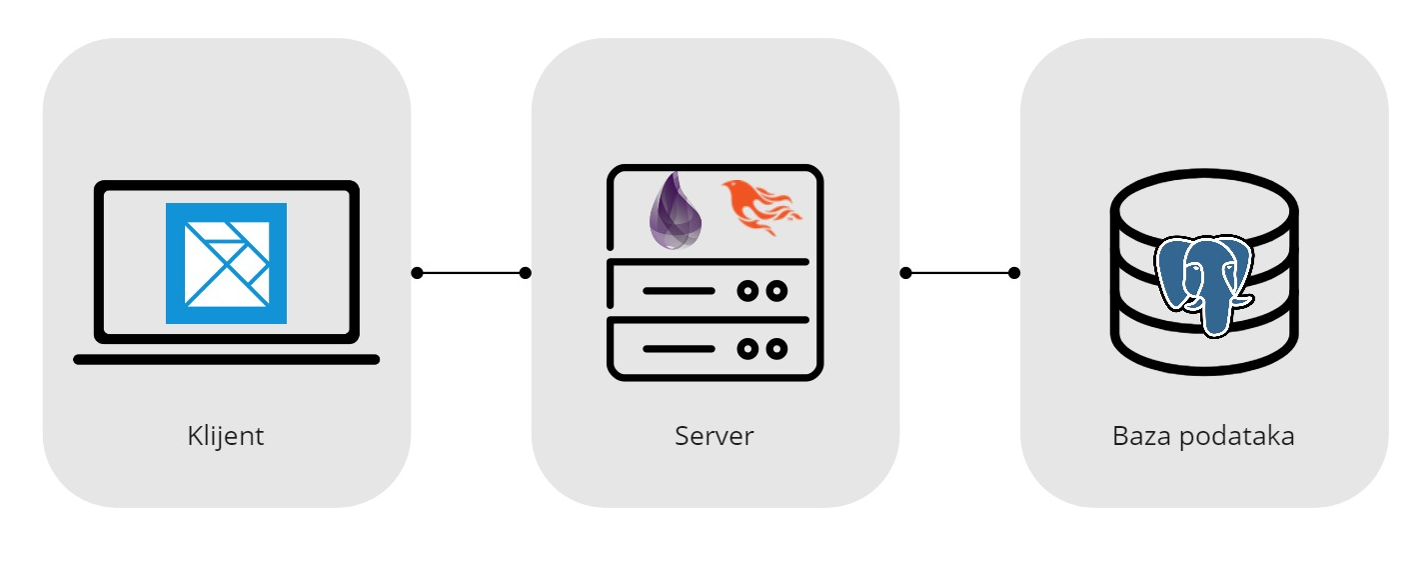
\includegraphics[width=0.9\textwidth]{msnr-arch.png}
  \caption{Arhitektura portala MSNR}
  \label{fig:msnr-arch}
\end{figure}

\section{Šema baze i opis osnovnih entiteta aplikacije}
Na slici \ref{fig:msnr-db} data je šema baze gde su prikazani osnovni entiteti i relacije između njih, u nastavku je dat njihov opis.
\begin{figure}[!ht]
  \centering
  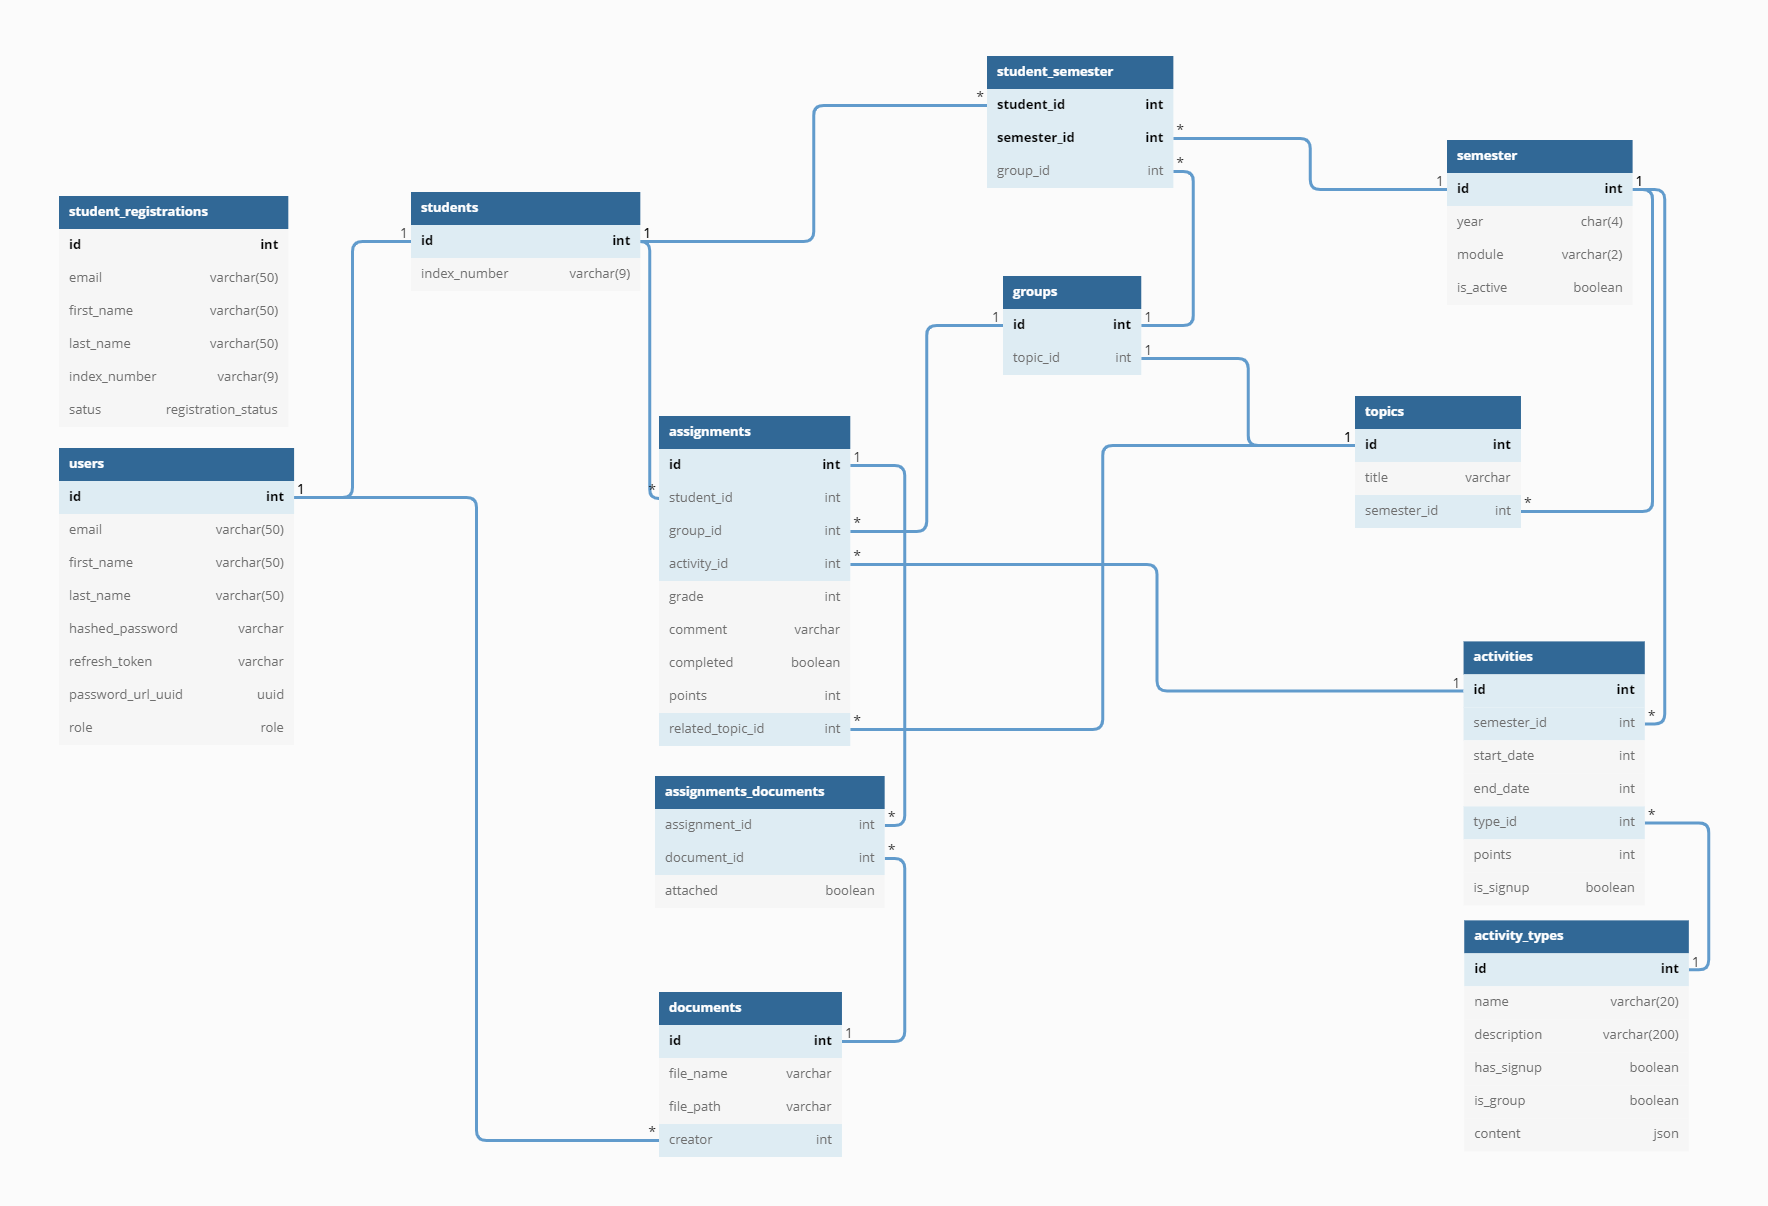
\includegraphics[width=0.95\textwidth]{msnr-db.png}
  \caption{Dijagram tabela portala MSNR}
  \label{fig:msnr-db}
\end{figure}

\paragraph{Zahtev za registraciju studenata}
Zahtev za registraciju, pored entiteta semestar i korisnik, predstavlja polazni entitet. Predstavljen je tabelom \emph{student{\textunderscore}registrations} i sadrži
informacije potrebne za registrovanje studenata --- ime, prezime, broj indeksa i email adresu, kao i status zahteva koji označava da li je odobren, odbijen ili nerazrešen.

\paragraph{Korisnik}
Tabela \emph{users} predviđena je za upravljanje korisničkim nalozima. Mogu postojati dva tipa, odnosno uloge, korisnika --- student i profesor. 
Pored osnovnih informacija o korisniku --- ime, prezime, rola i email, sadrži šifrovanu lozinku (\emph{hashed{\textunderscore}password}), osvežavajući
token (\emph{refresh{\textunderscore}token}) čija će upotreba biti objšnjena kasnije, i jedinstveni univerzalni identifikator koji se koristi prilikom postvaljanja lozinke
pre prvog prijavljivanja ili u slučaju da se zaboravi. Inicijalno će postojati profesorski nalog u tabeli, a prilikom prihvatanja zahteva za registraciju kreira se studentski nalog
i studentu se šalje mail sa vezom za postavljanje lozinke. 

\paragraph{Semestar}
Sve aktivnosti studenata vezane su za semestar, koji se predstavlja godinom u kojoj se održava i oznakom da li je aktivan, gde samo jedan semestar može biti trenutno aktivan. 

\paragraph{Student}
Kada profesor prihvati zahtev za registraciju, pored unosa u tabelu korisnici, vrše se još dva unosa --- jedan u tabelu \emph{students}, koja sadrži samo referencu ka korisniku i broj indeksa studenta, i 
drugi u tabelu koja predstavlja relaciju studenta i semestra --- \emph{students{\textunderscore}semestars}. Ova tabela, pored referenci ka studentu i semestru, ima i referencu ka grupi tako da 
svaki student u toku jednog semestra može biti član samo jedne grupe.

\paragraph{Grupa}
Prilikom prijave grupe, kreira se novi unos u tabeli grupe, dok se u tabeli \emph{students{\textunderscore}semestars} unosi
referenca ka kreiranoj grupi za sve studente iz grupe. Tabela grupe sadrži i referencu ka temi koja se unosi prilikom odabira teme.

\paragraph{Tema seminarskog rada} 
Profesor unosi naslove tema seminarskih radova koji se mogu odabrati u toku trenutnog semestra. Teme su predstavljene tabelom \emph{topics} i sadrže naslov, redni broj i referencu ka semestru u kom se mogu odabrati.

\paragraph{Aktivnost i tip aktivnosti}
Navedene aktivnosti na početku poglavlja su zapravo tipovi aktivnosti koji su predstavljeni tabelom \emph{activity{\textunderscore}types},
a aktivnosti (tabela \emph{activities}) predstavljaju relaciju između tipa aktivnosti i semestra. 
Tip aktivnosti sadrži naziv i opis aktivnosti, jedinstven k\^{o}d, oznake da li ima prijavu i da li je grupna aktivnost, i sam sadržaj aktivnosti.
Pored reference ka semestru i tipu, aktivnost sadrži informacije o periodu u kom se može izvršiti, broju poena koji nosi i oznaku da li predstavlja
samo prijavu za referisani tip ili konkretno izvršavanje.

\paragraph{Dodeljene aktivnosti}
Dodeljena aktivnost je centralni entitet portala i predstavljena je tabelom \emph{assignments}. U zavisnosti da li je aktivnost grupna ili ne, dodeljena aktivnost će imati referencu
ka studentu ili grupi. Neke aktivnosti, kao u slučaju recenzije, mogu se odnositi na određenu temu zbog čega je dodata kolona \emph{related{\textunderscore}topic{\textunderscore}id}. Pored
navedenih referenci, tabela sadrži i broj poena koji je osvojen, komentar koji je ostavio profesor, kao i oznaku da li je dodeljena aktivnost urađena. 

\paragraph{Dokument}
Veliki broj aktivnosti se zasniva na predaji dokumenata. Svi predati dokumenti nalaziće se na serveru, a u tabeli \emph{documents} čuvaće se informacije o nazivu, lokaciji dokumenta
na serveru i referenca ka korisniku koji je priložio dokument. Tabela \emph{assignments{\textunderscore}documents} označava koja dokumenta su povezana sa kojom dodeljenom aktivnosti, a
pored referenci ka ovim tabelama, sadrži i oznaku da li je taj dokument prikačen --- što označava da je taj dokument priložio profesor.

\chapter{Implementacija serverskog dela portala}

Programski jezik \emph{Elixir}, kao jezik opšte namene, nema ugrađenu podršku za razvoj
veb aplikacija i za tu svrhu razvojni okvir \emph{Phoenix} predstavlja najpopularniji izbor.
U prvod delu ove glave predstavljen je deo razvojnog okvira \emph{Phoenix} na primeru
portala MSNR, nakon čega je opisana implenentacija osnovnih delova samog portala.

\section{Razvojni okvir Phoenix}

Razvojni okvir \emph{Phoenix} napisan je na programskom jeziku \emph{Elixir} i razvija se uporedo
sa samim jezikom. Jedan od autora razojnog okvira je i Žozé Valim (autor jeziku \emph{Elixir}).
Analogno uticaju programskog jezika \emph{Ruby} na \emph{Elixir}, razvojni okvir \emph{Phoenix} je
u velikoj meri inspirisan razvojnim okvirom \emph{Ruby on Rails}, ali i drugim popularnim razvojnim okvirima.

\subsection{Instalacija razvojnog okvira}
Instaliranjem \emph{Elixir}-a ujedno je instaliran i osnovni alat za rad sa \emph{Elixir} projektima --- \emph{Mix}, koji se koristi za
kreiranje, kompajliranje i testiranje projekata, instaliranje i objavljivanje paketa, kao i za upravljanje zavisnim paketima projekta.
Upravo se pomoću njega instalira razvojni okvir \emph{Phoenix} i alat za generisanje \emph{Phoenix} projekata, ali prethodno je potrebno instalirati
\emph{Hex} \cite{hex} --- menadžer paketa za ekosistem \emph{Erlang}. Instalacija potrebnih alatki prikazana je u primeru koda \ref{listing:installPhxNew}.
Pored navedenih alatki potrebno je instalirati i \emph{PostgreSQL}.

\begin{listing}[h]
\begin{minted}{bash}
  mix local.hex
  mix archive.install hex phx_new
\end{minted}
\caption{Instalacija alatki \emph{hex} i \emph{phx{\textunderscore}new}}
\label{listing:installPhxNew}
\end{listing}

\subsection{Kreiranje i struktura projekta}
\emph{Phoenix} je okvir za razvoj svih tipova veb aplikcaija, omogućava iscrtavanje \emph{HTML}-a na serverskoj strani i ima odličnu podršku
za komunikaciju u realnom vremenu. Poseduje i svojstven koncept \emph{LiveView} koji pruža bogato korisničko iskustvo u realnom vremenu sa
iscrtavanjem na serverskoj strani. Za potrebe implementacije portala MSNR kreira se jednostavan veb API i prethodno navedene mogućnosti nisu potrebne.
Takođe, portal ne podržava lokalizaciju, stoga nema potreba za uključivanje modula \emph{gettext}.

Komanda korišćena za kreiranje projekta:
\mint{bash}|mix phx.new msnr_api --no-assets --no-html --no-gettext|
\noindent Parametrom \emph{-{}-no-assets} isključuje se generisanje direktorijuma \emph{assets} koji je predviđen za \emph{JavaScript} i \emph{CSS} datoteke,
dok se postavljanjem \emph{-{}-no-html} isključuje generisanje \emph{HTML} šablona za serversko iscrtavanje.
\begin{figure}[!h]
  \centering
  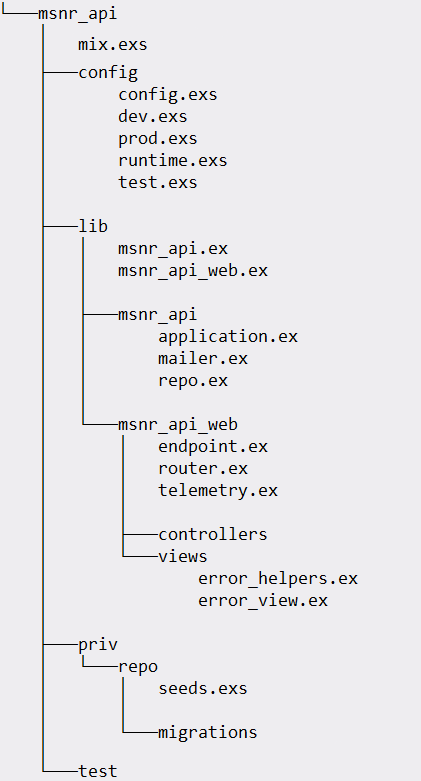
\includegraphics[width=0.5\textwidth]{msnr-dir.png}
  \caption{Struktura \emph{Phoenix} projekta}
  \label{fig:msnr-dir}
\end{figure}
Nakon uspešno izvršene komande, struktura projekta prikazana je na slici \ref{fig:msnr-dir}.

Nastali projekat je u osnovi \emph{Mix} projekat sa \emph{Phoenix} proširenjima. Svaki \emph{Mix} projekat ima
konfiguracionu datoteku \emph{mix.exs}, direktorijum \emph{lib} koji sadži osnovni k\^{o}d i direktorijum \emph{test} sa testovima.
Datoteka \emph{mix.exs} sadrži osnovne informacije o projektu --- kako se kompajlira, pokreće i 
listu zavisnih paketa koji se koriste u projektu. Nakon kompajliranja projekta, generisaće se datoteka \emph{mix.lock} koja
čuva precizne verzije zavisnih paketa čime se garantuje da se u produkciji koriste iste verzije kao i tokom razvoja.

Razvojni okvir \emph{Phoenix} dodaje i konfiguracije vezane za okruženje u kom se aplikacija izvršava. 
Podržana okruženja su razvojno (\emph{dev.exs}), testno (\emph{test.exs}) i produkciono (\emph{prod.exs}) i konfiguracije su smeštene u direktorijumu \emph{config},
zajedno sa glavnom konfiguracijom (\emph{config.exs}) koja se odnosi na sva okruženja. Mogu se dodati i druga ukoliko je potrebno, a pored navedenih
u direktorijumu \emph{config} nalazi se i \emph{runtime.exs} konfiguracija zadužena za učitavanje šifri (eng. \emph{secrets}) i drugih konfiguracionih vrednosti
iz varijabli okruženja.

U razvojnom okviru \emph{Phoenix} projekti se organizuju po kontekstima (eng. \emph{context}). Kontekst predstavlja modul koji grupiše funkcije sa
zajedničkom svrhom. Direktorijum \emph{lib} sadrži dva konteksta, odnosno modula: \emph{MsnrApi} koji enkapsulira svu domensku i
poslovnu logiku i modul \emph{MsnrApiWeb} koji definiše veb interfejs. Podmoduli se definišu u direktorijumima \emph{msnr{\textunderscore}api}
i \emph{msnr{\textunderscore}api{\textunderscore}web}. 
Kontekst \emph{MsnrApi} se odnosi na \emph{Model} u smislu arhitekture \emph{MVC --- Model-View-Controller} i u njemu će se definisati svi entiteta i
funkcije za rad sa njima. Inicijalno su kreirani:
\begin{itemize}
  \item \emph{MsnrApi.Application} --- modul zadužen za pokretanje aplikacije,
  \item \emph{MsnrApi.Repo} --- modul zadužen za komunikaciju sa bazom,
  \item \emph{MsnrApi.Mailer} --- modul zadužen za slanje elektronske pošte.
\end{itemize}
Kontekst \emph{MsnrApiWeb} sadrži implementaciju za poglede i upravljače unutar arhitekture \emph{MVC}.
Direktorijum \emph{controllers} je inicijalno prazan, dok su u direktorijumu \emph{views} kreirani pomoćni moduli za prikazivanje grešaka.
Moduli \emph{MsnrApiWeb.Endpoint} i \emph{MsnrApiWeb.Router} imaju ulogu da pripreme \emph{HTTP} zahtev i proslede ga odgovarajućem
upravljaču.

Direktorijum \emph{priv} sadrži sve resurse koji su potrebni u produkciji ali nisu direktan deo izvornog koda. U slučaju portala MSNR
sadržaće skripte vezane za menjanje i popunjavanje baze podataka. Testiranje, kao ni telemetrija, nije tema ovog rada.

\subsection{Obrada HTTP zahteva}

U osnovi obrade \emph{HTTP} zahteva nalazi se biblioteka \emph{Plug} \cite{plug}, koja se koristi gotovo kroz sve faze obrade zahteva.
Osnovne komponente razvojnog okvira \emph{Phoenix}, kao što su \emph{Endpoint}, ruter i upravljači, su interno utikači (eng. \emph{plug}).
Utikač predstavlja funkciju čija je ulazna i povratna vrednost \emph{Plug.Conn} struktura koja sadrži sve informacije o
primljenom \emph{HTTP} zahtevu. Veb server daje početne podatke za obradu zahteva, nakon čega \emph{Phoenix} poziva utikače jedan za drugim,
gde svaki utikač transformiše strukturu \emph{Plug.Conn} dok se obrada ne završi i odgovor pošalje korisniku. Za upotrebu utikača neophodan je
veb server i njegovo povezivanje sa utikačem, stoga je automatski ubačena zavisnost \texttt{\textbf{plug{\textunderscore}cowboy}} u \emph{mix.exs}
--- \emph{Cowboy} je najpopularniji veb server u ekosistemu \emph{Erlang}.

\begin{listing}[!ht]
\begin{minted}[fontsize=\footnotesize]{elixir}
defmodule MsnrApiWeb.Endpoint do
  use Phoenix.Endpoint, otp_app: :msnr_api

  plug Plug.Static, ...
  plug Plug.RequestId
  plug Plug.Telemetry, ...
  plug Plug.Parsers, ...
  plug Plug.MethodOverride
  plug Plug.Head
  plug Plug.Session, ...
  plug MsnrApiWeb.Router
end
\end{minted}
\caption{Utikači modula \emph{Endpoint}}
\label{listing:plugsEndpoint}
\end{listing}
Modul \emph{MsnrApiWeb.Endpoint} predstavlja početnu tačku prilikom obrade \emph{HTTP} zahteva i sastoji se od niza utikača. Kostur
modula prikazan je u primeru koda \ref{listing:plugsEndpoint}. Navedeni utikači imaju različite uloge --- za prikazivanje statičkih datoteka, za logovanje,
za parsiranje i druge. Svaki zahtev prolazi kroz sve navedene utikače. Postavljaju se pomoću makroa \texttt{\textbf{plug}}, a njihovo
navođenje se može posmatrati kao korišćenje operatora prosleđivanja, što je prikazano u primeru koda \ref{listing:plugsPipeline}.
\begin{listing}[!h]
\begin{minted}[fontsize=\footnotesize]{elixir}
connection
|> Plug.Static.call()
|> Plug.RequestId.call()
|> Plug.Telemetry.call()
|> Plug.Parsers.call()
|> Plug.MethodOverride.call()
|> Plug.Head.call()
|> Plug.Session.call()
|> MsnrApiWeb.Router.call()
\end{minted}
\caption{Prikaz pozivanja utikača pomoću operatora \texttt{\textbf{|>}}}
\label{listing:plugsPipeline}
\end{listing}

\subsubsection{Ruter}
Poslednji utikač modula \emph{Endpoint} je \emph{Router} koji se takođe sastoji od utikača, ali se oni grupišu
u tokove (eng. \emph{pipeline}). Unutar modula \emph{Router}, na osnovu putanje iz zahteva defnišu se opsezi
(eng. \emph{scope}), u kojima se navodi tok utikača koji će se koristiti i upravljači koji će se pozivati za određene rute.
Deo modula \emph{Router} koji sadrži definicije toka i opsega dat je u primeru koda \ref{listing:router}.
\begin{listing}[!h]
\begin{minted}[fontsize=\footnotesize]{elixir}
defmodule MsnrApiWeb.Router do
use MsnrApiWeb, :router

pipeline :api do
  plug :accepts, ["json"]
  plug MsnrApiWeb.Plugs.TokenAuthentication
end

scope "/api", MsnrApiWeb do
  pipe_through :api

  get "/auth/refresh", AuthController, :refresh
  post "/auth/login", AuthController, :login
  get "/auth/logout", AuthController, :logout

  resources "/activity-types", ActivityTypeController, except: [:new, :edit]
  ...
\end{minted}
\caption{Deo modula \emph{MsnrApiWeb.Router}}
\label{listing:router}
\end{listing}

U slučaju portala MSNR definisan je jedan tok i jedan opseg koji nadgleda sve zahteve koji počinju sa \emph{/api}.
Svaki od tih zahteva prolazi kroz prethodno definisani tok, nakon čega se na osnovu metoda \emph{HTTP} zahteva i nastavka
putanje poziva određena akcija, tj. funkcija iz navedenog upravljača. Na primer, za zahtev sa metodom
\emph{GET} i putanjom \emph{/api/auth/refresh} poziva se funkcija \emph{refresh} iz upravljača 
\emph{AuthController}. Za upravljač tipova aktivnosti koristi se funkcija \emph{resource} koja
predstavlja skraćenu sintaksu za navođenje ruta. Jednim pozivom se kreira mapiranje metoda za akcije
(\texttt{\textbf{index}}, \texttt{\textbf{new}}, \texttt{\textbf{create}}, \texttt{\textbf{show}}, \texttt{\textbf{edit}},
\texttt{\textbf{update}}, i \texttt{\textbf{delete}}) koje su komplementarne REST akcijama. Poslednji argument označava da
će se izostaviti akcije \texttt{\textbf{new}} i \texttt{\textbf{edit}} koje se koriste prilikom upotrebe \emph{HTML} šablona. Takođe je moguće
navesti i samo akcije koje će se koristiti pomoći atoma \texttt{\textbf{:only}} umesto \texttt{\textbf{:except}}. U primeru koda \ref{listing:routes}
prikazan je deo rezultata izvršene komande \texttt{\textbf{mix phx.routes}} koja izlistava sve definisane rute aplikacije i njihovo mapiranje na upravljače.
\begin{listing}[!h]
  \begin{minted}[fontsize=\scriptsize]{bash}
$ mix phx.routes
         auth_path  GET     /api/auth/refresh        AuthController :refresh
         auth_path  POST    /api/auth/login          AuthController :login
         auth_path  GET     /api/auth/logout         AuthController :logout
activity_type_path  GET     /api/activity-types      ActivityTypeController :index
activity_type_path  GET     /api/activity-types/:id  ActivityTypeController :show
activity_type_path  POST    /api/activity-types      ActivityTypeController :create
activity_type_path  PATCH   /api/activity-types/:id  ActivityTypeController :update
                    PUT     /api/activity-types/:id  ActivityTypeController :update
activity_type_path  DELETE  /api/activity-types/:id  ActivityTypeController :delete
...
\end{minted}
\caption{Izlistavanje ruta komandom \texttt{\textbf{mix phx.routes}}}
\label{listing:routes}
\end{listing}

\subsubsection{Upravljači i pogledi}
Budući da je upravljač takođe utikač, njegova osnovna uloga je da sakupi i pripremi podatke za sledeći korak obrade korisničkog zahteva.
To može uključiti pozivanje baze podataka, eksternog veb servisa ili obradu neke statičke datoteke. 
Na primeru upravljača \emph{ActivityTypeController} u primeru koda \ref{listing:controller} može se videti generalna struktura upravljača
i implementacija akcije \texttt{\textbf{:index}}.
\begin{listing}[!h]
\begin{minted}[fontsize=\footnotesize]{elixir}
defmodule MsnrApiWeb.ActivityTypeController do
  use MsnrApiWeb, :controller

  alias MsnrApi.ActivityTypes

  def index(conn, _params) do
    activity_types = ActivityTypes.list_activity_types()
    render(conn, "index.json", activity_types: activity_types)
  end

  def create(conn, %{"activity_type" => activity_type_params}) do
    ...
  end

  def show(conn, %{"id" => id}) do
    ...
  end

  def update(conn, %{"id" => id, "activity_type" => activity_type_params}) do
    ...
  end

  def delete(conn, %{"id" => id}) do
    ...
  end
end
\end{minted}
\caption{Primer strukture upravljača}
\label{listing:controller}
\end{listing}

Poslednji poziv u akciji upravljača je funkcija \texttt{\textbf{render}} definisana u modulu \emph{ActivityTypeView} koja za argumente ima \emph{Plug.Conn} strukturu,
naziv šablona i podatke potrebne za iscrtavanje. U slučaju \emph{JSON} veb interfejsa kreira se mapa koja se prevodi u \emph{JSON} objekat,
čime se završava obrada zahteva unutar razvojnog okvira \emph{Phoenix}. 

\subsection{Komunikacija sa bazom podataka}
Za komunikaciju sa bazom podataka u \emph{Elixir} projektima pretežno se koristi biblioteka \emph{Ecto} \cite{ecto}.
Ona nije sastavni deo razvojnog okvira \emph{Phoenix}, ali se podrazumevano uključuje i prilikom kreiranja
\emph{Phoenix} projekta u se potrebni \emph{Ecto} moduli i konfiguracija. Ukoliko nije potrebno
korišćenje ove biblioteke prilikom kreiranja projekta navodi se parametar \emph{-{}-no-ecto}.

Biblioteka \emph{Ecto} pruža jednostavan način za izvršavanje upita, transakcija, opisivanje kako se strukture mapiraju
u odrđene tabele i navođenje odnosa modula. Ima specifičan koncept pod nazivom \emph{skup promena} (eng. \emph{changeset}) koji enkapsulira ceo
proces prihvatanja eksternih podataka, validiranja, konvertovanja i proveravanja dodatnjih uslova pre nego što se upišu u bazu. Osnovni moduli biblioteke su:
\begin{itemize}
  \item \emph{Ecto.Repo} --- za definisanje omotača oko baze podataka preko kog se ostvaruje komunikacija sa bazom, opisuje gde se nalaze podaci,
  \item \emph{Ecto.Schema} --- za definisanje mapiranja eksternih podataka u \emph{Elixir} strukture, opisuje šta su podaci,
  \item \emph{Ecto.Query} --- za definisanje upita u \emph{Elixir} sintaksi, opisuje kako se čitaju podaci,
  \item \emph{Ecto.Changeset} --- za praćenje i validiranje izmena, opisuje kako se menjaju podaci.
\end{itemize}
Za integraciju sa bibliotekom \emph{Ecto}, \emph{Phoenix} uključuje paket \texttt{\textbf{phoenix{\textunderscore}ecto}},
adapter za bazu podataka \emph{PostgreSQL} ---\texttt{\textbf{postgrex}} i paket \texttt{\textbf{ecto{\textunderscore}sql}}
koji pored prethodno navedenih \emph{Ecto} osobina ima i podršku za migracije, što omogućava menjanje i praćenje strukture
baze tokom vremena.
\begin{listing}[!h]
  \begin{minted}{elixir}
  config :msnr_api,
    ecto_repos: [MsnrApi.Repo]
\end{minted}
\caption{Navođenje \emph{Ecto} repozitorijuma u konfiguraciji}
\label{listing:configRepo}
\end{listing}
U generisanom modulu \emph{MsnrApi.Repo} definiše se repozitorijum i adapter koji se koristi. Repozitorijum koji se koristi neophodno je navesti u
glavnoj konfiguraciji \emph{config.exs}, što je prikazano u primeru koda \ref{listing:configRepo}. \emph{Ecto} podržava rad sa više repozitorijuma istovremeno, 
zato se navodi lista naziva repozitorijuma. Parametri za definisanje komunikacije sa bazom podataka postavljaju se posebno za svako okruženje.
U primeru koda \ref{listing:dbDevConfig} prikazana je konfiguracija za razvojno okruženje (\emph{config/dev.exs}) i pokretanjem komande
\texttt{\textbf{mix ecto.create}} lokalno se kreira \texttt{\textbf{msnr{\textunderscore}api{\textunderscore}dev}} baza podataka. 
\begin{listing}[!h]
  \begin{minted}{elixir}
    config :msnr_api, MsnrApi.Repo,
    username: "postgres",
    password: "postgres",
    database: "msnr_api_dev",
    hostname: "localhost",
    show_sensitive_data_on_connection_error: true,
    pool_size: 10
\end{minted}
\caption{Konfiguracija baze podataka u razvojnom okruženju}
\label{listing:dbDevConfig}
\end{listing}

\subsubsection{Definisanje entiteta}
Budući da kontekst \emph{MsnrApi} sadži domensku logiku aplikacije, u njemu su definisani svi entiteti aplikacije, takođe
kao konteksti. Na primeru tipa aktivnosti, pod direktorijumom \emph{msnr{\textunderscore}api} nalazi se direktorijum
\emph{activity{\textunderscore}types} sa definicijom strukture \emph{ActivityType} kojom se predstavlja
entitet i datoteka \emph{activity{\textunderscore}types.ex} u kojoj je definisan modul \emph{ActivityTypes} sa
funkcijama za rad sa entitetom.

\emph{Ecto} omogućava definisanje struktura čija se pojedinačna polja povezuju sa kolonama u bazi podataka. 
U primeru koda \ref{listing:activityType} prikazano je definisanje entiteta tipa aktivnosti korišćenjem modula
\emph{Ecto.Schema}.
\begin{listing}[!h]
  \begin{minted}[fontsize=\footnotesize]{elixir}
    use Ecto.Schema
    import Ecto.Changeset
  
    schema "activity_types" do
      field :content, :map
      field :description, :string
      field :has_signup, :boolean, default: false
      field :is_group, :boolean, default: false
      field :name, :string
      field :code, :string
  
      has_many :activities, MsnrApi.Activities.Activity
  
      timestamps()
    end
  ...
\end{minted}
\caption{Upotreba \emph{Ecto.Schema} na primeru tipa aktivnosti }
\label{listing:activityType}
\end{listing}
Makroi \texttt{\textbf{schema}} i \texttt{\textbf{filed}} definišu istovremeno tabelu u bazi i Elixir
strukturu. Svako polje definisano makroom \texttt{\textbf{filed}} odgovara polju u strukturi 
\emph{ActivityType} i polju, odnosno koloni, tabele \emph{activity{\textunderscore}types}.
Makro \texttt{\textbf{filed}} ima tri argumenta --- naziv polja, tip i opcije. U prikazanom primeru korišćena je
opcija za postavljanje podrazumevane vrednosi kolone. Funkcija \texttt{\textbf{timestamps}} dodaje još dva polja,
\texttt{\textbf{created{\textunderscore}at}} i \texttt{\textbf{inserted{\textunderscore}at}} za praćenje 
promena entiteta u bazi. 

Makroom \texttt{\textbf{has{\textunderscore}many}} opisuje se asocijacija 
entiteta --- jedan tip aktivnosti se može navesti u više aktivnosti. Sa druge strane, svaka aktivnost ima svoj tip,
tako da se u modulu \emph{MsnrApi.Activities.Activity} asocijacija sa odgovarajućim tipom aktivnosti definiše pomoću \texttt{\textbf{belongs{\textunderscore}to}}.
Pored navedenih, za druge tipove asocijacija
mogu se koristiti makroi \texttt{\textbf{has{\textunderscore}one}} i \texttt{\textbf{many{\textunderscore}many}}.

Pored prikazanih polja, \emph{Ecto} podrazumevano dodaje i \texttt{\textbf{:id}} polje
koje predstavlja primarni ključ tabele. U sličaju kada je potrebno drugačije definisati primarni ključ koristi
se atribut \texttt{\textbf{@primary{\textunderscore}key}}, što se može videti na primeru definisanja studenta.

\subsubsection{Migracije}
Kreiranjem šeme entiteta, definiše se način na koji \emph{Ecto} komunicira sa bazom, dok se kreiranje odgovarajućih
tabela u bazi vrši migracijama. Migracije su predstavljane modulima u kojima se definišu promene koje će se izvršiti nad
bazom i pružaju mogućnost da se izvršene promene ponište. Kreiraju se pomoću \emph{Mix} komande 
\texttt{\textbf{mix ecto.gen.migration \emph{<naziv migracije>}}} i nalaze se u direktorijumu
\emph{priv/repo/migrations}, a naziv datoteke je oblika \emph{<vreme kreiranja>{\textunderscore}<naziv migracije>.exs}.
U primeru koda \ref{listing:activityTypeMigration} prikazana je migracija kojom se kreira tabela \emph{activity{\textunderscore}types} i
dodaju jedinstveni indeksi za naziv i k\^{o}d tipa aktivnosti.
\begin{listing}[!h]
  \begin{minted}[fontsize=\footnotesize]{elixir}
    defmodule MsnrApi.Repo.Migrations.CreateActivityTypes do
    use Ecto.Migration
  
    def change do
      create table(:activity_types) do
        add :name, :string, null: false
        add :code, :string, null: false
        add :description, :string, null: false
        add :has_signup, :boolean, default: false, null: false
        add :is_group, :boolean, default: false, null: false
        add :content, :map
  
        timestamps()
      end
  
      create unique_index(:activity_types, [:name])
      create unique_index(:activity_types, [:code])
    end
  end
\end{minted}
\caption{Migracija za kreiranje tabele \emph{activity{\textunderscore}types}}
\label{listing:activityTypeMigration}
\end{listing}

Migracije se mogu definisati na dva načina --- prvi, predstavljen u primeru koda, koristi funkciju \texttt{\textbf{change}}
i drugi sa dve funkcije \texttt{\textbf{up}} i \texttt{\textbf{down}}, kojima se difinišu akcije koje prilikom izvršavanja i
poništavanja migracije. U slučaju funkcije \texttt{\textbf{change}} \emph{Ecto} sam zaključuje potrebne korake prilikom
poništavanja migracije. Prilikom implementacije portala MSNR funkcije \texttt{\textbf{up}} i \texttt{\textbf{down}} korišćene
su za definisanje tipova uloga korsnika i statusa registracije.

\subsubsection{Kreiranje, preuzimanje i brisanje podataka iz baze}
\emph{Ecto} pruža brojne funkcije za interakciju sa bazom podataka kroz modul \emph{Ecto.Repo}.
U tabeli \ref{table:repoFuntions} prikazane su najčešće korišćene funkcije i njihov kratak opis.
\begin{table}[h!]
  \renewcommand*{\arraystretch}{1.4}
  \small
  \centering
  \begin{tabular}{p{0.1\textwidth} | p{0.39\textwidth} | p{0.42\textwidth}}
    Funkcija & Opis & Povratna vrednost\\ [0.5ex] 
    \hline
    \texttt{all} & Vraća svaki red iz tabele za zadati upit & Lista redova \\ 
    \texttt{get} & Vraća jedan red za zadati primarni ključ & Red ili \texttt{nill} ako nije pronađen  \\
    \texttt{one} & Vraća jedan red za zadati upit &  Red ili \texttt{nill} ako nije pronađen, ukoliko pronađe više redova izbacuje izuzetak \\
    \hline
    \texttt{delete} & Briše red iz tabele na osnovu primarnog ključa iz struktue & \texttt{\{:ok, red\}} \\ 
    \texttt{insert} & Dodaje red u tabeli na osnovu date strukture & \texttt{\{:ok, red\}} ili \texttt{\{:error, changeset\}}\\
    \texttt{update} & Ažurira red u tabeli na osnovu date strukture sa primarnim ključem & \texttt{\{:ok, red\}} ili \texttt{\{:error, changeset\}} \\
  \end{tabular}
  \caption{Funkcije modula \emph{Ecto.Repo} za rad sa bazom podataka}
  \label{table:repoFuntions}
  \end{table}

Funkcije \texttt{get} i \texttt{one} imaju verzije sa znakom \texttt{\textbf{!}}
na kraju naziva (npr. \texttt{get!}) koje u slučaju da red nije pronađen izbacuju izuzetak.
U slučaju funkcija za modifikaciju podataka, takođe postoje pandan funkcije sa \texttt{\textbf{!}} u nazivu
i prilikom greške izbacuju izuzetak. One prilikom uspešnog izvršavanja vraćaju samo red, bez torke.

U primeru koda \ref{listing:ActivityTypes} prikazan je modul
\emph{MsnrApi.ActivityTypes} i način upotrebe nekih od funkcija iz tabele. Za izlistavanje tipova aktivnosti,
funkciji \texttt{all} se prosleđuje samo naziv tabela, tako da funkcija vraća sve redove.
\begin{listing}[!h]
  \begin{minted}[fontsize=\footnotesize]{elixir}
    defmodule MsnrApi.ActivityTypes do
    alias MsnrApi.Repo
  
    alias MsnrApi.ActivityTypes.ActivityType
  
    def list_activity_types do
      Repo.all(ActivityType)
    end
  
    def get_activity_type!(id), do: Repo.get!(ActivityType, id)
  
    def create_activity_type(attrs \\ %{}) do
      %ActivityType{}
      |> ActivityType.changeset(attrs)
      |> Repo.insert()
    end
  
    def update_activity_type(%ActivityType{} = activity_type, attrs) do
      activity_type
      |> ActivityType.changeset(attrs)
      |> Repo.update()
    end
  
    def delete_activity_type(%ActivityType{} = activity_type) do
      Repo.delete(activity_type)
    end
  end
\end{minted}
\caption{Definica modula \emph{MsnrApi.ActivityTypes}}
\label{listing:ActivityTypes}
\end{listing}

\subsubsection{Definisanje upita}
Modul \emph{Ecto.Query} pruža sintaksu za pisanje upita koja je veoma slična samoj \emph{SQL} sintaksi. 
S tim da sintaksa upita započinje makroom \texttt{from} nakon čega se ostali delovi upita definišu pomoću liste ključnih reči.
Praksa je da se ključna reč \texttt{:select} navodi na kraju, kao kod \emph{LINQ} \cite{linq} sintakse iz razvojnog okvira \emph{.NET}
koja je bila inspiracija za \emph{Ecto}, a može se i izostaviti. Za interpolaciju parametara koristi se operator \texttt{ \^{}}.
Primer jednostavnog upita dat je u primeru koda \ref{listing:query-example} gde je prikazana funkcija za prikazivanje studentskih
registracija iz modula \emph{StudentRegistrations}.
\begin{listing}[h]
  \begin{minted}[fontsize=\footnotesize]{elixir}
    import Ecto.Query

    def list_student_registrations(semester_id) do
      Repo.all(
        from sr in StudentRegistration, where: sr.semester_id == ^semester_id)
    end
  \end{minted}
\caption{Primer upita definisanog pomoću modula \emph{Ecto.Query}}
\label{listing:query-example}
\end{listing}

Modul \emph{Ecto.Query} pruža mogućnost definisanja dinamičnih upita, podupita i dosta drugih karakteristika o kojima se može videti više na zvaničnoj stranici.

\subsubsection{Izmena entiteta}
U primeru koda \ref{listing:ActivityTypes} tokom kreiranja i izmene tipa aktivnosti poziva se
funkcija \emph{ActivityType.changeset} kojom se kreira skup promena. Prilikom kreiranja
podataka se može koristiti i struktura definisana sa \emph{Ecto.Schema}, dok je 
menjanje podataka moguće samo korišćenjem strukture \emph{Ecto.Changeset}.
Kreiranje strukture \emph{Ecto.Changeset} funkcijom \texttt{changeset} 
prikazano je u primeru koda \ref{listing:changeset}. 
\begin{listing}[!h]
\begin{minted}[fontsize=\footnotesize]{elixir}
    def changeset(activity_type, attrs) do
      activity_type
      |> cast(attrs, [:code, :name, :description, :has_signup, :is_group, :content])
      |> validate_required([:code, :name, :description, :content])
      |> unique_constraint(:name)
      |> unique_constraint(:code)
    end
\end{minted}
\caption{Definicija funkcije \texttt{changeset}}
\label{listing:changeset}
\end{listing}

Funkcija \texttt{cast} je pretežno prva u nizu funkcija koje se pozivaju i ograničava polja koja se mogu promeniti.
U prikazanom primeru, ne mogu se izmeniti polja \texttt{:id}, \texttt{:created{\textunderscore}at} i
\texttt{:inserted{\textunderscore}at}. Polje \texttt{:inserted{\textunderscore}at} će izmeniti sam \emph{Ecto}
prilikom izvršavanja funkcije \texttt{update}.

Zatim se funkcijama \texttt{validate{\textunderscore}required} i \texttt{unique{\textunderscore}constraint} 
proveravaju obavezna polja i jedinstvenost naziva i koda. Rezultat izvršavanja niza funkcija nad strukturom
\emph{Ecto.Changeset} je takođe struktura \emph{Ecto.Changeset}. Rezultujuća struktura sadrži mnoge informacije
među kojima su promene koje treba izvršiti, validnost izmena i greške validacije ukoliko ih ima.
Modul \emph{Ecto.Changeset} pruža brojne funkcije za validiranje, a moguće je definisati i prilagođene funkcije.

\subsubsection{Generisanje datoteka}
Prilikom definisanja entiteta, dodaje se njegov kontekst sa \emph{Ecto.Schema} strukturom, kao i migracija. 
Ukoliko je potrebno dodati i upravljač, to su još dve datoteke --- upravljač i pogled. Da bi se olakšao ovaj
proces, \emph{Phoenix} pruža komande za automatsko generisanje navedenih datoteka zajedno sa šablonima za testove.
Za potrebe portala MSNR najčešće korišćena komanda jeste \texttt{mix phx.gen.json} koja generiše sve prethodno
navedene datoteke. Prethodno prikazani listinzi vezani za \emph{ActivityType} entitet rezultat su komande prikazane u
primeru koda \ref{listing:gen-json}. Parametri su redom: naziv konteksta, naziv strukture i naziv tabele u bazi, nakon čega slede
definicije polja, odnosno kolona.
\begin{listing}[h]
  \begin{minted}[fontsize=\footnotesize,breaklines=true]{bash}
    mix phx.gen.json ActivityTypes ActivityType activity_types code:string:unique name:string:unique description:string has_signup:boolean is_group:boolean content:map
  \end{minted}
\caption{Upotreba \texttt{mix phx.gen.json} komande na primeru \emph{ActivityType} entiteta}
\label{listing:gen-json}
\end{listing}
Razvojno oktuženje \emph{Phoenix} pruža veliki broj komandi za generisanje, kao što su \texttt{mix phx.gen.context}, 
\texttt{mix phx.gen.shema} i mnoge druge, sa mnogim dodatnim opcijama, o čemu se može pročitati više na zvaničnoj dokumentaciji.

\section{Registrovanje studenata}
Registrovanje studenata može se podeliti u tri celine. Prva se odnosi na podnošenje, druga na prihvatanje
zahteva i kreiranje korisničkog naloga, a treća na završno podešavanje naloga --- postavljanje lozinke.

Prve dve celine se izvršavaju unutar upravljača \emph{StudentRegistrationController} čije su
osnovne akcije \texttt{create} za podnošenje zahteva, \texttt{index} za izlistavanje svih zahteva u toku
trenutnog semestra i \texttt{update} za obradu zahteva. Akcija za izlistavanje zahteva se razlikuje od drugih
po tome što uključuje i informaciju o semestru, tako da se za akciju \texttt{index} definiše putanja pod upravljačem
\emph{SemesterController}. Ovo je moguće zato što razvojni okvir \emph{Phoenix} omogućava definisanje potputanja, kao i korišćenje jednog upravljača u više putanja.
Putanje koje se koriste prilikom registrovanja studenata prikazane su u primeru koda \ref{listing:registration-routes}.
U poslednjem koraku registrovanja studenata koristi se upravljač \emph{PasswordController}.
\begin{listing}[h]
\begin{minted}[fontsize=\scriptsize]{elixir}
resources "/passwords", PasswordController, only: [:update]
resources "/registrations", StudentRegistrationController, except: [:new, :edit, :index]

resources "/semesters", SemesterController, except: [:new, :edit] do
  resources "/registrations", StudentRegistrationController, only: [:index]
... 
\end{minted}
\caption{Definisanje putanje za registrovanje studenata}
\label{listing:registration-routes}
\end{listing}

Unutar portala MSNR putanje su organizovane hijerarhijski, budući da se sve aktivnosti vrše u toku semestra,
putanja \emph{/semesters} se nalazi na vrhu hijerarhije. Delom koda prikazanim u prethodnom primeru koda registruju
se putanje \emph{api/semesters} za rad sa semestrima i \emph{api/semesters/<semester{\textunderscore}id>/registrations}
za izlistavanje registracija. Vrednost <semester{\textunderscore}id> iz putanje prosleđuje se kao parametar akciji
upravljača što je prikazano u primeru koda \ref{listing:index-registrations}.
\begin{listing}[h]
  \begin{minted}[fontsize=\scriptsize]{elixir}
    def index(conn, %{"semester_id" => semester_id}) do
      student_registrations = StudentRegistrations.list_student_registrations(semester_id)
      render(conn, "index.json", student_registrations: student_registrations)
    end
  \end{minted}
\caption{Definicija akcije \texttt{index} u upravljaču \emph{StudentRegistrationController}}
\label{listing:index-registrations}
\end{listing}

Podnošenje zahteva se izvršava slanjem \emph{POST} \emph{HTTP} zahteva za čiju obradu je dovoljan k\^{o}d generisan komandom
\texttt{mix phx.gen.json}, s tim da je prilikom kreiranja potrebno povezati zahtev sa aktivnim semestrom.
Sa druge strane, obrada zahteva od strane profesora unutar akcije \texttt{update} je dosta kompleksnija.
Unutar transakcije je potrebno ažurirati zahtev, kreirati nalog za studenta, ukoliko je prihvaćen, i poslati mail.
Funkcija za prihvatanje zahteva unutar modula \emph{StudentsRegistrations} prikazana je u primeru koda \ref{listing:accept-registration}.
\begin{listing}[h]
\begin{minted}[fontsize=\footnotesize]{elixir}
  def update_student_registration(
      %StudentRegistration{} = registration,
      %{"status" => "accepted"} = attrs
    ) do
    create_user = fn _repo, %{student_registration: reg} ->
      Accounts.create_student_account(reg)
    end

    create_student = fn _repo, %{user: user} ->
      Students.create_student(user, %{index_number: registration.index_number})
    end

    send_email = fn _repo, %{user: user} ->
      Emails.accept(user) |> Mailer.deliver()
    end

    Multi.new()
    |> Multi.update(
        :student_registration,
        StudentRegistration.changeset(registration, attrs))
    |> Multi.run(:user, create_user)
    |> Multi.run(:student, create_student)
    |> Multi.run(:email, send_email)
    |> MsnrApi.Repo.transaction()
  end
\end{minted}
\caption{Prihvatanje zahteva za registraciju studenta}
\label{listing:accept-registration}
\end{listing}
Sturktura \emph{Ecto.Multi} se koristiti za grupisanje više operacija nad repozitorijumom, pri čemu se svakoj
operaciji daje jedinstveno ime koja će identifikovati njen rezultat u slučaju uspeha ili neuspeha. Svaka od 
operacija mora vraćati rezultat oblika \texttt{\{:ok, vrednost\}} ili \texttt{\{:error, greška\}}.

Za slanje mejlova koristi se biblioteka \emph{Swoosh}, koja je, kao i \emph{Ecto}, uključena prilikom kreiranja
projekta. Modul \emph{MsnrApi.Mailer}, definisan slično kao i \emph{MsnrApi.Repo}, sadrži funkcije za slanje mailova.
Unutra modula \emph{MsnrApi.Emails} definišu se funkcije kojima se kreira sastav mejlova pomoću modula \emph{Swoosh.Email}.

Da bi student mogao da se prijavi na portal, potrebno je da postavi lozinku, čime se zaokružuje proces registracije.
U primeru koda \ref{listing:password-controller} prikazan je upravljač \emph{PasswordController} sa akcijom \texttt{update} koja je
zadužena za postavljanje lozinke. Parametri \texttt{email} i \texttt{password} dolaze iz tela zahteva, a \texttt{id} iz putanje
i očekuje se da odgovara vrednosti kolone \emph{pasword{\textunderscore}url{\textunderscore}path} iz tabele \emph{users}.

Nakon uspešne verifikacije korisnika, unutar funkcije \texttt{set{\textunderscore}password} poziva se
\texttt{User.password{\textunderscore}changeset} kojom se proverava dužina lozinke i vrši kriptovanje lozinke.
Ukoliko i provera lozinke prođe uspešno, šalje se odgovor sa statusom 200 bez sadržaja.

\begin{listing}[h!]
\begin{minted}[fontsize=\footnotesize]{elixir}
defmodule MsnrApiWeb.PasswordController do
use MsnrApiWeb, :controller
  
alias MsnrApi.Accounts
  
action_fallback MsnrApiWeb.FallbackController
  
def update(conn, %{"id" => uuid, "email" => email, "password" => password}) do
    with {:ok, user} <- Accounts.verify_user(%{email: email, uuid: uuid}),
         {:ok, _} <- Accounts.set_password(user, password) do
         send_resp(conn, :no_content, "")
      end
    end
end
\end{minted}
\caption{Definicija upravljača \emph{MsnrApiWeb.PasswordController}}
\label{listing:password-controller}
\end{listing}

Unutar svakog upravljača makroom \texttt{action{\textunderscore}fallback} se registruje utikač, odnosno upravljač,
\emph{MsnrApiWeb.FallbackController} koji se poziva u slučaju da dođe do greške prilikom izvršavanja akcije.
U slučaju da korisnik nije verifikovan, funkcija \texttt{verify{\textunderscore}user} vraća \texttt{\{:error, :unauthorized\}}
i pošto u \texttt{with} izrazu taj slučaj nije obrađen dolazi do greške. Greška se ne prosleđuje odmah korisniku već
se pomoću upravljača \emph{FallbackController} prevodi u 401 grešku i korisniku vraća validan odgovor. 

\section{Autentifikacija i autorizacija korisnika}
Autentifikacija i autorizacija korisnika portala MSNR zasnovana je na tokenima. Nakon uspešnog prijavljivanja korisniku
se prosleđuje token koji se prilikom svakog \emph{HTTP} zahteva šalje serveru kroz zaglavlje \emph{Authorization}.
Token nosi informacije o korisniku i ima ograničeno vreme trajanja, nakon čega više nije validan.
Pomoću utikača se prilikom obrade zahteva validira token i proveravaju prava pristupa određenim resursima.

Unutar implementacije portala MSNR koriste se dva tokena: \begin{itemize}
\item \emph{acceess{\textunderscore}token} --- Sadrži informacije o korisniku i koristi se za pristupanje portalu. Ima kraće vreme trajanja (do pola sata) i korsniku se prosleđuje kroz telo \emph{HTTP} odgovora.
\item \emph{refresh{\textunderscore}token} --- Koristi se za obnavljanje \emph{acceess{\textunderscore}token}, ima duže vreme trajanja (nekoliko dana) i prosležuje se u \emph{HttpOnly} i \emph{Secure} kolačiću.  
\end{itemize}

Prijavljivanje korisnika izvršava se unutar akcije \texttt{login} upravljača \emph{AuthController} i
način obrade zahteva je sličan akciji \texttt{refresh} za obnavljanje tokena. U prvoj se
korisnik verifikuje na osnovu imejla i lozinke, a u drugoj na osnovu sadržaja kolačića, nakon čega se kreiraju novi tokeni.
Razvojni okvir \emph{Phoenix} ima ugrađenu podršku za rad sa tokenima i preko modula \emph{Phoenix.Token}
pruža funkcije za potpisivanje i verifikaciju tokena koje se koriste unutar modula \emph{MsnrApiWeb.Authentication}.
Akcijom \texttt{logout} se uklanja token za obnavljanje iz kolačića i kada token za pristup istekne potrebno je ponovno prijavljivanje. 

\subsection{Utikač za autentifikaciju korisnika}
Uključivanje utikača \emph{MsnrApiWeb.Plugs.TokenAuthentication} prikazano je zajedno sa registrovanjem akcija upravljača
\emph{AuthController} u primeru koda \ref{listing:router} u poglavlju 5.3 prilikom opisa obrade \emph{HTTP} zahteva.
\begin{listing}[h!]
\begin{minted}[fontsize=\footnotesize]{elixir}
defmodule MsnrApiWeb.Plugs.TokenAuthentication do
import Plug.Conn

def init(opts), do: opts

def call(conn, _opts) do
  with ["Bearer " <> token] <- get_req_header(conn, "authorization"),
       {:ok, payload} <- MsnrApiWeb.Authentication.verify_access_token(token) do
    assign(conn, :user_info, payload)
  else
    _ ->
      assign(conn, :user_info, nil)
  end
end
end
\end{minted}
\caption{Definicija utikača \emph{MsnrApiWeb.Plugs.TokenAuthentication}}
\label{listing:authentication-plug}
\end{listing}
Njegova uloga jeste da, ukoliko se token verifikuje, informacije o korisniku iz tokena dodele trenutnoj konekciji tako
da se one mogu koristiti dalje u upravljačima. Definicija utikača \emph{MsnrApiWeb.Plugs.TokenAuthentication} prikazana je u
primeru koda \ref{listing:authentication-plug}.

\subsection{Utikač za autorizaciju studenata}
Utikači se mogu definisati na dva načina. Prvi, pomoću modula, prikazan je na primeru utikača za autentifikaciju,
i drugi, pomoću funkcije, kojim su definisani utikači za autorizaciju. Autorizacija pomoću utikača se zasniva na
proveri uloge korisnika i uključuju se različito za svaki upravljač.
Unutar modula \emph{MsnrApiWeb.Plugs.Authorization}
definisane su funkcije \texttt{professor{\textunderscore}only} i \texttt{allow{\textunderscore}students} koje imaju
iste argumente kao i funkcija \texttt{call} (primer koda \ref{listing:authentication-plug}) u slučaju modula.
Prilikom provere studentske uloge proverava se, ukoliko postoji, i \emph{student{\textunderscore}id} parametar iz putanje.
Upotreba utkača se može ograničiti na određene akcije unutar upravljača, što se može videti na primeru upravljača \emph{AssignmentController} (primer koda \ref{listing:authorization-plug}).
\begin{listing}[h!]
\begin{minted}[fontsize=\footnotesize]{elixir}
defmodule MsnrApiWeb.AssignmentController do
  use MsnrApiWeb, :controller
  import MsnrApiWeb.Plugs.Authorization

  action_fallback MsnrApiWeb.FallbackController

  plug :allow_students when action in [:index]
  plug :professor_only when action in [:create, :update, :delete, :show]
  ...
\end{minted}
\caption{Primer upotrebe utikača za autorizaciju}
\label{listing:authorization-plug}
\end{listing}
\section{Ubacivanje i dodela aktivnosti}
Osnovi tipovi aktivnosti (prijava grupe, predaja CV-a, rada i recenzije) biće inicijalno ubačene u
bazu prilikom izvršavanja skripte \emph{seed.exs}. Sadržaj tipova aktivnosti je tipa \texttt{:map}, što odgovara
\emph{JSON} objektu u bazi. Fleksibilna struktura sadržaja je uvedena sa idejom da se kasnije mogu dodavati i drugačiji
tipovi aktivnosti (npr. forme). Upravljanje tipovima aktivnosti vrši se preko \emph{ActivityTypeController} upravljača.

Rad sa aktivnostima vrši se unutar upravljača \emph{ActivityController} čije su akcije \texttt{index} i \texttt{create}
pod putanjom \emph{semesters}. Kreiranjem aktivnosti za trenutni semestar, ona se istovremeno dodeljuje studentima ili
grupama u zavisnosti od tipa aktivnosti. Takođe, ukoliko postoji prijava za aktivnost dodela se vrši samo studentima koji su
se prijavili. Neki tipovi aktivnosti, poput recenzija, zahtevaju dodatnu obradu, ali osnovni princip dodele je isti za sve i
izvršava se unutar funkcije \texttt{create{\textunderscore}activity} unutar \emph{Activities} (primer koda \ref{listing:create-activity}). 
\begin{listing}[h!]
\begin{minted}[fontsize=\footnotesize]{elixir}
def create_activity(str_semester_id, attrs) do
  {semester_id, _} = Integer.parse(str_semester_id)
  activity_changeset =
    %Activity{semester_id: semester_id}
    |> Activity.changeset(attrs)

  multi_struct = Multi.new()
  |> Multi.insert(:activity, activity_changeset)
  |> Multi.insert_all(:assignments, Assignment, &create_assignments_for_activity/1)

  case MsnrApi.Repo.transaction(multi_struct) do
    {:ok, %{activity: activity}} -> {:ok, activity}
    {:error, :activity, changeset, _changes} -> {:error, changeset}
    _ ->  {:error, :bad_request}
  end
end
\end{minted}
\caption{Kreiranje i dodela aktivnosti}
\label{listing:create-activity}
\end{listing}

Funkcija \texttt{create{\textunderscore}assignments{\textunderscore}for{\textunderscore}activity} na osnovu aktivnosti
kreira odgovarajuću listu dodeljenih aktivnosti.
\section{Izvršavanje i ocenjivanje aktivnosti}

Upravljač \emph{AssignmentController} studentima pruža pristup samo akciji \texttt{index}, tj. preko ovog upravljača
studentima je moguće samo prikazivanje njihovih dodeljenih aktivnosti. Za izvršavanje aktivnosti kreirani su drugi upravljači.

Jedne od osnovih aktivnosti su prijavljivanje grupe i odabir teme. Prijavljivanje grupe nije grupna aktivnost, već se dodeljuje svakom
studentu. Dodeljena aktivnost prijavljivanja grupe se izvršava pozivom akcije \texttt{create} upravljača \emph{GroupController}.
Prilikom prijave, unutar transakcije, se kreira nova grupa i dodeljuje prijavljenim studentima, takođe se svim studentima
obeležava da je aktivnost ispunjena. Odabir teme se takođe izvršava unutar upravljača \emph{GroupController}, pozivanjem 
akcije \texttt{update} grupi se dodeljuje izabrana tema. Upravljač \emph{TopicController} se koristi prilikom dodavanja i izlistavanja tema.

Prijavljivanje studenata za aktivnosti koje zahtevaju prijavu, vrši se unutar posebnog upravljača --- \emph{SignupController}.
On ima samo akciju \texttt{update} preko koje se ažurira kolona \emph{completed} u tabeli \emph{assignments}.
Ukoliko je vrednost kolone \emph{true} smatra se da je student izvršio prijavu.

Najveći broj aktivnosti odnosi se na prilaganje dokumenata. Rad sa dokumentima izvršava se unutar upravljača \emph{DocumentController},
čije se akcije izlistavanja i kreiranja nalaze pod putanjom \emph{assignments}. Kao i u prethodnim slučajevima, prilikom prilaganja dokumenta,
izvršava se dodeljena aktivnost. Priloženi dokumenati se čuvaju na serveru u direktorijumu podešenom u konfiguraciji.
Tip i broj dokumenata koji se prilaže određen je sadržajem tipa aktivnosti. \emph{JSON} objekat za prilaganje dokumenata prikazan je
na primeru recenzije u primeru koda \ref{listing:files-json}. 
\begin{listing}[h!]
\begin{minted}[fontsize=\footnotesize]{json}
    {
      "files" : [
        {"name" : "Recenzija", "extension" : ".pdf"},
        {"name" : "Recenzija", "extension" : ".tex"}
      ]
    }
\end{minted}
\caption{Primer upotrebe utikača za autorizaciju}
\label{listing:files-json}
\end{listing}
Unutar polja \texttt{files} nalazi se niz objekata koji opisuju dokumenta koja je potrebno predati.
Dokumenta se predaju kroz \emph{multipart} sadržaj \emph{HTTP} zahteva i telo zahteva čine dva niza ---
\texttt{documentsIds} koji sadži niz identifikatora dokumenata koji nastaju konkatenacijom polja
\texttt{name} i \texttt{extension}, i niza \texttt{documents} koji sadrži sama dokumenta.
Prilikom obrade zahteva proverava se prosleđena struktura sa odgovarajućim sadržajem tipa aktivnosti.
Takođe, polje \texttt{name} učestvuje u organizaciji dokumenata na serveru, a priloženi dokumenti se
imenuju na osnovu tipa aktivnosti i studenta ili grupe kojoj je aktivnost dodeljena.
Izmena priloženih dokumenata se vrši preko akcije \texttt{update} upravljača \emph{DocumentController},
Nije moguće promeniti više dokumenata istovremeno i čuva se samo poslednja verzija promenjenog dokumenta.

Profesor ocenjuje aktivnosti pozivanjem akcije \texttt{update} upravljača \emph{AssignmentController},
unoseći odgovarajući komentar i broj poena. Takođe, preko upravljača \emph{DocumentController} profesor može
priložiti dokument, ukoliko je to potrebno

\chapter{Implementacija klijentskog dela portala}
Za razliku od \emph{Phoenix} projekata, inicijalizacijom \emph{Elm} projekta kreira
se samo prazan direktorijum \emph{src} i datoteka \emph{elm.json}, tako da se kreiranje i
organizacija datoteka u potpunosti prepušta korisniku. Rešenje organizacije \emph{Elm} datoteka u slučaju
portala MSNR prikazano je na slici \ref{fig:msnr-elm-src}.
\begin{figure}[!h]
  \centering
  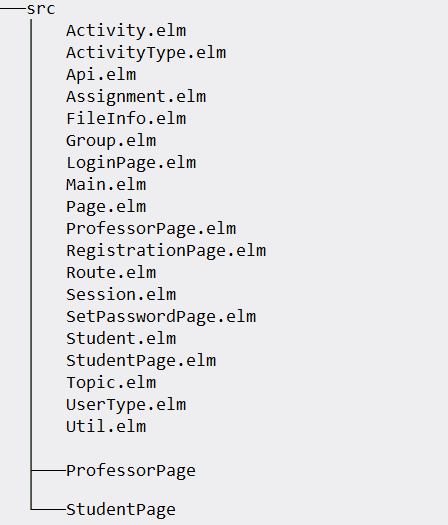
\includegraphics[width=0.5\textwidth]{msnr-elm-src.png}
  \caption{Organizacija \emph{Elm} datoteka unutar portala MSNR}
  \label{fig:msnr-elm-src}
\end{figure}

Aplikacija je podeljena na različite stranice koje se prikazuju u zavisnosti od trenutne \emph{url} putanje. 
U korenu projekta nalazi se osnovna datoteka \emph{Main.elm} u kojoj se nalazi funkcija \texttt{main} sa definicijom \emph{Elm} aplikacije.
Zajedno sa njom su i datoteke koje sadrže definicije osnovnih stranica, entiteta, putanja i modula za komunikaciju sa serverom, a
u posebnim direktorijumima odvojene su datoteke za prikazivanje studentskih i profesorskih stranica. U nastavku rada, zajedno sa načinom
rada \emph{Elm} aplikacije, biće prikazana uloga navedenih modula.

\section{Elm aplikacija}
U uvodnom delu rada, na primeru brojača, prikazan je najjednostavniji primer \emph{Elm} programa kreiran funkcijom \texttt{sandbox}.
Pored nje, u modulu \texttt{Browser} se nalaze funkcije \texttt{element}, \texttt{document} i \texttt{application}
kojima je implementiran korisnički interfejs portala MSNR.

Prethodno navedene četiri funkcije poređane su po kompleksnosti i svaka naredna pruža dodatne mogućnosti.
Funkcijom \texttt{element} se uvodi mogućnost komunikacije sa "spoljašnjim svetom" pomoću koncepta komande, supskripcije, portova
i oznaka (\emph{flags}). Pruža kontrolu nad jednim \emph{HTML} elementom i ova funkcija je veoma bitna za \emph{Elm} adaptaciju,
jer omogućava laku integraciju u postojeći \emph{JavaScript} projekat. 
Funkcija \texttt{document} proširuje funkciju \texttt{element} time što upravlja celim dokumentom i pruža kontrolu nad \emph{HTML} elementima \texttt{<title>}
i \texttt{<body>}. Na kraju, funkcija \texttt{application} kreira aplikaciju koja upravlja \emph{url} promenama, u primeru koda
\ref{listing:elm-application} prikazana je njena anotacija. 
\begin{listing}[h]
\begin{minted}[fontsize=\footnotesize]{haskell}
  application :
  { init : flags -> Url -> Key -> ( model, Cmd msg )
  , view : model -> Document msg
  , update : msg -> model -> ( model, Cmd msg )
  , subscriptions : model -> Sub msg
  , onUrlRequest : UrlRequest -> msg
  , onUrlChange : Url -> msg
  }
  -> Program flags model msg
\end{minted}
\caption{Tipovi funkcija}
\label{listing:elm-application}
\end{listing} 

Oznakama (\emph{flags}) je moguće prosleđivanje podataka \emph{Elm} programu iz \emph{JavaScript} koda.
Komande (\texttt{Cmd}) služe za izvršavanje akcija izvan okruženja \emph{Elm} (npr. \emph{HTTP} zahtevi), a supskripcijama
(\texttt{Sub}) je moguće pretplatiti se na određeni događaj. Polja \texttt{onUrlRequest} i \texttt{onUrlChange}, kao i
parametar \texttt{Url} funkcije \texttt{init}, koriste se za rad sa putanjama prilikom implementacije jednostranične aplikacije.
Navedeni koncepti i njihova upotreba unutar portala MSNR biće detaljnije objašnjeni dalje u radu.

\subsection{Inicijalizacija aplikacije}
Tip funkcije \texttt{init} prikazan je u primeru koda \ref{listing:elm-application} i kao argumente prihvata oznake, trenutnu putanju i ključ navigacije,
a povratna vrednost je torka modela i komande. Ključ navigacije generiše se prilikom inicijalizacije, obavezan je parametar prilikom menjanja
putanja unutar aplikacije i kao takav se mora čuvati u modelu. Pored ključa navigacije, u modelu se čuvaju informacije o trenutnom korisniku,
putanji i stranici koja se prikazuje. Takođe, model sadrži podatke o aktivnostima čiji sadržaj zavisi od trenutnog korisnika, adresu veb interfejsa,
dužinu trajanja tokena za pristup i oznaku da li je u toku inicijalno učitavanje aplikacije. Model aplikacije može se videti u primeru koda \ref{listing:elm-model},
a definisan je u datoteci \emph{Main.elm}.
\begin{listing}[h]
\begin{minted}[fontsize=\footnotesize]{haskell}
  type alias Model =
  { currentUser : UserType
  , currentRoute : Route
  , currentPage : Page
  , accessTokenExpiresIn : Float
  , key : Nav.Key
  , mainContent : ContentModel
  , initialLoading : Bool
  , apiBaseUrl : String
  }
\end{minted}
\caption{Definicija modela}
\label{listing:elm-model}
\end{listing}

Aplikacija je kompajlirana tako da se kreira datoteka \emph{app.js} koji se uključuje u dokument \emph{index.html},
čija je osnovna struktura prikazana u primeru koda \ref{listing:elm-index-html}. Pokreće se pozivanjem \texttt{init}
funkcije iz modula \texttt{Main} i tom prilikom se vrši prosleđivanje putanje ka veb interfejsu, tj. serverskom delu portala,
preko oznaka.
\begin{listing}[h]
\begin{minted}[fontsize=\footnotesize]{html}
<html>
  <head>
      <script src="/app.js"></script>
  </head>
  <body>
      <div id="app"></div>
      <script>
          var app = Elm.Main.init({
              node: document.getElementById("app"),
              flags: { apiBaseUrl : "http://localhost:4000/api" }
          });
      </script>
  </body>
</html>
\end{minted}
\caption{Pokretanje \emph{Elm} aplikacije}
\label{listing:elm-index-html}
\end{listing}
Prilikom inicijalizacije, trenutna stranica i putanja se određuju na osnovu \emph{url} vrednosti i
čuva se vrednost prosleđena oznakama. Takođe se proverava da li je trenutni korisnik autentifikovan
slanjem \emph{HTTP} zahteva za obnovu tokena. Korisnik je podrazumevano neautentifikovan dok se ne dobije
odgovor servera. 
\subsection{Komande}
Slanje \emph{HTTP} zahteva, generisanje slučajnih brojeva, određivanje trenutnog vremena i slične operacije
mogu imati različite rezultate ukoliko se izvrše više puta. Kao takve, ne mogu se predstaviti \emph{Elm}
funkcijama već se za to koriste komande.

Komanda predstavlja vrednost koja opisuje operaciju koju okruženje \emph{Elm} treba da izvrši.
Rezultat izvršene operacije se preko poruke prosleđuje funkciji \texttt{update}. Tako da se svako
izvršavanje komandi posmatra kao ulazni podatak aplikacije čime se garantuje da sve funkcije budu
čiste, iako se izvršavaju operacije koje to nisu.

Definicija komande --- \texttt{type \textbf{Cmd} msg} nalazi se unutar modula \emph{Platform.Cmd} 
u osnovnom paketu \emph{elm/core}, gde \texttt{msg} predstavlja tip poruke koja se vraća aplikaciji.
Funkcija \texttt{Cmd.none} se koristi kada nema komandi za izvršavanje, a ukoliko je potrebno izvršiti
više operacija koristi se \texttt{Cmd.batch}.

Inicijalna komanda se izvršava samo prilikom pokretanja aplikacije, centralno mesto izvršavanja komandi
predstavlja funkcija \texttt{update}, čiji je povratni tip, kao i kod funkcije \texttt{init}, proširen sa \texttt{\textbf{Cmd} msg}.
Ilustracija funkcije \texttt{update} sa komandama unutar arhitekture \emph{Elm} prikazan je na slici \ref{fig:elm-command}.
\begin{figure}[!h]
  \centering
  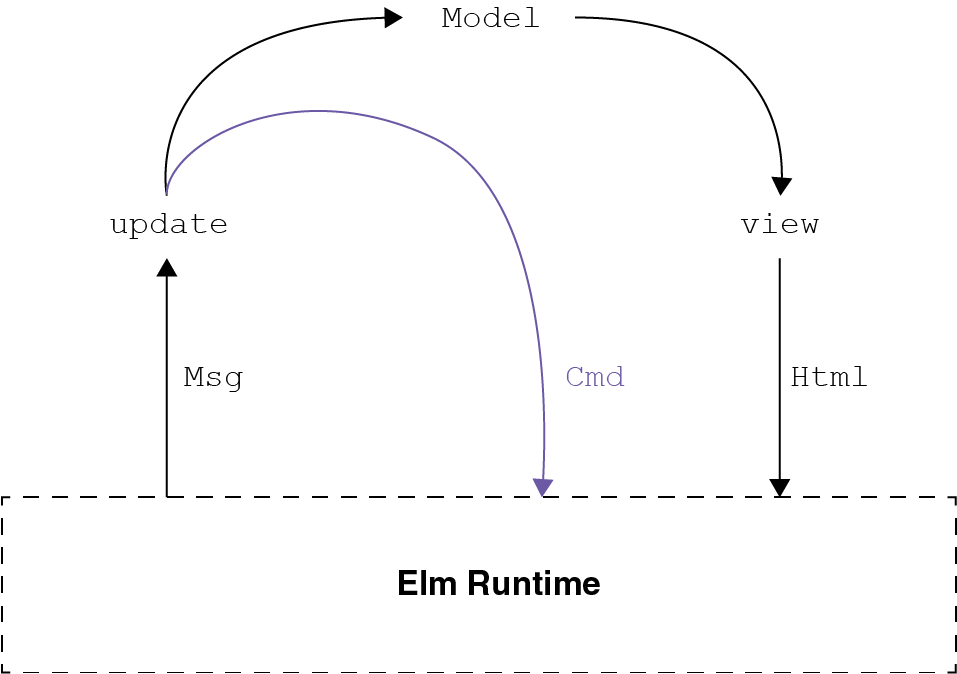
\includegraphics[width=0.6\textwidth]{elm-command.png}
  \caption{Tok komandi unutar arhitekture \emph{Elm}}
  \label{fig:elm-command}
\end{figure}

\subsection{Komunikacija sa serverom}
Kreiranje komandi za slanje \emph{HTTP} zahteva izvršava se pomoću paketa \emph{elm/http}.
Osnovna funkcija unutar paketa je \texttt{request}, čija je anotacija prikazana u primeru koda \ref{listing:elm-request}.
\begin{listing}[h]
\begin{minted}[fontsize=\footnotesize]{haskell}
  request :
  { method : String
  , headers : List Header
  , url : String
  , body : Body
  , expect : Expect msg
  , timeout : Maybe Float
  , tracker : Maybe String
  }
  -> Cmd msg
\end{minted}
\caption{Anotacija funkcije \texttt{Http.request}}
\label{listing:elm-request}
\end{listing}

Polja \texttt{method}, \texttt{headers}, \texttt{url}, \texttt{body} i \texttt{timeout} označavaju standardna
svojstva \emph{HTTP} zahteva. Poljem \texttt{expect} se označava koji tip podataka se očekuje kao odgovor i kojom porukom
će se ažurirati aplikacija. Polje \texttt{tracker} služi za praćenje progresa zahteva, ali kao ni \texttt{timeout},
nije korišćeno u aplikaciji. Pored funkcije \texttt{request} i funkcija \texttt{riskyRequest} koja ima istu anotaciju, s tim što omogućava
postavljanje kolačića od strane servera (uključuje opciju \texttt{withCredentials} \cite{withCredentials}).

Za komuniciranje sa veb interfejsom portala MSNR kreiran je modul \emph{Api} koji otkriva funkcije \texttt{get}, \texttt{post},
\texttt{put} i \texttt{delete} koje se oslanjaju na \texttt{request}, kao i funkcije koje se oslanjaju na
\texttt{riskyRequest} --- \texttt{getWithCredentials} i \texttt{postWithCredentials}. Takođe, unutar modula
su navedene sve putanje veb interfejsa koje se korste u aplikaciji.
Anotacija funkcije \texttt{get} prikazana je u primeru koda \ref{listing:elm-api-get}. 
\begin{listing}[h]
  \begin{minted}[fontsize=\footnotesize]{haskell}
    get :
    { apiBaseUrl : String
    , endpoint : String
    , token : String
    , expect : Http.Expect msg
    }
    -> Cmd msg
  \end{minted}
  \caption{Anotacija funkcije \texttt{Api.get}}
  \label{listing:elm-api-get}
  \end{listing}
Prilikom slanja zahteva MSNR veb interfejsu potrebno je proslediti token za autorizaciju,
osnovnu adresu i krajnju tačku (nastavak putanje) kojom se određuje resurs kom se pristupa.
U slučaju \texttt{post} i \texttt{put}, dodaje se i telo zahteva pored prikazanih parametara.

Funkcije \texttt{getWithCredentials} i \texttt{postWithCredentials} koriste se za obnavljanje tokena,
prijavljivanje i odjavljivanje korisnika i njihova upotreba izdvojena je u poseban modul \emph{Session}.
Deo modula \emph{Session} sa definicijom poruka i funkcije za obnavljanje tokena
prikazan je u primeru koda \ref{listing:elm-session}.
\begin{listing}[h]
\begin{minted}[fontsize=\footnotesize]{haskell}
  type alias Session =
    { accessToken : String
    , expiresIn : Float
    , userInfo : UserInfo
    , semesterId : Int
    , studentInfo : Maybe StudentInfo
    }

  type Msg
    = GotSessionResult (Result Http.Error Session)
    | GotTokenResult (Result Http.Error Session)
    | DeleteSessionResult (Result Http.Error ())

  silentTokenRefresh : String -> Cmd Msg
  silentTokenRefresh apiBaseUrl =
      Api.getWithCredentials
          { apiBaseUrl = apiBaseUrl
          , endpoint = Api.endpoints.refreshToken
          , expect = Http.expectJson GotTokenResult decodeSession
          }
\end{minted}
\caption{Definicija funkcije \texttt{silentTokenRefresh}}
\label{listing:elm-session}
\end{listing}
Ukoliko u kolačiću postoji validan token za obnavljanje, server će vratiti \emph{JSON} objekat koji sadži token za pristupanje i informacije o trenutnom korisniku.
Očekivani rezultat odgovara slogu \texttt{Session}. Funkcija \texttt{Http.expectJson} prima dva argumenta --- poruka kojom se rezultat komande prosleđuje aplikaciji
i dekoder kojim se \emph{JSON} objekat mapira u slog \texttt{Session}. 

Rad sa \emph{JSON} podacima (kodiranje i dekodiranje) izvršava se pomoću modula \emph{Json.Encode} i \emph{Json.Decode} iz paketa \emph{elm/json}.
Funkcija \texttt{decodeSession} iz prethodnog primera sa upotrebom funkcija za dekodiranje prikazana je u primeru koda \ref{listing:elm-decoder}.
\begin{listing}[h]
\begin{minted}[fontsize=\footnotesize]{haskell}
  decodeSession : Decoder Session
  decodeSession =
      Decode.map5 Session
          (Decode.field "access_token" Decode.string)
          (Decode.field "expires_in" Decode.float)
          (Decode.field "user" decodeUser)
          (Decode.field "semester_id" Decode.int)
          (Decode.maybe (Decode.field "student_info" decodeStudentInfo))
\end{minted}
\caption{Definicija funkcije \texttt{silentTokenRefresh}}
\label{listing:elm-decoder}
\end{listing}
Unutar dekodera mogu se pozivati i drugi dekoderi što se može videti na primeru \texttt{decodeUser} i \texttt{decodeStudentInfo}.
Ovakva obrada \emph{JSON} podataka pruža validaciju podataka pre nego što oni dođu do aplikacije. Ukoliko podaci nemaju očekivanu strukturu
definisanu u dekoderu dobija se greška \texttt{BadBody}.

\subsection{Supskripcije}
Nakon inicijalizacije, obnavljanje tokena se izvršava svaki put kada istekne period važenja tokena za pristup.
Budući da se tada komande mogu izvršavati samo unutar funkcije \texttt{update}, potrebno je nekako proslediti poruku
kojom će se komanda obnavljanja izazvati. To upravo omogućavaju supskripcije.

Supskripcije predstavljaju način da se određeni događaji izvan \emph{Elm} programa prevedu u
poruku koja će biti prosleđena funkciji \texttt{update}. Kao i komande, definisane su unutar paketa \emph{elm/core}
i mogu se koristiti funkcije \texttt{Sub.none} i \texttt{Sub.batch}.
U primeru koda \ref{listing:elm-subscriptions} prikazana je supskripcija za obnavljanje
tokena. Funkcijom \texttt{Time.every} se periodično, na određeni broj milisekundi uzima trenutno vreme i prosleđuje se
aplikaciji preko poruke. 
\begin{listing}[h]
\begin{minted}[fontsize=\footnotesize]{haskell}
subscriptions : Model -> Sub Msg
subscriptions { currentUser, accessTokenExpiresIn } =
    let
        refreshTick =
            case currentUser of
                Guest ->
                    Sub.none

                _ ->
                    Time.every (1000 * (accessTokenExpiresIn - 5)) RefreshTick
    in
    Sub.batch [ refreshTick ]
\end{minted}
\caption{Supskripcija za obnavljanje tokena}
\label{listing:elm-subscriptions}
\end{listing}

\section{Moduli stranica i putanja aplikacije}
Definicija svih putanja aplikacije nalazi se u modulu \emph{Route} i prikazane su u primeru koda \ref{listing:elm-routes}.
Profesorskih putanja ima više i definisane su posebnim tipom, takođe unutar istog modula.
\begin{listing}[h]
\begin{minted}[fontsize=\footnotesize]{haskell}
  type Route
    = Home
    | Student
    | Login
    | Registration
    | Professor ProfessorSubRoute
    | SetPassword String
    | NotFound
\end{minted}
\caption{Putanje aplikacije}
\label{listing:elm-routes}
\end{listing}
Prilikom inicijalizacije aplikacije, upotrebom funkcije \texttt{Route.fromUrl} vrši se parsiranje trenutne
\emph{url} putanje iz pregledača i mapira se na jednu od definisanih putanja. Sve nevalidne putanje 
predstavljaju se putanjom \texttt{NotFound}. U slučaju putanje \texttt{SetPassword} očekuje se univerzalni
identifikator za postavljanje lozinke kao deo putanje.

Modul \emph{Route} sadrži funkciju \texttt{guard} za sprečavanje
neautorizovanog pristupa određenim stranicama i funkciju \texttt{redirectTo} za kreiranje
komande promene putanje. Funkcija \texttt{redirectTo} poziva funkciju \texttt{pushUrl} iz modula
\emph{Browser.Navigation} koja koristi navigacioni ključ. Nakon izvršavanja komande,
nova putanja se prosleđuje funkciji \texttt{update} kroz poruku navedenu kao \texttt{onUrlChange} prilikom
pokretanja aplikacije. Poruka navedena u drugom polju --- \texttt{onUrlRequest} emituje se prilikom klika na
vezu unutar aplikacije. 

Osnovna podela aplikacije jeste na stranice koje se koriste za prijavljivanje i registraciju korisnika
(moduli \emph{LoginPage}, \emph{RegistrationPage} i \emph{SetPasswordPage}), studentsku stranicu (modul \emph{StudentPage})
i profesorske stranice kojima se koordiniše kroz modul \emph{ProfessorPage}. Pored njih, tu su i stranice koje nisu izdvojene u
posebne module --- početna i stranica koja se prikazuje u slučaju pogrešne putanje. Definicija tipova stranica prikazanih u
primeru koda \ref{listing:elm-pages} nalazi se u modulu \emph{Page}, a definicija profesorskih podstranica se nalazi u modulu \emph{ProfessorPage}.
\begin{listing}[h]
\begin{minted}[fontsize=\footnotesize]{haskell}
  type Page
    = HomePage
    | LoginPage LP.Model
    | RegistrationPage RP.Model
    | SetPasswordPage SPP.Model
    | ProfessorPage
    | StudentPage
    | NotFoundPage
\end{minted}
\caption{Stranice aplikacije}
\label{listing:elm-pages}
\end{listing}
Stanje, odnosno model, studentskih i profesorskih stranica čuva se u glavnom modelu pod poljem \texttt{mainContent}.
Stranice koje se koriste za prijavljivanje i registrovanje korisnika uključuju svoje modele u tip
i unutar glavnog modela se nalaze pod poljem \texttt{currentPage}. Unutar modula \emph{Page}
nalazi se funkcija \texttt{forRoute} kojim se na osnovu date putanje kreira odgovarajuća stranica.

Svaka stranica koja ima svoj modul ima i definisan svoj model, poruke, kao i funkcije \texttt{update} i \texttt{view} koje
se pozivaju iz glavnog modula aplikacije. Poruke svih stranica, zajedno sa ostalim porukama aplikacije, objedinjuju
se unutar modula \emph{Main} u glavni tip poruke (primer koda \ref{listing:elm-msgs}).
\begin{listing}[h]
  \begin{minted}[fontsize=\footnotesize]{haskell}
    type Msg
      = ClickedLink Browser.UrlRequest
      | ChangedUrl Url
      | GotProfessorMsg ProfessorPage.Msg
      | GotStudentMsg StudentPage.Msg
      | GotLoginMsg Login.Msg
      | GotRegistrationMsg Registration.Msg
      | GotPasswordMsg SetPassword.Msg
      | GotInitSessionMsg Session.Msg
      | GotSessionMsg Session.Msg
      | RefreshTick Time.Posix
      | Logout
  \end{minted}
  \caption{Objedinjene poruke aplikacije}
  \label{listing:elm-msgs}
  \end{listing}
Unutar funkcijie \texttt{update} glavnog modula se na osnovu poruke poziva funkcija \texttt{update}
odgovarajuće stranice. Trenutni model se ažurira novim modelom date stranice, a poruku rezultujuće komande je potrebno
transformisati u odgovarajući glavni tip poruke. Primer ažuriranja studentske stranice dat je u primeru koda \ref{listing:elm-update}.
Analogno ažuriranju, unutar glavne funkcije \texttt{view} se na osnovu trenutne stranice poziva funkcija \texttt{view} odgovarajućeg modula.  
\begin{listing}[h]
\begin{minted}[fontsize=\footnotesize]{haskell}
  update msg model =
      case ( msg, model.currentPage, model.mainContent ) of
          ...
          ( GotStudentMsg studentMsg, _, StudentModel model_ ) ->
          let
              ( studentModel, cmd ) =
                  StudentPage.update studentMsg model_
          in
          ( { model | mainContent = StudentModel studentModel }
          , cmd |> Cmd.map GotStudentMsg
          )
          ...
\end{minted}
\caption{Ažuriranje studentske stranice}
\label{listing:elm-update}
\end{listing} 


\section{Stilizovanje aplikacije}
\emph{Elm} kao jezik specijalne namene sadrži sve što je potrebno za razvoj korisničkog interfejsa veb aplikacija.
Zgodno je, ipak, iskoristiti gotove, stilizovane komponente (npr. modale, tabove i slično) kako ne bismo
implementirali sve od početka.

Za potrebe implementacije portala MSNR korišćen je paket \emph{NoRedInk/noredink-ui},
koji se oslanja na dosta drugih paketa među kojima je bitno izdvojiti paket 
\emph{tesk9/accessible-html-with-css}.
Ovaj paket predstavlja proširenje paketa \emph{rtfeldman/\\elm-css} koji se takođe koristi u projektu
i omogućava stilizovanje \emph{HTML} elemenata unutar programskog jezika \emph{Elm}, bez upotrebe
\emph{css} datoteka. Za iscrtavanje \emph{HTML} elemenata koriste se odgovarajuće funkcije iz
modula \emph{Html.Styled} umesto iz modula \emph{Html}.

\begin{listing}[h]
\begin{minted}[fontsize=\footnotesize]{haskell}
import Accessibility.Styled as Html exposing (Html)
import Browser exposing (Document)
import Css exposing (..)
import Html.Styled.Attributes exposing (css, href)
...
view_ : Model -> Html Msg
view_ model =
    ... 
    Html.div
        [ css [ height (vh 100), displayFlex, flexDirection column ] ]
        [ {-sadrzaj-}
        ]

view : Model -> Document Msg
view model =
    { title = "MSNR"
    , body = [ view_ model |> Html.toUnstyled ]
    }
\end{minted}
\caption{Primer stilizovanja elementa i upotreba funkcije \texttt{toUnstyled}}
\label{listing:elm-toUnstyled}
\end{listing}

Modul \emph{Accessibility.Styled} iz paketa \emph{tesk9/accessible-html-with-css} pored stilizovanja pruža i podršku za pristupačnost \cite{a11y}
(eng. \emph{accessibility} --- skraćeno \emph{a11y}). Funkcija \texttt{toUnstyled} omogućava korišćenje \emph{Accessibility.Styled.Html} unutar \emph{Elm} aplikacije.
Primer njene upotrebe unutar modula \emph{Main} prikazan je u primeru koda \ref{listing:elm-toUnstyled}.

\section{Struktura profesorske stranice}
Profesorske stranice nalaze se pod direktorijumom \emph{ProfessorPage} (slika \ref{fig:prof-dir}).
Svaka stranica predstavljena je zasebnim modulom i to su:
\begin{itemize}
  \item \emph{RegistrationRequestsPage} --- za obradu studentskih zahteva za registraciju,
  \item \emph{ActivitiesPage} --- za dodavanje novih aktivnosti,
  \item \emph{GroupsPage} --- za prikazivanje svih grupa,
  \item \emph{TopicsPage} --- za dodavanje tema studentskih radova,
  \item \emph{ActivityAssignmentPage} --- za pregled i ocenjivanje studentskih aktivnosti.
\end{itemize}

\begin{figure}[!ht]
  \centering
  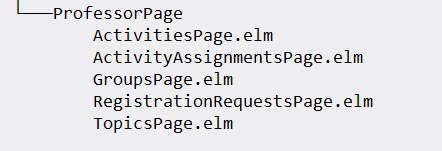
\includegraphics[width=0.5\textwidth]{prof-page-dir.png}
  \caption{Sadržaj direktorijuma \emph{ProfessorPage}}
  \label{fig:prof-dir}
\end{figure}

Prikazivanje odgovarajućih stranica u odnosu na trenutnu putanju obrađuje se unutar modula
\emph{ProfessorPage}, slično obradi svih stranica unutar modula \emph{Main}. 
Svaka stranica ima svoj model, kao i funkcije \texttt{view} i \texttt{update}.
Model definisan u modulu \emph{ProfessorPage} sadrži sve modele stranica
kao i zajedničke podatke o studentima, grupama i aktivnostima. 
\begin{listing}[h]
\begin{minted}[fontsize=\footnotesize]{haskell}
type alias Model =
  { zone : Zone
  , accessToken : Token
  , apiBaseUrl : String
  , currentSemesterId : Int
  , requstesModel : Requests.Model
  , activitiesModel : Activities.Model
  , activityAssignmentsModel : ActivityAssignments.Model
  , topicsModel : TopicsPage.Model
  , activities : Dict Int Activity
  , activityTypes : Dict Int ActivityType
  , groups : Dict Int Group
  , students : Dict Int Student
  , assignments : List ShallowAssignment
  , loadingActivities : Bool
  , loadingActivityTypes : Bool
  , loadingGroups : Bool
  , loadingStudents : Bool
  , loadingAssignment : Bool
  , hasLoadingError : Bool
  }
\end{minted}
\caption{Glavni model za prikazivanje profesorskih stranica}
\label{listing:prof-model}
\end{listing}
U primeru koda \ref{listing:prof-model} prikazan je alijas sveobuhvatnog modela, gde se pored
modela stranica mogu videti i ostali podaci potrebni za njihovo prikazivanje.
Modeli stranica čuvaju podatke koji se koriste isključivo unutar odgovarajuće stranice.
Prilikom prikazivanja profesorskih stranica u modulu \emph{ProfessorPage}
poziva se funkcija \texttt{view} odgovarajuće stranice, kojoj se prosleđuje adekvatan
model, zajedno sa drugim potrebnim podacima.

Kretanje kroz stranice vrši se pomoću navigacione trake čiji prikaz se može videti na
slici \ref{fig:professor-page} zajedno sa izgledom stranice za ocenjivanje aktivnosti.
\begin{figure}[!ht]
  \centering
  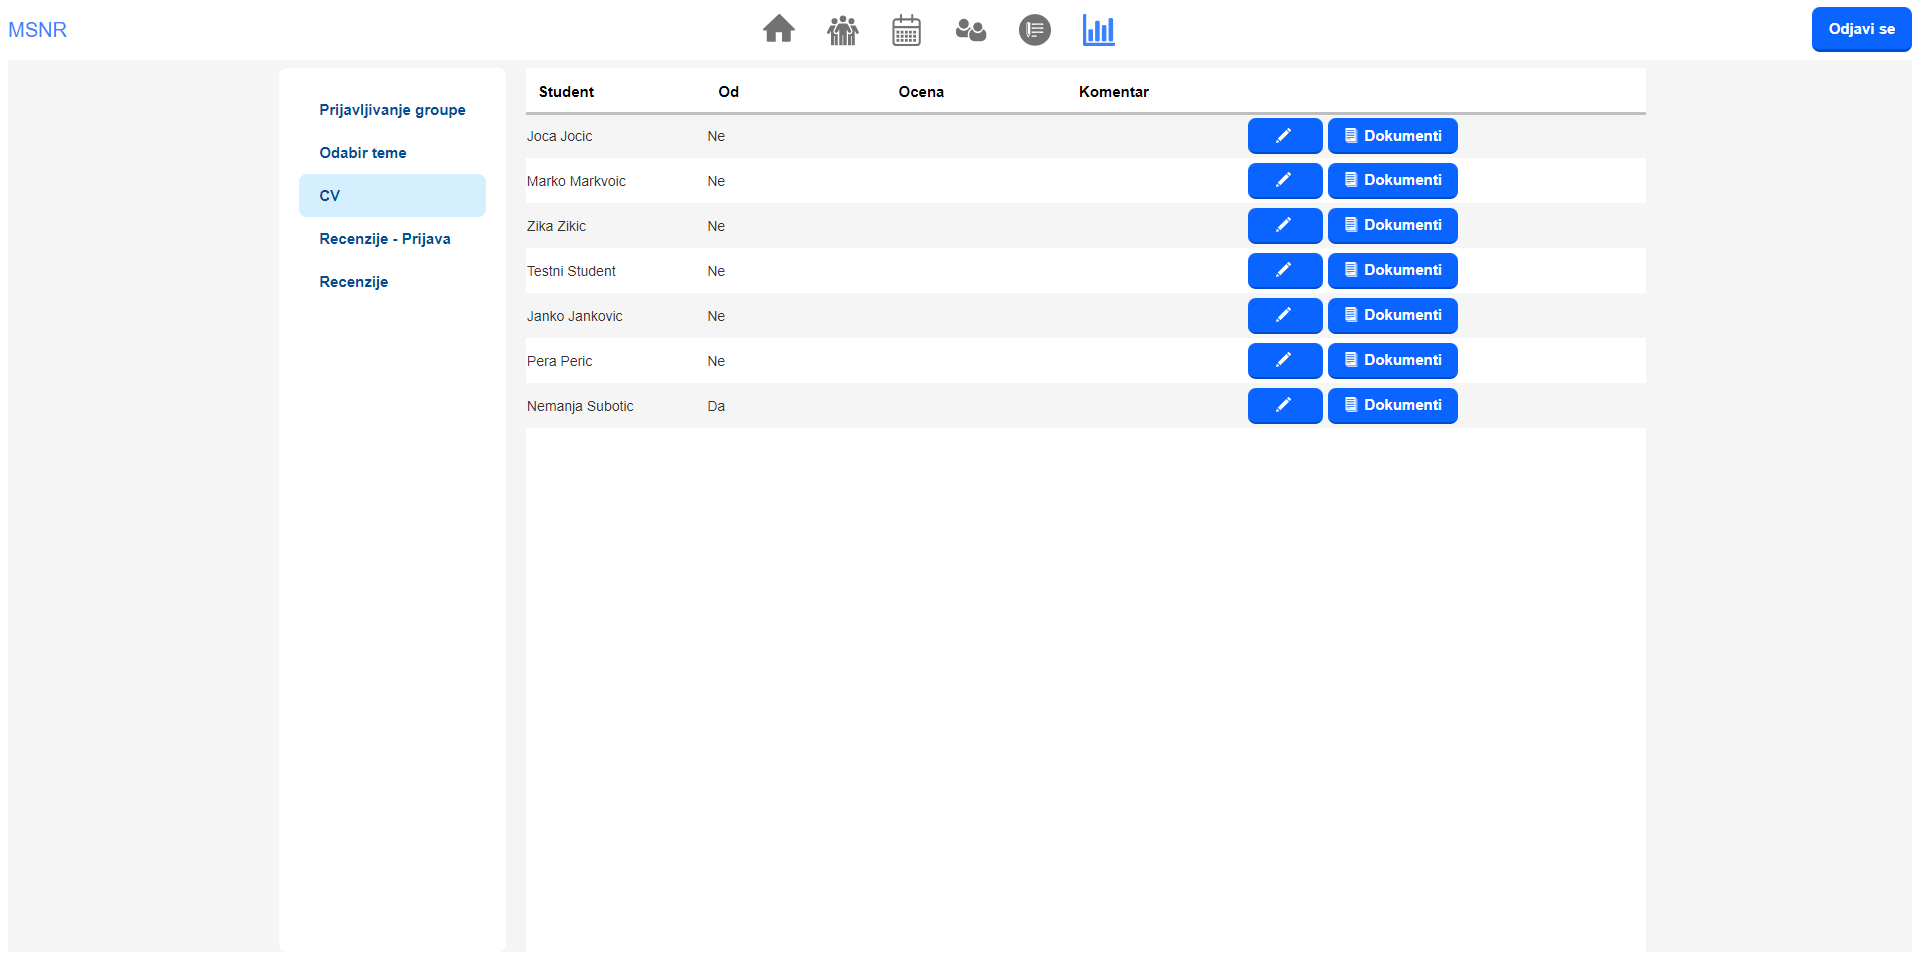
\includegraphics[width=0.9\textwidth]{professor-page.png}
  \caption{Izgled stranice za ocenjivanje aktivnosti}
  \label{fig:professor-page}
\end{figure}
\section{Struktura studentske stranice}
Za razliku od profesorskog dela aplikacije koji je podeljen na više stranica,
studentski deo se sastoji iz samo jedne stranice u kojoj su prikazane sve dodeljene
aktivnosti studenta. 

Svaka dodeljena aktivnost ima naziv i opis aktivnosti, rok za izvršenje
i broj poena koji nosi. Način prikazivanja pojedinačnih aktivnosti razlikuje se po
jedinstvenom kodu i sadržaju tipa aktivnosti, kao i po tome da li je u pitanju prijava
za aktivnost. Tako da se prikazivanje same aktivnosti može podeliti u dva dela,
jedan se odnosi na osnovne podatke, a drugi na sam sadržaj aktivnosti potreban za prijavljivanje grupe,
tema, prilaganja dokumenata ili prijavljivanje za određenu aktivnost.

Prikazivanje studentske stranice obrađuje se unutar modula \emph{StudentPage},
a pomoćni moduli koji se tom prilikom koriste nalaze se pod direktorijumom \emph{StudentPage} čija je
struktura prikazana na slici \ref{fig:student-dir}.
\begin{figure}[!ht]
  \centering
  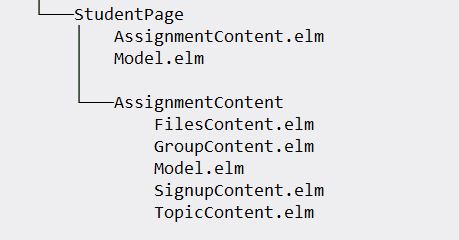
\includegraphics[width=0.5\textwidth]{student-dir.png}
  \caption{Sadržaj direktorijuma \emph{StudentPage}}
  \label{fig:student-dir}
\end{figure}

Modeli studentske stranice i sadržaja aktivnosti izdvojeni su u posebne module --- \emph{StudentPage.Model} i
\emph{AssignmentContent.Model} da bi se izbegla ciklična zavisnost, jer se osnovni model koristi unutar
modula \emph{AssignmentContent}. U primeru koda \ref{listing:student-model} predstavljen je osnovi model studentske stranice u kom se
nalaze svi podaci potrebni za njen prikaz.
\begin{listing}[h]
\begin{minted}[fontsize=\footnotesize]{haskell}
    type alias Model =
      { accessToken : Token
      , apiBaseUrl : String
      , email : String
      , firstName : String
      , lastName : String
      , studentId : Int
      , semesterId : Int
      , groupId : Maybe Int
      , loadingGroup : Bool
      , group : Maybe Group
      , indexNumber : String
      , zone : Zone
      , currentTimeSec : Int
      , loading : Bool
      , assignments : Array Assignment
      , assignmentsModels : Array ACM.Model
      , assignmentsState : AssignmentsState
      , loadingStudents : Bool
      , students : List Student
      , loadingTopics : Bool
      , topics : List Topic
      }
\end{minted}
\caption{Osnovni model za prikazivanje studentske stranice}
\label{listing:student-model}
\end{listing}
Za razliku od modela profesorskih stranica, modeli sadržaja aktivnosti čuvaju se u nizu
(\texttt{assignmentsModels}). Svakom elementu niza modela odgovara dodeljena aktivnost (niz \texttt{assignments}) na istom indeksu.

Osnovni modul za prikazivanje studentske stranice, pored modula \emph{StudentPage}, jeste modul
\emph{AssignmentContent} koji ima sličnu ulogu kao modul \emph{ProfessorPage} kod profesorskih
stranica. U direktorijumu \emph{AssignmentContent} nalaze se moduli za obradu sadržaja --- \emph{GroupContent}, \emph{FilesContent},
\emph{SignupContent} i \emph{TopicContent}, i kao kod profesorskih stranica svaki od njih ima svoj
model i funkcije \texttt{update} i \texttt{view}.

Prilikom pozivanja funkcije \texttt{update} u modulu \emph{StudentPage} unutar poruke (\texttt{Msg}), pored informacije o
samoj poruci, nalazi se i indeks na osnovu kog se menja odgovarajući model u nizu. Definisanje poruke sa indeksom i njena
obrada prikazana je u primeru koda \ref{listing:student-update}.
\begin{listing}[h]
\begin{minted}[fontsize=\footnotesize]{haskell}
  type Msg
    = ...
    | GotAssignmentContentMsg Int AssignmentContent.Msg

  update : Msg -> Model -> ( Model, Cmd Msg )
  update msg model =
  ...
  GotAssignmentContentMsg index assignmentMsg ->
  let
      ( model_, cmd ) =
          AssignmentContent.update assignmentMsg index model
  in
  ( model_, Cmd.map (GotAssignmentContentMsg index) cmd )
\end{minted}
\caption{Ažuriranje sadržaja aktivnosti}
\label{listing:student-update}
\end{listing}
Funkcija \emph{AssignmentContent} iz modula \emph{AssignmentContent} na osnovu tipa poruke poziva
funkciju ažuriranja iz odgovarajućeg modela za obradu sadržaja.

Za prikazivanje dodeljenih aktivnosti koristi sa komponenta harmonika (eng. \emph{accordion}) iz paketa \emph{NoRedInk/noredink-ui},
tako da se inicijalno prikazuju samo zaglavlja aktivnosti sa osnovnim informacijama.
\begin{figure}[!ht]
  \centering
  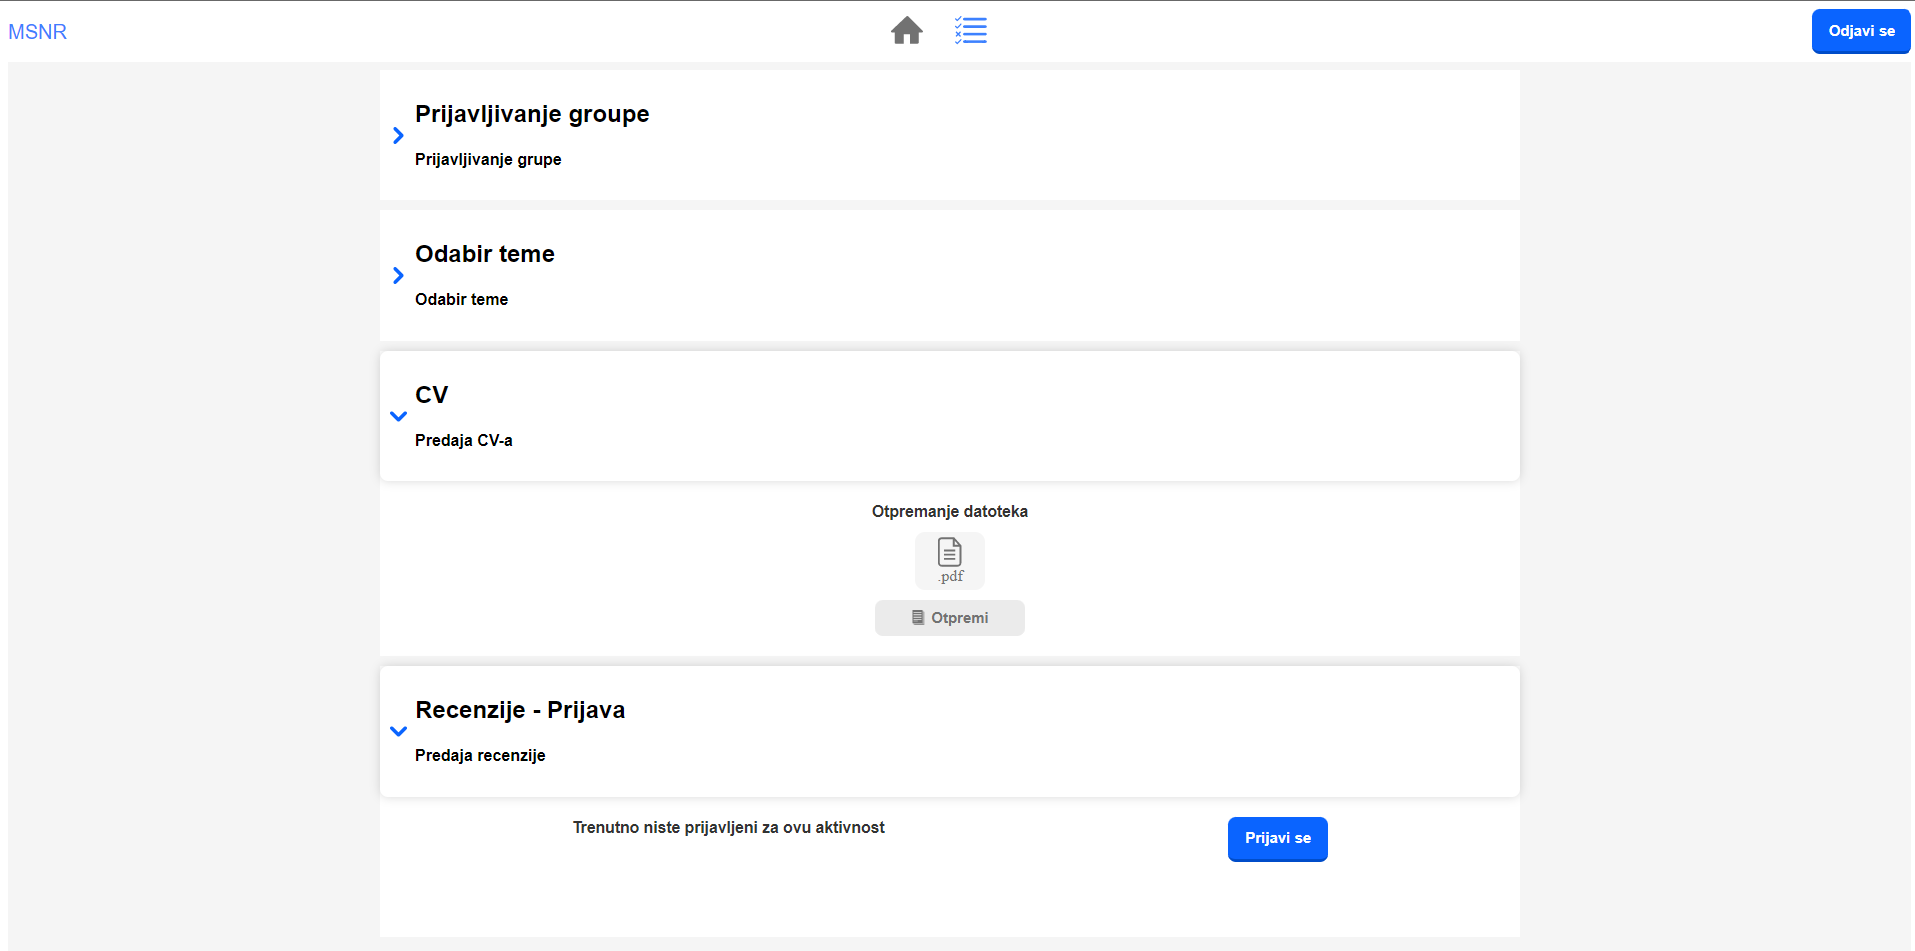
\includegraphics[width=0.9\textwidth]{student-page.png}
  \caption{Izgled studentske stranice}
  \label{fig:student-page}
\end{figure}
Klikom na zaglavlje prikazuje se i sam sadžaj aktivnosti. Izgled studentske stranice prikazan je na slici \ref{fig:student-page}.
Prikazivanje zaglavlja aktivnosti definiše se unutar modula \emph{StudentPage}, a za prikazivanje sadržaja, analogno ažuriranju,
poziva se funkcija \emph{view} iz modula \emph{AssignmentContent}.

% ------------------------------------------------------------------------------
\chapter{Zaključak}
% ------------------------------------------------------------------------------
U ovom radu predstavljen je razvoj studentskog portala upotrebom funkcionalinih
programskih jezika \emph{Elm} i \emph{Elixir}. Sam portal predstavlja prototip na
kom su prikazane osnovne osobine i koncepti ovih programskih jezika. U okviru rada
data su objašnjenja osnovnih funkcionalnosti i komponenti portala, kao i
objašnjenje implementacije najvažnijih delova.

Razvojni okvir \emph{Phoenix} daje jasne smernice kako struktura projekta treba
da izgleda. Biblioteke unutar ekosistema \emph{Elixir} nastale su na osnovu dobrih
praksi postojećih biblioteka drugih programskih jezika što njihovu adaptaciju
čini lakom. Stoga, rad sa razvojnim okvirom \emph{Phoenix} deluje poznato, a
posebnu udobnost u radu, u odnosu na druga razvojna okruženja, pružaju izraženo poklapanje
obrazaca i njegova funkcionalna priroda. Iako se za osnovnu prednost \emph{Phoenix}-a
uzima izvršavanje na virtualnoj mašini \emph{BEAM}, autor definitivno preporučuje njegovu
upotrebu za razvoj svih tipova veb aplikacija.

Sa druge strane, rad sa programskim jezikom \emph{Elm}, sa njemu svojstvenom arhitekturom
\emph{Elm} kao centralnim delom, predstavlja potpuno novo iskustvo.
Nakon početnog prilagođavanja na sam jezik i način
izvršavanja programa, rad sa programskim jezikom \emph{Elm} postaje vrlo
ugodan i daje poseban osećaj sigurnosti tokom rada u odnosu na programski jezik
\emph{JavaScript} (i razvojnim okvirima zasnovanim na njemu). Kompilator proverom tipova
garantuje ispravnost ulaznih podataka i forsira proveru svih slučajeva upotrebom tipova
\texttt{Maybe} i \texttt{Result}, što značajno smanjuje broj grešaka u aplikaciji.
Prilikom razvoja portala, korisnički interfejs je prošao
kroz nekoliko iteracija i značajnih izmena tokom kojih se sam autor uverio u lakoću
refaktorisanja koju \emph{Elm} zajedno sa kompilatorom pruža programerima.
U toku rada nije predsavljena integracija sa \emph{JavaScript}-om, koja je moguća, ali
podrazumeva uvođenje dosta šablonskog koda. Stoga, \emph{Elm} ne predstavlja pravi izbor
za razvoj aplikacija koje se zasnivaju na velikom broju biblioteka napisanjih u programskom
jeziku \emph{JavaScript}.

Pre upotrebe portala trebalo bi ubaciti podršku za telemetriju na serverskoj strani
u cilju nadgledanja rada aplikacije. 
Sadržaj tipa aktivnosti trenutno podržava samo rad sa dokumentima, dodavanjem podrške za
kreiranje prilagođenih formi zaokružile bi se sve aktivnosti unutar portala i pružila
mogućnost sprovođenja anketa i sličnih aktivnosti.
Kao značajnije unapređenje portala trebalo bi razmotriti
upotrebu rešenja za čuvanje dokumenata na oblaku. Na klijentskoj strani potrebno je
prilagoditi upotrebu korisničkog interfejsa za manje uređaje kao što su mobilni telefoni i tableti.

% ------------------------------------------------------------------------------
% Literatura
% ------------------------------------------------------------------------------
\literatura


% ==============================================================================
% Završni deo teze i prilozi
\backmatter
% ==============================================================================

% ------------------------------------------------------------------------------
% Biografija kandidata
\begin{biografija}
Nemanja Subotić rođen je 04.09.1993. godine u Užicu, odrastao je u Novoj Varoši,
gde je završio prirodno-matematički smer gimnazije "Pivo Karamatijević".
Smer \emph{Informatika} na Matematičkom fakultetu Univerziteta u Beogradu upisuje
2012. godine u septembru i završava u julu 2015. sa prosečnom ocenom \emph{9,38}.
Iste godine upisuje i master studije.

Od marta 2016. godine radi kao softverski inženjer na različitim projektima u
nekiliko domaćih i stanih firmi. Veći deo karijere radio je na razvoju veb
aplikacija odakle je i potekla ideja za temu rada.
\end{biografija}
% ------------------------------------------------------------------------------

\end{document}